\documentclass[11pt,oneside,openany]{memoir}
\input{/Users/gcrescenzo/Documents/School/LaTeX Documents/latex-class-notes/preamble-notes.tex}
\input{/Users/gcrescenzo/Documents/School/LaTeX Documents/latex-class-notes/makros.tex}
\renewcommand*{\mathbf}[1]{\varmathbb{#1}}
\renewcommand*{\emph}[1]{\textit{#1}}

\renewcommand{\projecttitle}{Thesis}




\begin{document}
%This adds a "front cover" page.
%{\thispagestyle{empty}
%\vspace*{\fill}
%\begin{tabular}{l}
%\begin{tabular}{l}
%\includegraphics[scale=0.24]{oxy-logo.png}
%\end{tabular} \\
%\begin{tabular}{l}
%\Large \color{black} Module Theory, Linear Algebra, and Homological Algebra \\ \Large \color{black} Gianluca Crescenzo
%\end{tabular}
%\end{tabular}
%\newpage
    \pagenumbering{roman}
    \chapter*{Preface}
    At the root of measure theory is a rigorous treatment of how to extend the notions of length (on the real line), area (on the Euclidean plane), and volume (in three-space) to a larger collection of sets than those seen in, say, courses on Calculus. We have seen in a first course in analysis that there exist sets with some exceptionally strange properties (the Cantor set being a classic example). We would like to be able to discuss these types of sets in the context of measuring their sizes (be it a length, area, volume, etc). While the historical impetus was to solve this problem for sets in $\bfR^n$, one finds that it is not hard to abstract the theory to more general sets. Accordingly we take up this abstract study. This is not just for the sake of abstraction. In fact one can find applications for abstract measure theory in, for example, probability theory (where the measure of a set corresponds to the likelihood of an element in that set being chosen under some random process) and physics (where one might want the measure of a set to correspond to the mass of some object occupying that space). 
    \vspace{-25pt}
    \tableofcontents
    \vfill
    \specialdate
    Last update: \today

    %\chapter{Preliminaries}
\pagenumbering{arabic}
\section{Set Theory}

    \begin{definition}
        A \textit{set} is a collection of different things; the things are called \textit{elements} of the set.
    \end{definition}

    Zermelo–Fraenkel set theory introduces eight different axioms which mathematics builds upon. Below is an introduction to the ones which are relevant for the material covered in this course.

    \begin{axiom}[Axiom of Extension]
        If the sets $X$ and $Y$ have the same members, then they are the same set. In other words:
            \begin{equation*}
            \begin{split}
                (\forall X)(\forall Y)\Bigl((\forall z)\bigl(z \in X \Leftrightarrow z \in Y\bigr) \implies X = Y\Bigr)
            \end{split}
            \end{equation*}
    \end{axiom}

    \begin{axiom}[Axiom of Existence]
        There is a set such that no element is a member of it. In other words:
            \begin{equation*}
            \begin{split}
                (\exists A):(\forall x)(x \not\in A)
            \end{split}
            \end{equation*}
    \end{axiom}

    Note that the Axiom of Extension immediately proves that the set which contains no elements is unique; two sets are equal if they have the same members, hence two sets which contain no elements are equal.

    \begin{definition}
        The set which contains no elements is called the \textit{empty set}, and is denoted by $\emptyset$.
    \end{definition}

    \begin{axiom}[Axiom of Pairing]
        Let $A$ and $B$ be sets. There exists the set $\cC := \{A,B\}$. In other words:
            \begin{equation*}
            \begin{split}
                (\forall A)(\forall B)(\exists \cC):(A \in \cC \land B \in \cC).
            \end{split}
            \end{equation*}
    \end{axiom}

    \begin{axiom}[Axiom of Union]
        Let $\cC$ be a set. Then there exists a set $U$ consisting of the elements $x$ that are contained in at least one element of the set $\cC$, that is:
            \begin{equation*}
            \begin{split}
                (\forall \cC)(\exists U):(\forall x)(x \in U \Leftrightarrow (\exists C)(u \in C \land C \in \cC))
            \end{split}
            \end{equation*}
    \end{axiom}

    \begin{definition}
        Let $\cC$ be a set, and let $U$ be the set consisting of the elements $x$ that are contained in at least one element of $\cC$. 
        \begin{enumerate}[label = (\arabic*),itemsep=1pt,topsep=3pt]
            \item The set $U$ is called the \textit{union of the set $\cC$} and is denoted:
                \begin{equation*}
                \begin{split}
                    U := \bigcup \cC.
                \end{split}
                \end{equation*}

            \item If the set $\cC$ consists of only two sets $A$ and $B$, then we write $U:= A \cup B$.
                \begin{center}
                \begin{tikzpicture}
                % Fill left circle
                \fill[pattern=north east lines] (0,0) circle (1.5cm);
                % Fill right circle
                \fill[pattern=north east lines] (2,0) circle (1.5cm);

                % Draw outlines
                \draw[thick] (0,0) circle (1.5cm) node[left=1.6cm] {$A$};
                \draw[thick] (2,0) circle (1.5cm) node[right=1.6cm] {$B$};

                % Label
                \node at (1,-2) {$A \cup B$};
                \end{tikzpicture}
                \end{center}
        \end{enumerate}
    \end{definition}

    \begin{axiom}[Axiom Schema of Specification]
        Let $A$ be a set, and let $\varphi$ be a predicate containing the free variable $x$. There exists a subset $B$ of the set $A$ whose members are precisely the elements $x$ of the set $A$ such that the sentence $\varphi(x)$ is true. In other words:
            \begin{equation*}
            \begin{split}
                (\forall A)(\forall \varphi)(\exists B):(B = \{x \in A \mid \varphi(x)\})
            \end{split}
            \end{equation*}
    \end{axiom}

    \begin{proposition}
        Let $\cC$ be a nonempty set. There exists a set $D$ consisting of the elements $x$ that are contained in all elements of the set $\cC$.
    \end{proposition}
        \begin{proof}
            Let $E \in \cC$. By the Axiom Schema of Specification we have $D := \{c \in E \mid (\forall X)(X \in \cC \Rightarrow c \in X)\}$.
        \end{proof}

    \begin{definition}
        Let $\cC$ be a nonempty set, and let $D$ be the set consisting of the elements $x$ that are contained in all elements of the set $\cC$.
            \begin{enumerate}[label = (\arabic*),itemsep=1pt,topsep=3pt]
                \item The set $D$ is called the \textit{intersection of the set $\cC$} and is denoted:
                    \begin{equation*}
                    \begin{split}
                        D := \bigcap \cC.
                    \end{split}
                    \end{equation*}
                \item If the set $\cC$ contains only two sets $A$ and $B$, then we write $D:= A \cap B$.
                    \begin{center}
                    \begin{tikzpicture}
                    \draw[thick] (0,0) circle (1.5cm) node[left=1.6cm] {$A$};
                    \draw[thick] (2,0) circle (1.5cm) node[right=1.6cm] {$B$};
                    \begin{scope}
                        \clip (0,0) circle (1.5cm);
                        \fill[pattern=north east lines] (2,0) circle (1.5cm);
                    \end{scope}
                    \begin{scope}
                        \clip (2,0) circle (1.5cm);
                        \fill[pattern=north east lines] (0,0) circle (1.5cm);
                    \end{scope}
                    \node at (1,-2) {$A \cap B$};
                    \end{tikzpicture}
                    \end{center}
            \end{enumerate}
    \end{definition}

    \begin{axiom}
        Let $X$ be a set. Then the set of all subsets of $X$ exists.
    \end{axiom}
    
    \begin{definition}
        Let $X$ be a set. Then the set of all subsets of the set $X$ is called the \textit{power set of the set $X$} and is denoted $\cP(X)$.
    \end{definition}

    \begin{axiom}[Axiom of Infinity]
        There is a set that contains all natural numbers.
    \end{axiom}

    \begin{definition}
        An \textit{index set} is a nonempty set whose elements label the elements of another set. We denote the collection of objects labeled by elements of $I$ as $\{A_\alpha\}_{\alpha \in I}$.
    \end{definition}

    With this definition and the Axiom of Infinity, we can extend the concept of unions and intersections to families of sets of arbitrary size.***

    \begin{definition}
        Let $I$ be an index set, let $\{X_\alpha\}_{\alpha \in I}$ be an indexed family of sets, and write $\cX := \{X_\alpha \mid \alpha \in I\}$. Define:
            \begin{equation*}
            \begin{split}
                \bigcup_{\alpha \in I}X_i &:= \bigcup \cX, \\
                \bigcap_{\alpha \in I}X_i &:= \bigcap \cX.
            \end{split}
            \end{equation*}
    \end{definition}

    \begin{definition}***
        Let $\{X_n\}_{n \in \bfN}$ be a family of sets indexed by the natural numbers.
        \begin{enumerate}[label = (\arabic*),itemsep=1pt,topsep=3pt]
            \item The \textit{limit superior} of $\{X_n\}_{n \in \bfN}$ is:
                \begin{equation*}
                \begin{split}
                    \limsup X_n 
                    & := \bigcap_{k = 1}^\infty \left( \bigcup_{n = k}^\infty X_n\right) \\
                    & = \{x \mid x \in E_n \h3\text{for infinitely many $n$}\h1\}. 
                \end{split}
                \end{equation*}
            \item The \textit{limit inferior} of $\{X_n\}_{n \in \bfN}$ is:
                \begin{equation*}
                \begin{split}
                    \limsup X_n 
                    & := \bigcup_{k = 1}^\infty \left( \bigcap_{n = k}^\infty X_n\right) \\
                    & \{x \mid x \not\in E_n \h3\text{for only finitely many $n$}\h1\}
                \end{split}
                \end{equation*}
        \end{enumerate}
    \end{definition}

    \begin{definition}
        Let $A$ and $B$ be two sets. Define the \textit{difference of $A$ and $B$} by $A \setminus B := \{x \in A \mid x \not\in B\}$.
    \end{definition}

    Note that the difference of two sets exists by the Axiom Schema of Specification.

    \begin{definition}
        Let $a$ and $b$ be two objects. The \textit{ordered pair} $(a,b)$ is defined by $(a,b) := \{\{a\},\{a,b\}\}$.
    \end{definition}

    \begin{proposition}
        Let $A$ and $B$ be sets. There exists a set $E$ containing all ordered pairs $(a,b)$, where $a \in A$ and $b \in B$.
    \end{proposition}
        \begin{proof}
            Let $(a,b)$ be any ordered pair such that $a \in A$ and $b \in B$. By definition $(a,b) = \{\{a\},\{a,b\}\}$. Now $\{a\} \subset A$, so $\{a\} \subset A \cup B$, hence $\{a\} \in \cP(A \cup B)$. Similarly, $\{a,b\} \subset A \cup B$, so $\{a,b\} \in \cP(A \cup B)$. It follows that $\{\{a\},\{a,b\}\} \subset \cP(A \cup B)$, hence $\{\{a\},\{a,b\}\} \in \cP(\cP(A \cup B))$. We know all these sets are known to exist by the Axiom of Union and Axiom of Power Set. Then by the Axiom Schema of Specification, there exists a set:
                \begin{equation*}
                \begin{split}
                    E := \{t \in \cP(\cP(A \cup B)) \mid (\exists a)(\exists b)(a \in A \land b \in B \land t = (a,b))\}.
                \end{split}
                \end{equation*}
            Moreover, this set is unique by the Axiom of Extension, and is the set of all ordered pairs $(a,b)$ with $a \in A$ and $b \in B$.
        \end{proof}

    \begin{definition}
        Let $A$ and $B$ be two sets, and let $E$ be the set containing all ordered pairs $(a,b)$ where $a \in A$ and $b \in B$. The set $E$ is called the \textit{Cartesian product of $A$ and $B$}, and is denoted $E:= A \times B = \{(a,b) \mid a \in A \land b \in B\}$.
    \end{definition}

    \begin{definition}
        Let $X$ and $Y$ be sets. A \textit{relation} from $X$ to $Y$ is a subset $R$ of $X \times Y$. We write $xRy$ to mean $(x,y) \in R$.
            \begin{enumerate}[label = (\arabic*),itemsep=1pt,topsep=3pt]
                \item An \textit{equivalence relation} on $X$ is a relation which is reflexive, transitive, and symmetric. We write $x \sim y$ to mean $xRy$.
                \item A \textit{function} (or \textit{map}) from $X$ to $Y$, denoted $f:X \rightarrow Y$, is a relation from $X$ to $Y$ such that, for every $x \in X$, there exists a unique $y \in Y$ such that $xRy$. We write $f(x) = y$ to mean $xRy$.
                \item A \textit{partial order} on $X$ is a relation which is reflexive, transitive, and antisymmetric. We write $x \leq y$ to mean $xRy$, and say that $X$ is an \textit{ordered set}.
            \end{enumerate}
    \end{definition}

    \begin{proposition}***
        Let $X$ be a set. The following are equivalent:
        \begin{enumerate}[label = (\arabic*),itemsep=1pt,topsep=3pt]
            \item $S$ is a partition of $X$;
            \item There exists an equivalence relation $\sim$ on $X$ such that the equivalence classes of $\sim$ are exactly the elements of $S$.
        \end{enumerate}
    \end{proposition}
        \begin{proof}
            
        \end{proof}

    \begin{example}
        An equivalent relation on $X$ partitions $X$ into equivalence classes.
    \end{example}

    \begin{example}
        Recall that, if $\cC$ and $\cD$ are categories, then a \textit{covariant functor} $T:\cC \rightarrow \cD$ is a map such that:
            \begin{enumerate}[label = (\roman*),itemsep=1pt,topsep=3pt]
                \item If $A \in \obj(\cC)$, then $T(A) \in \obj(\cD)$.
                \item If $f \in \Hom_{\cC}(A,A')$, then $T(f) \in \Hom_{\cD}(T(A),T(A'))$.
                \item If $f \in \Hom_{\cC}(A,A')$ and $g \in \Hom_{\cC}(A',A'')$, then $T(f) \in \Hom_{\cD}(T(A),T(A'))$ and $T(g) \in \Hom_{\cD}(T(A'),T(A''))$. In particular:
                    \begin{equation*}
                    \begin{split}
                        T(gf) = T(g)T(f).
                    \end{split}
                    \end{equation*}
                \item For every $A \in \obj(\cC)$, $T(\id_A) = \id_{T(A)}$.
            \end{enumerate}
        A \textit{contravariant functor} $T:\cC \rightarrow \cD$ is similarly defined, but $(ii)$ and $(iii)$ are instead defined as:
            \begin{enumerate}[label = (\roman*),itemsep=1pt,topsep=3pt]
                \addtocounter{enumi}{1}
                \item If $f \in \Hom_{\cC}(A,A')$, then $T(f) \in \Hom_{\cD}(T(A'),T(A))$.
                \item If $f \in \Hom_{\cC}(A,A')$ and $g \in \Hom_{\cC}(A',A'')$, then $T(f) \in \Hom_{\cD}(T(A'),T(A))$ and $T(g) \in \Hom_{\cD}(T(A''),T(A'))$. In particular:
                    \begin{equation*}
                    \begin{split}
                        T(gf) = T(f)T(g).
                    \end{split}
                    \end{equation*}
            \end{enumerate}
        Given $f:X \rightarrow Y$, the power set gives rise to two functors, the \textit{contravariant power set functor} $\mathbf{Set}^{\text{op}} \rightarrow \mathbf{Set}$ and the \textit{covariant power set functor} $\mathbf{Set} \rightarrow \mathbf{Set}$. The first sends $f:X \rightarrow Y$ to the \textit{preimage} function $f^{-1}:\cP(Y) \rightarrow \cP(X)$, whereas the second sends $f$ to the \textit{image} function $f_\ast:\cP(X) \rightarrow \cP(Y)$. The preimage is more well-behaved, commuting with boolean operations:
            \begin{equation*}
            \begin{split}
                f^{-1}\left( E^c \right) &= \left( f^{-1}(E) \right)^c, \\
                f^{-1}\left( \bigcup_{\alpha \in I}E_\alpha \right) &= \bigcup_{\alpha \in I} f^{-1}(E_\alpha), \\
                f^{-1}\left( \bigcap_{\alpha \in I}E_\alpha \right) &= \bigcap_{\alpha \in I} f^{-1}(E_\alpha).  \\
            \end{split}
            \end{equation*}
        This is not necessarily the case for the image function.
    \end{example}

    \begin{example}***(I don't like the prose here)
        Consider the directed acyclic graph:
            \begin{center}
            \begin{tikzpicture}[->,>=Stealth]
                \tikzstyle{vertex}=[circle,fill,inner sep=2pt]

                \node[vertex,label=above:A] (A) {};
                \node[vertex,label=above:B] (B) [right=2cm of A] {};
                \node[vertex,label=left:C] (C) [below left=1.2cm and 1cm of A] {};
                \node[vertex,label=right:D] (D) [below right=1.2cm and 1cm of A] {};
                \node[vertex,label=right:E] (E) [below=2.5cm of A] {};
                \node[vertex,label=right:F] (F) [right=2cm of E] {};
                \node[vertex,label=below:G] (G) [below=1.5cm of E] {};
                \node[vertex,label=below:H] (H) [below=1.5cm of F] {};

                \draw (A) -- (C);
                \draw (A) -- (D);
                \draw (B) -- (D);
                \draw (C) -- (E);
                \draw (D) -- (E);
                \draw (D) -- (F);
                \draw (E) -- (G);
                \draw (F) -- (H);
            \end{tikzpicture}
            \end{center}
        Let $G = \{A,B,C,D,E,F,G,H\}$ be the set of vertices of our graph. We can define a partial ordering on $G$ as follows: for any $x,y \in G$, we have $x \leq y$ if and only if there exists a directed path from $x$ to $y$. However, note that not every element of $G$ can be compared.
    \end{example}

    \begin{definition}
        An ordering on a set $X$ is said to be \textit{linear} (or \textit{total}) if for every $x,y \in X$, $x \leq y$ or $y \leq x$.
    \end{definition}

    \begin{definition}
        Let $X$ be an ordered set. Let $A \subset X$.
        \begin{enumerate}[label = (\arabic*),itemsep=1pt,topsep=3pt]
            \item $A$ is called \textit{bounded above} if there exists an element $u \in X$ with $a \leq u$ for all $a \in A$. Such a $u$ is called an \textit{upper bound} for $A$. The set of upper bounds of $A$ is denoted $\cU_A = \{u \in X \mid \text{$u$ is an upper bound of $A$}\}$.
            \item $A$ is called \textit{bounded below} if there exists an element $v \in X$ with $v \leq a$ for all $a \in A$. Such a $v$ is called a \textit{lower bound} for $A$. The set of lower bounds of $A$ is defined as $\mathscr{L}_A = \{v \in X \mid \text{$v$ is a lower bound of $A$}\}$.
            \item If $A$ admits an upper bound $u$ with $u \in A$, then $u$ is called \textit{the greatest element of $A$}.
            \item If $A$ admits a lower bound $v$ with $v \in A$, then $v$ is called \textit{the least element of $A$}.
            \item If $l$ is the least element of $\cU_A$, we write $l = \sup{(A)}$ and call it the \textit{supremum of $A$}.
            \item If $g$ is the greatest element of $\mathscr{L}_A$, we write $g = \inf{(A)}$ and call it the \textit{infimum of $A$}.
            \item A \textit{maximal element of $A$} is an element $m \in A$ such that if $a \geq m$, then $a = m$ (not necessarily unique).
            \item A \textit{minimal element of $A$} is an element $n \in A$ such that if $a \leq n$, then $a = n$ (not necessarily unique).
        \end{enumerate}
    \end{definition}

    \begin{definition}
        If a linear order on a set $X$ satisfies the property that every nonempty subset has a minimal element, then we say it is a \textit{well-ordering}.
    \end{definition}

    \begin{center}
        \begin{tikzpicture}
            \draw[thick] (0.3,0) -- (2.3,0);
            \node at (2.39, 0) {$/\,$};
            \node at (2.56, 0) {$/\,$};
            \draw[thick] (2.6,0) -- (4.6,0);
        \end{tikzpicture}
    \end{center}

    ***include stuff HERE 

    \begin{definition}
        
    \end{definition}


    do general cartesian product
    
    question is it nonempty?

    axiom of choice

    answer: no, axiom of choice says this choice function exists.

    'shoes vs. socks' formulation of the axiom

    \begin{center}
        \begin{tikzpicture}
            \draw[thick] (0.3,0) -- (2.3,0);
            \node at (2.39, 0) {$/\,$};
            \node at (2.56, 0) {$/\,$};
            \draw[thick] (2.6,0) -- (4.6,0);
        \end{tikzpicture}
    \end{center}

\section{The Extended Real Numbers***}

\begin{definition}
    The \textit{extended real number line} is the set $\overline{\bfR} := \bfR \cup \{\infty,\infty\} = [-\infty,\infty]$.
\end{definition}

    The extended real number line has many unique properties.
    \begin{itemize}
        \item For all $x \in \bfR$, we have $-\infty < x < \infty$. This allows us to extend the ordering of $\bfR$ to $\overline{\bfR}$.
        \item Recall that since $\bfR$ is complete, every \textit{bounded subset} admits a supremum. However, for the extended real number line, \textit{every subset} of $\overline{\bfR}$ admits a supremum.
            \begin{example}
                \phantom{a}
                \begin{enumerate}[label = (\roman*),itemsep=1pt,topsep=3pt]
                    \item In $\overline{\bfR}$, we have $\sup \bfR = \infty$.
                    \item $\inf \bfQ \cap (-\infty,0) = -\infty$.
                    \item $\inf \emptyset = \infty$. This follows from basic intuition: the infimum of a set is the greatest lower bound, so the infimum of the empty set is an element which is a lower bound for nothing. Hence it must be $\infty$.
                \end{enumerate}
            \end{example}

        \item In $\bfR$, any sequence which is monotone and bounded converges. However, in $\overline{\bfR}$, \textit{any} monotone sequence converges to a value in $\overline{\bfR}$. 
        \item For any sequence $(x_n)_n$, we define:
            \begin{equation*}
            \begin{split}
                \limsup x_n &:= \inf_{k \geq 1} \left( \sup_{n \geq k}x_n \right), \\
                \liminf x_n &:= \sup_{k \geq 1} \left( \inf_{n \geq k}x_n \right).
            \end{split}
            \end{equation*}
        In $\bfR$, it could be the case that each is properly divergent, however in $\overline{\bfR}$ the limit superior and limit inferior \textit{always} exist.
        \item We can define arithmetic with $-\infty$ and $\infty$. For $x \in \overline{\bfR}$:
            \begin{equation*}
            \begin{split}
                x+ \infty &= \infty, \\
                x - \infty &= -\infty, \\
                \infty + \infty &= \infty, \\
                -\infty - \infty &= -\infty.
            \end{split}
            \end{equation*}
        We don't give any meaning to $\infty-\infty$. If $x > 0$, we define:
            \begin{equation*}
            \begin{split}
                x \cdot \infty &= \infty, \\
                x \cdot ( -\infty) &= - \infty.
            \end{split}
            \end{equation*}
        If $x < 0$, we define:
            \begin{equation*}
            \begin{split}
                x \cdot \infty & = -\infty, \\
                x \cdot (-\infty) & = \infty.
            \end{split}
            \end{equation*}
        Unless stated otherwise, we define $0 \cdot \pm \infty = 0$.

        \item Let $X$ be any set and let $f:X \rightarrow [0,\infty]$. We'd like to give some meaning to $\sum_{x \in X}f(x)$. Regardless of the cardinality of $X$, it is a theorem that 
    \end{itemize}

    This whole section needs to be redone.

    summations are defined like this: $\sum_{x \in X}f(x) = \sup \{\sum_{x \in Y}f(x) \mid Y \subset X, Y \h2\text{finite}\h2\}$.

    \begin{proposition}***(could be cleaned up)
        Every open set in $\bfR$ is at most a countable union of disjoint open intervals.
    \end{proposition}
        \begin{proof}
        Let $U \subset \bfR$ be open. Define a binary relation $\sim$ on $U$ as follows: $x \sim y$ if and only if there exists an open interval $I$ such that $\{x,y\} \subset I \subset U$. One can check that this is indeed an equivalence relation, hence $U$ is partitioned by the equivalence classes of $\sim$.
        
        We are now going to show that each equivalence class is an open interval. Let $E$ be an equivalence class and let $I = (\inf E, \sup E)$. Clearly $E \subset I$. Let $x \in I$. Then $\inf E < x$ and $x < \sup E$. We can find $u,v \in E$ such that $\inf E < u < x < v < \sup E$. Since $u,v \in E$, we can find an interval $J$ such that $\{u,v\} \subset J \subset U$. But this means $x \in J$, hence $x \sim u$ and $x \sim v$. Thus $x \in E$, giving $I \subset E$ meaning that $E$ is an open interval.

        It remains to show that there are at most a countable number of equivalence classes. Note that each equivalence class contains a rational number, and no two classes can contain the same rational number (otherwise the equivalence classes wouldn't be disjoint). By the Axiom of Choice, we can find a choice function $f:U/\sim \rightarrow \bfQ$ which is injective. Therefor there are at most countably many open intervals.
        \end{proof}

\section{Metric Spaces}
    \begin{definition}
        A \textit{distance function} (or \textit{metric}) on a nonempty set $X$ is a map:
            \begin{equation*}
            \begin{split}
                \rho:X \times X \rightarrow [0,\infty)
            \end{split}
            \end{equation*}
        satisfying for all $x,y,z \in X$:
            \begin{enumerate}[label = (\arabic*),itemsep=1pt,topsep=3pt]
                \item $\rho(x,x) = 0$;
                \item $\rho(x,y) = \rho(y,x)$;
                \item $\rho(x,z) \leq \rho(x,y) + \rho(y,z)$.
            \end{enumerate}
        The pair $(X,\rho)$ is called a \textit{metric space}.
    \end{definition}

    Distance functions let us talk about sets which centered at a point.

    \begin{definition}
        Let $X$ be a metric space, $x \in X$ and $r > 0$.
        \begin{enumerate}[label = (\arabic*),itemsep=1pt,topsep=3pt]
            \item The \textit{open ball of radius $r$ centered at $x$} is the set $B(r,x):= \{y \in X \mid \rho(x,y) < r\}$.
            \item  The \textit{closed ball of radius $r$ centered $x$} is the set $V(r,x):= \{y \in X \mid \rho(x,y) \leq r\}$.
            \item The \textit{sphere of radius $r$ centered at $x$} is the set $S(r,x) := \{y \in X \mid \rho(x,y) = r\}$.
        \end{enumerate}
    \end{definition}

    Such distance functions induce a topology on our metric space $X$.

    \begin{definition}
        Let $X$ be a metric space. 
        \begin{enumerate}[label = (\arabic*),itemsep=1pt,topsep=3pt]
            \item We say $U \subset X$ is \textit{open} if, for all $x \in U$, there exists $r > 0$ such that $B(r,x) \subset U$.
            \item We say $V \subset X$ is \textit{closed} if $V^c$ is open.
        \end{enumerate}
    \end{definition}

    Given a set, we characterize its inside, the smallest closed set containing it, as well as its boundary.

    \begin{definition}
        Let $X$ be a metric space and $E \subset X$.
        \begin{enumerate}[label = (\arabic*),itemsep=1pt,topsep=3pt]
            \item The \textit{interior of $E$} is the set:
                \begin{equation*}
                \begin{split}
                    E^o := \bigcup \{U \subset E \mid \h2\text{$U$ is open}\h1\}.
                \end{split}
                \end{equation*}
            \item The \textit{closure of $E$} is the set:
                \begin{equation*}
                \begin{split}
                    \overline{E} := \bigcap \{C \supset E \mid \h2\text{$C$ is closed}\h1\}.
                \end{split}
                \end{equation*}
            \item The \textit{boundary of $E$} is the set:
                \begin{equation*}
                \begin{split}
                    \partial E = \overline{E}\setminus E^o.
                \end{split}
                \end{equation*}
        \end{enumerate}
    \end{definition}

    \begin{proposition}
        A countable subset of $\bfR$ has an empty interior.
    \end{proposition}
        \begin{proof}
            Let $A$ be a subset of $\bfR$ which has a nonempty interior. Then $A$ contains a non-trivial interval. Hence $\card(A) \geq \fc > \aleph_0$. Thus $A$ is uncountable.
        \end{proof}

    \begin{example}
        Let $E = \bfQ \cap (0,1)$. We have $E^o = \emptyset$ and $\overline{E} = [0,1]$.
    \end{example}

    \begin{definition}
        Let $X$ be a metric space and $E \subset X$.
        \begin{enumerate}[label = (\arabic*),itemsep=1pt,topsep=3pt]
            \item $E$ is \textit{dense in $X$} if $\overline{E} = X$.
            \item $E$ is \textit{nowhere dense} if $(\overline{E})^o = \emptyset$.
        \end{enumerate}
    \end{definition}

    Intuitively, a set is nowhere dense if we can't fit an open ball inside it.

    \begin{definition}
        Let $(X,d)$ be a metric space. 
        \begin{enumerate}[label = (\arabic*),itemsep=1pt,topsep=3pt]
            \item The collection of open sets of $X$ is denoted $\tau_X$.
            \item A \textit{base} for $\tau_X$ is a family of open subsets $\cB \subseteq \tau_X$ such that:
                \begin{equation*}
                \begin{split}
                    (\forall U \in \tau_X)(\forall x\in U)(\exists B \in \cB):x \in B \subseteq U.
                \end{split}
                \end{equation*}
            Equivalently, for all $U \in \tau_X$, we can write $U = \bigcup_{i \in I}B_i$, where $\{B_i\}_{i \in I} \subseteq \tau_X$.

            \item $X$ is \textit{second countable} if it has a countable base.
        \end{enumerate}
    \end{definition}

    \begin{definition}
        Let $(X,\rho)$ be a metric space. $X$ is \textit{separable} if there exists a countable dense subset.
    \end{definition}

    \begin{proposition}***
        Let $(X,\rho)$ be a metric space. $X$ is second countable if and only if $X$ is separable.
    \end{proposition}
        \begin{proof}
            
        \end{proof}

    With a metric we can talk about the distance from a point to a set, as well as a way to define if a set is bounded.

    \begin{definition}
        Let $(X,\rho)$ be a metric space, $x \in X$, and $E \subset X$.
        \begin{enumerate}[label = (\arabic*),itemsep=1pt,topsep=3pt]
            \item The distance from $x$ to $E$ is $\rho(x,E) := \inf_{y \in E}\rho(x,y)$.
            \item The \textit{diameter} of $E$ is $\diam(E) = \sup_{x,y \in E}\rho(x,y)$.
            \item A subset of a metric space is \textit{bounded} if its diameter is finite.
        \end{enumerate}
    \end{definition}

    With a notion of distance, we can talk about sequence convergence.

    \begin{definition}
        Let $(X,\rho)$ be a metric space and $(x_n)_n$ a sequence in $X$. We say $(x_n)_n$ \textit{converges to a point $x_0$} if $\lim_{n \rightarrow \infty}\rho(x_n,x) = 0$.
    \end{definition}

    \begin{proposition}
        Let $(X,\rho)$ be a metric space, $E \subset X$, and $x \in X$. The following are equivalent:
        \begin{enumerate}[label = (\arabic*),itemsep=1pt,topsep=3pt]
            \item $x \in \overline{E}$;
            \item For every $r > 0$, $B(r,x) \cap E \neq \emptyset$;
            \item There is a sequence $(x_n)_n$ in $E$ which converges to $x$
        \end{enumerate}
    \end{proposition}

    We can even talk about continuity of functions between metric spaces.

    \begin{definition}
        Let $(X_1,\rho_1)$ and $(X_2,\rho_2)$ be metric spaces and $f:X_1 \rightarrow X_2$. 
        \begin{enumerate}[label = (\arabic*),itemsep=1pt,topsep=3pt]
            \item We say $f$ is \textit{continuous} if:
                \begin{equation*}
                \begin{split}
                    (\forall c \in X)(\forall \epsilon > 0)(\exists \delta > 0):(\forall x \in X_1)(\rho_1(x,y) < \delta \implies \rho_2(f(x),f(y))<\epsilon).
                \end{split}
                \end{equation*}
            \item We say $f$ is \textit{uniformly continuous} if:
                \begin{equation*}
                \begin{split}
                    (\forall \epsilon > 0)(\exists \delta > 0):(\forall x,y \in X_1)(\rho_1(x,y) < \delta \implies \rho_2(f(x),f(y))<\epsilon).
                \end{split}
                \end{equation*}
            \item We say $f$ is \textit{Lipschitz} if:
                \begin{equation*}
                \begin{split}
                    (\exists C \geq 0):(\forall x,y \in X)(\rho_2(f(x),f(y)) \leq C\cdot\rho_1(x,y)).
                \end{split}
                \end{equation*}
        \end{enumerate}
    \end{definition}

    Note that $\delta$ may depend on our point $c$ in the case that $f$ is continuous. A function is uniformly continuous if $\delta$ does not depend on any two points in its domain.

    \begin{proposition}
        Let $(X_1,\rho_1)$ and $(X_2,\rho_2)$ be metric spaces. $f$ is continuous if and only if the preimage of every open set in $X_2$ is open in $X_1$.
    \end{proposition}

    Similarly to how every Cauchy sequence in $\bfR$ converges, we can talk about metric spaces which guarantee that same property.

    \begin{definition}
        \phantom{a}
        \begin{enumerate}[label = (\arabic*),itemsep=1pt,topsep=3pt]
            \item Let $(x_n)_n$ be a sequence in a metric space $(X,\rho)$. We say $(x_n)_n$ is \textit{$\rho$-Cauchy} if:
                \begin{equation*}
                \begin{split}
                    (\forall \epsilon > 0)(\exists N \in \bfN):(\forall n,m \in \bfN)(n > m \geq N \implies \rho(x_n,x_m) < \epsilon).
                \end{split}
                \end{equation*}
            \item A metric space $X$ is called \textit{complete} if every Cauchy sequence converges to a point in $X$.
        \end{enumerate}
    \end{definition}

    We can generalize the notion of a set being closed and bounded in $\bfR^n$.

    \begin{proposition}
        Let $X$ be a metric space. The following are equivalent:
            \begin{enumerate}[label = (\arabic*),itemsep=1pt,topsep=3pt]
                \item Every open cover of $X$ admits a finite subcover;
                \item Every sequence in $X$ admits a convergent subsequence;
                \item $X$ is complete and totally bounded.
            \end{enumerate}
    \end{proposition}

    \begin{definition}
        We say a metric space $X$ is \textit{compact} if it satisfies any of the properties in Proposition 1.3.5.
    \end{definition}

    A set may can have more than one metric defined on it. 

    \begin{definition}
        Let $X$ be a metric space. We say $\rho_1$ and $\rho_2$ are \textit{equivalent metrics on $X$} if $\id:(X,\rho_1) \rightarrow (X,\rho_2)$ and $\id^{-1}:(X,\rho_2) \rightarrow (X,\rho_1)$ are Lipschitz.
    \end{definition}

    



    \chapter{Measures}
\pagenumbering{arabic}

Ideally we would like to a have a function $\mu$ that assigns each $E \subset \bfR$ to a number $\mu(E) \in [0,\infty]$. Such a function $\mu$ should possess the following properties:
    \begin{enumerate}[label = \arabic*.,itemsep=1pt,topsep=3pt]
        \item The unit interval should have a measure equal to one \textemdash that is, $\mu \left( [0,1)\right) =1 $;
        \item If $E$ and $F$ are congruent subsets of $\bfR$ then $\mu(E) = \mu(F)$;
        \item If $E_1,E_2,...$ are pairwise disjoint, then $\mu \left( \bigcup_{j = 1}^\infty E_j \right) = \sum_{j = 1}^\infty \mu(E_j)$.
    \end{enumerate}
    \begin{theorem*}
        A function $\mu:\cP(\bfR) \rightarrow [0,\infty]$ satisfying (1), (2), and (3) from above does not exist.
    \end{theorem*}
        \begin{proof}
            Suppose such a function $\mu$ does exist. By (1) we have $\mu([0,1)) = 1$. Define a relation on $[0,1)$ as follows: $x \sim y$ if and only if $x-y \in \bfQ$. This is an equivalence relation. Using the Axiom of Choice, let $N$ be a set which contains exactly one element from each equivalence class. Now for each $q \in \bfQ \cap [0,1)$, define:
                \begin{equation*}
                \begin{split}
                    N_q = \{x + q \mid N \cap [0,1-q)\} \cup \{x + (q-1) \mid x \in N \cap [1-q,1)\}.
                \end{split}
                \end{equation*}
            That is, the points in $N_q$ are obtained by "rotating" the points in $N$ by a rational number $q$. Clearly $N_q \subset [0,1)$, hence $\bigcup_{q \in \bfQ \cap [0,1)}N_q \subset [0,1)$. 
            We have the following three properties:
                \begin{enumerate}[label = (\alph*),itemsep=1pt,topsep=3pt]
                    \item For any $q \in \bfQ$, $\mu(N) = \mu(N_q)$
                    \item If $r,s \in \bfQ$, $r \neq s$, then $N_r \cap N_s = \emptyset$.
                    \item For every $y \in [0,1)$, there exists a $q \in \bfQ$ such that $y \in N_q$.
                \end{enumerate}
            Property (a) follows from the fact that $N$ and $N_r$ are congruent, hence:
                \begin{equation*}
                \begin{split}
                    \mu(N) 
                    & = \mu \bigl( N \cap [0,1-q) \bigr) + \mu\bigl(N \cap [1-q,1)\bigr) \\
                    & = \mu\bigl( \{x + q \mid x \in N \cap [0,1-q)\}\bigr) + \mu \bigl( \{x + q - 1 \mid x\in N \cap [1-q,1)\}\bigr) \h9\text{\tiny "Rotation"} \\
                    & = \mu(N_r).
                \end{split}
                \end{equation*}
            Property (b) follows by contradiction \textemdash if $x \in N_r \cap N_s$, then $x - r$ and $x - s$ would be distinct elements of $N$. However, $(x-r) - (x-s) = s-r \in \bfQ$, so $x-r$ and $x-s$ are in the same equivalence class. But this contradicts the way which we've constructed $N$. For property (c), given $y \in [0,1)$, let $x \in \N$ satisfy $x \sim y$. Since $x$ and $y$ are in the same equivalence class, we can find $q \in \bfQ$ such that:
                \begin{equation*}
                \begin{split}
                    y =
                    \begin{cases}
                        x+q, & x < y \\
                        x - (q-1) & x > y
                    \end{cases}.
                \end{split}
                \end{equation*}
            Hence $y \in N_q$, giving $[0,1) \subset N_q \subset \bigcup_{q \in \bfQ \cap [0,1)}N_q$. We've obtained the equality:
                \begin{equation*}
                \begin{split}
                    \bigcup_{q \in \bfQ \cap [0,1)}N_q = [0,1).
                \end{split}
                \end{equation*}
            Property (b) says that this is a disjoint union:
                \begin{equation*}
                \begin{split}
                    \bigsqcup_{q \in \bfQ \cap [0,1)}N_q = [0,1).
                \end{split}
                \end{equation*}
            Finally, with property (a), we have:
                \begin{equation*}
                \begin{split}
                    1
                    & = \mu([0,1)) \\
                    & = \mu \left( \bigsqcup_{q \in \bfQ \cap [0,1)}N_q \right) \\
                    & = \sum_{q \in \bfQ \cap [0,1)}\mu(N_q) \\
                    & = \sum_{n = 1}^\infty \mu(N).
                \end{split}
                \end{equation*}
            This is impossible, hence there does not exist a $\mu$ satisfying (1), (2), and (3).
        \end{proof}

    Ultimately, the problem comes from the fact we defined $\mu$ on \textit{every possible} subset of $\bfR$. We can't hope to do this, as we just showed there exists sets like $N$ which cannot be measured. Instead, we will define $\mu$ on a special class of subsets of $\bfR$.

\section{$\sigma$-Algebras}
    \begin{definition}
        Let $X$ be a set. An \textui{algebra of sets} $\cA \subset \cP(X)$ is a collection of subsets of $X$ which is:
            \begin{enumerate}[label = (\arabic*),itemsep=1pt,topsep=3pt]
                \item closed under finite union: if $E_1,E_2,...,E_n \in \cA$, then $\bigcup_{i = 1}^n E_n \in \cA$;
                \item closed under complement: if $E \in \cA$, then $E^c \in \cA$.
            \end{enumerate}
        If $\cA$ is closed under countable union, then we say $\cA$ is a \textui{$\sigma$-algebra}.
    \end{definition}

    \begin{proposition}\label{prop:propoerties-of-sigma-algebras}
        Let $\cA$ be an algebra of sets.
        \begin{enumerate}[label = (\arabic*),itemsep=1pt,topsep=3pt]
            \item $\cA$ is closed under finite intersection.
            \item $\cA$ is closed under set difference.
            \item $\emptyset \in \cA$ and $X \in \cA$.
        \end{enumerate}
    \end{proposition}
        \begin{proof}
            (1) Let $E_1,E_2,...,E_n \in \cA$. Then $\bigcap_{i = 1}^n E_i = \left( \bigcup_{i=1}^n E_i^c \right)^c \in \cA$. (2) If $E_1,E_2 \in \cA$, then $E_1 \setminus E_2 = E_1 \cap E_2^c \in \cA$. (3) For any $E \in \cA$, we have $\emptyset = E \cap E^c \in \cA$ and $X = E \cup E^c \in \cA$.
        \end{proof}

    \begin{proposition}
        Let $\cA$ be an algebra of sets. The following are equivalent:
            \begin{enumerate}[label = (\arabic*),itemsep=1pt,topsep=3pt]
                \item $\cA$ is a $\sigma$-algebra.
                \item $\cA$ is closed under countable disjoint union.
            \end{enumerate}
    \end{proposition}
        \begin{proof}
            If $\cA$ is a $\sigma$-algebra, then it is closed under countable union, hence it must be closed under countable disjoint union. Conversely, suppose $\cA$ is closed under countable disjoint union. Let $\{E_n\}_{n = 1}^\infty$ be a family of sets in $\cA$. Define:
                \begin{equation*}
                \begin{split}
                    F_1 &= E_1, \\
                    F_2 &= E_2 \setminus E_1 \\
                    F_3 &= E_3 \setminus (E_1 \cup E_2) \\
                    &\vdots \\
                    F_n &= E_n \setminus \left( E_1 \cup E_2 \cup ... \cup E_{n-1} \right).
                \end{split}
                \end{equation*}
            Let $i < j$ be natural numbers and consider $F_i \cap F_j$. If $x \in F_i$, then $x \in E_i$. Since $i < j$, we have $x \in E_1 \cup ... \cup E_{j-1}$, hence $x \not\in F_j$. Thus $F_i \cap F_j = \emptyset$. Inductively, $\{F_n\}_{n = 1}^\infty$ is a countable family of disjoint sets.

            Clearly $\bigcup_{n = 1}^\infty F_n \subset \bigcup_{n = 1}^\infty E_n$. Conversely, let $x \in \bigcup_{n = 1}^\infty E_n$. Find the smallest natural number $j$ such that $x \in E_j$. Then $x \not\in E_i$ for $i < j$. Hence $x \in E_j \setminus (E_1 \cup ... \cup E_{j-1}) = F_j \subset \bigcup_{n=1}^\infty F_n$.

            Since $\cA$ is closed under countable disjoint unions, we have $\bigcup_{n = 1}^\infty E_n = \bigcup_{n = 1}^\infty F_n \in \cA$. Since $\{E_n\}_{n = 1}^\infty$ was an arbitrary family of sets, this means $\cA$ is a $\sigma$-algebra.
        \end{proof}

    \begin{proposition}
        If $\{\cE_i\}_{i \in I}$ is a family of $\sigma$-algebras, then $\bigcap_{i \in I}\cE_i$ is a $\sigma$-algebra.
    \end{proposition}
        \begin{proof}
            Let $\{E_n\}_{n = 1}^\infty$ be a family of sets contained in $\bigcap_{i \in I}\cE_i$. Then each $\{E_n\}_{n = 1}^\infty$ is contained in $\cE_i$. Since $\cE_i$ is a $\sigma$-algebra for every $i \in I$, we have $\bigcup_{n = 1}^\infty E_n \in \cE_i$ for every $i \in I$, which means $\bigcup_{n = 1}^\infty E_n \in \bigcap_{i \in I}\cE_i$.

            Similarly, let $F \in \bigcap_{i \in I}\cE_i$. Then $F \in \cE_i$ for every $i \in I$. Since $\cE_i$ is a $\sigma$-algebra for every $i \in I$, we have $F^c \in \cE_i$ for every $i \in I$, which means $F^c \in \bigcap_{i \in I}\cE_i$. Thus $\bigcap_{i \in I}\cE_i$ is a $\sigma$-algebra.
        \end{proof}

    \begin{definition}
        Let $X$ be a set and $\cE \subset \cP(X)$. The \textui{$\sigma$-algebra generated by $\cE$} is:
            \begin{equation*}
            \begin{split}
                \fM(\cE) := \bigcap \{\cA \mid \cE \subset \cA, \cA \h1\text{is a $\sigma$-algebra}\h1\}.
            \end{split}
            \end{equation*}
    \end{definition}

    \begin{lemma}
        If $\cE \subset \fM(\cF)$, then $\fM(\cE) \subset \fM(\cF)$.
    \end{lemma}
        \begin{proof}
            Since $\fM(\cF)$ is a $\sigma$-algebra containing $\cE$, it must contain $\fM(\cE)$, as $\fM(\cE)$ is the smallest $\sigma$-algebra generated by $\cE$.
        \end{proof}

    If $X$ is a metric space, we may only be interested in the $\sigma$-algebra generated by its open sets.

    \begin{definition}
        Let $X$ be a metric space and $\tau_X$ the set containing the open sets of $X$. The \textui{Borel $\sigma$-algebra on $X$} is the set $\cB_X := \fM(\tau_X)$. Members of $\cB_X$ are called \textui{Borel sets}.
    \end{definition}

    {\color{red} Talk about G delta and F sigma sets}.

    \begin{proposition}\label{prop:generators-of-borel}
    $\cB_\bfR$ is generated by each of the following:
        \begin{enumerate}[label = (\arabic*),itemsep=1pt,topsep=3pt]
            \item the open intervals: $\cE_1 = \{(a,b) \mid a < b\}$,
            \item the closed intervals: $\cE_2 = \{[a,b] \mid a < b\}$,
            \item the half-open intervals: $\cE_3 = \{(a,b] \mid a < b\}$ or $\cE_4 = \{[a,b) \mid a < b\}$,
            \item the open rays: $\cE_5 = \{(a,\infty) \mid a \in \bfR\}$ or $\cE_6 = \{(-\infty,a) \mid a \in \bfR\}$,
            \item the closed rays: $\cE_7 = \{(a,\infty) \mid a \in \bfR\}$ or $\cE_8 = \{(-\infty,a) \mid a \in \bfR\}$.
        \end{enumerate}
    \end{proposition}
        \begin{proof}
            We are required to show for each $\cE_i$ that $\fM(\cE_i) = \cB_\bfR$.

            (1) Let $I \in \cE_1$ be an open interval. Then $I \in \cB_\bfR$ because $I$ is an open subset of $\bfR$. From this we have $\cE_1 \subset \cB_\bfR$, but because $\cB_\bfR$ is a $\sigma$-algebra containing $\cE_1$, and $\fM(\cE_1)$ is the smallest $\sigma$-algebra containing $\cE_1$, we have $\fM(\cE_1) \subset \cB_\bfR$. Conversely, let $U \in \tau_\bfR$. Then $U$ is at most the countable union of disjoint open intervals, hence $U \in \fM(\cE_1)$. From this we have $\tau_\bfR \subset \fM(\cE_1)$, but because $\fM(\cE_1)$ is a $\sigma$-algebra containing $\tau_\bfR$, and $\fM(\tau_\bfR)$ is the smallest $\sigma$-algebra containing $\tau_\bfR$, we have $\fM(\tau_\bfR) = \cB_\bfR \subset \fM(\cE_1)$.

            (2) Let $I \in \cE_1$ be an open interval. Then $I^c$ is a closed interval, hence it is contained in $\fM(\cE_2)$. Whence $\fM(\cE_1) \subset \fM(\cE_2)$. Conversely, let $C \in \cE_2$ be a closed interval. Then $C$ can be written as the countable intersection of open sets. This means $C \in \fM(\cE_1)$. Whence $\fM(\cE_2) \subset \fM(\cE_1)$. Thus $\fM(\cE_2) = \fM(\cE_1) = \cB_\bfR$.
            {\color{red} ...DNF}
        \end{proof}

    Given two sets $X_1$ and $X_2$ with respective $\sigma$-algebras $\cM_1$ and $\cM_2$, we'd like to better understand what a $\sigma$-algebra on $X_1 \times X_2$ looks like. 

    \begin{definition}
        Let $\{X_\alpha\}_{\alpha \in I}$ be an indexed family of nonempty sets, $X = \prod_{\alpha \in I}X_\alpha$, and $\pi_\alpha:X \rightarrow X_\alpha$ the projection maps. If $\cM_\alpha$ is a $\sigma$-algebra on $X_\alpha$ for each $\alpha$, the \textui{product $\sigma$-algebra} on $X$ is:
            \begin{equation*}
            \begin{split}
                \bigotimes_{\alpha \in I}\cM_\alpha := \fM \Bigl(\{\pi_\alpha^{-1}(E_\alpha) \mid E_\alpha \in \cM_\alpha, \h2 \alpha \in I\}\Bigr)
            \end{split}
            \end{equation*}
    \end{definition}

    The significance of this definition will become clear later. If $X_1$ and $X_2$ are sets with $\sigma$-algebras $\cM_1$ and $\cM_2$ respectively, one might wager a more intuitive definition for the $\sigma$-algebra on $X_1 \times X_2$ to be:
        \begin{equation*}
        \begin{split}
            \fM \Bigl(\{E_1 \times E_2 \mid E_1 \in \cM_1,\h2 E_2 \in \cM_2\}\Bigr).
        \end{split}
        \end{equation*} 
    In fact, these two definitions are equivalent if we're only taking the cartesian product of countably many sets! Before proving this, note that if $E_i \subset X_i$ and $\pi_i:X_1 \times X_2 \rightarrow X_i$ for $i=1,2$, then:
        \begin{equation*}
        \begin{split}
            \pi_1^{-1}(E_1) &= E_1 \times X_2,\\
            \pi_2^{-1}(E_2) &= X_1 \times E_2.
        \end{split}
        \end{equation*}
    We can see that:
        \begin{equation*}
        \begin{split}
            \pi_1^{-1}(E_1) \cap \pi_2^{-1}(E_2)
            & = (E_1 \times X_2) \cap (X_1 \times E_2) \\
            & = \{(e_1,x_2) \mid e_1 \in E_1, x_2 \in X_2 \} \cap \{(x_1,e_2) \mid x_1 \in X_1, e_2 \in E_2\} \\
            & = \{(x,y) \mid (x \in E_1\text{ and } x \in X_1) \h2\text{ and }\h2 (y \in X_2 \text{ and } y \in E_2)\} \\
            & = \{(x,y) \mid x \in E_1 \text{ and } y \in E_2 \} \\
            & = E_1 \times E_2.
        \end{split}
        \end{equation*}

    \begin{proposition}
        Let $A$ be a countable indexing set, $\{X_\alpha\}_{\alpha \in A}$ an indexed family of nonempty sets, $X = \prod_{\alpha \in A}X_\alpha$, $\pi_\alpha:X \rightarrow X_\alpha$ the projection maps, and $\cM_\alpha$ a $\sigma$-algebra on $X_\alpha$ for each $\alpha \in A$. Then $\bigotimes_{\alpha \in A}\cM_\alpha$ is generated by $\left\{ \prod_{\alpha \in A}E_\alpha \mid E_\alpha \in \cM_\alpha \right\}$.
    \end{proposition}
        \begin{proof}
            Denote $\cO$ as the $\sigma$-algebra generated by $\left\{ \prod_{\alpha \in A}E_\alpha \mid E_\alpha \in \cM_\alpha \right\}$.
            If $E_\alpha \in \cM_\alpha$, then $\pi_\alpha^{-1}(E_\alpha) = \prod_{\beta \in A}E_\beta$, where $E_\beta = X_\beta$ for $\beta \neq \alpha$. This gives the inclusion:
                \begin{equation*}
                \begin{split}
                    \{\pi_\alpha^{-1}(E_\alpha) \mid E_\alpha \in \cM_\alpha, \h2 \alpha \in I\} \subset \cO.
                \end{split}
                \end{equation*}
            But since $\bigotimes_{\alpha \in A}\cM_\alpha$ is the smallest $\sigma$-algebra generated by $\{\pi_\alpha^{-1}(E_\alpha) \mid E_\alpha \in \cM_\alpha, \h2 \alpha \in I\}$, we get: 
                \begin{equation*}
                \begin{split}
                    \bigotimes_{\alpha \in A}\cM_\alpha \subset \cO.
                \end{split}
                \end{equation*}
            Conversely, note that $\prod_{\alpha \in A}E_\alpha = \bigcap_{\alpha \in A}\pi_\alpha^{-1}(E_\alpha)$. Since each $\pi_\alpha^{-1}(E_\alpha)$ is in $\bigotimes_{\alpha \in A}\cM_\alpha$, and since $\bigotimes_{\alpha \in A}\cM_\alpha$ is closed under countable intersections, we have that $\prod_{\alpha \in A}E_\alpha \in \bigotimes_{\alpha \in A}\cM_\alpha$. Hence we have the following inclusion:
                \begin{equation*}
                \begin{split}
                    \left\{ \prod_{\alpha \in A}E_\alpha \mid E_\alpha \in \cM_\alpha \right\} \subset \bigotimes_{\alpha \in A}\cM_\alpha.
                \end{split}
                \end{equation*}
            But since $\cO$ is the smallest $\sigma$-algebra generated by $\left\{ \prod_{\alpha \in A}E_\alpha \mid E_\alpha \in \cM_\alpha \right\}$, it must be the case that $\cO \subset \bigotimes_{\alpha \in A}\cM_\alpha$. Since we showed inclusion in both directions, $\cO = \bigotimes_{\alpha \in A}\cM_\alpha$; i.e., $\bigotimes_{\alpha \in A}\cM_\alpha$ is generated by $\left\{ \prod_{\alpha \in A}E_\alpha \mid E_\alpha \in \cM_\alpha \right\}$.
        \end{proof}

    If there exists a set $\cE_\alpha$ such that $\cM_\alpha = \fM(\cE_\alpha)$, then we can generate the product similar algebra in a different way.

    \begin{lemma}***
        Let $\{X_\alpha\}_{\alpha \in A}$ be a family of nonempty sets, $\cE_\alpha \subset \cP(X_\alpha)$, and $\cM_\alpha := \fM(\cE_\alpha)$ for each $\alpha \in A$. Then $\bigotimes_{\alpha \in A}\cM_\alpha$ is generated by:
            \begin{equation*}
            \begin{split}
                \cF_1 = \{\pi_\alpha^{-1}(E_\alpha) \mid E_\alpha \in \cE_\alpha, \alpha \in A\}.
            \end{split}
            \end{equation*}
        \iffalse
        If $A$ is countable and $X_\alpha \in \cE_\alpha$ for each $\alpha$, then $\bigotimes_{\alpha \in A}\cM_\alpha$ is generated by:
            \begin{equation*}
            \begin{split}
                \cF_2 = \left\{\prod_{\alpha \in A}E_\alpha \mid E_\alpha \in \cE_\alpha\right\}.
            \end{split}
            \end{equation*}
        \fi
    \end{lemma}
        \begin{proof}
            Automatically we have $\cF_1 \subset \bigotimes_{\alpha \in A}\cM$, hence $\fM(\cF_1) \subset \bigotimes_{\alpha \in A}\cM_\alpha$. Conversely, consider the set $S:=\{E \subset X_\alpha \mid \pi_\alpha^{-1}(E) \in \fM(\cF_1)\}$. This set is a $\sigma$-algebra. Indeed, if $\{E_n\}_{n \in \bfN}$ is a family of elements of $S$, then $\{\pi_\alpha^{-1}(E_n)\}_{n \in \bfN}$ is a family of elements of $\fM(\cF_1)$. Since $\fM(\cF_1)$ is a $\sigma$-algebra, we get:
                \begin{equation*}
                \begin{split}
                    \bigcup_{n \in \bfN}\pi_\alpha^{-1}(E_n)
                    & = \pi_\alpha^{-1} \left( \bigcup_{n \in \bfN}E_n \right).
                \end{split}
                \end{equation*}
            Hence $\bigcup_{n \in \bfN}E_n \in S$. A similar argument can be used to show $S$ is closed under complements. With this in mind, note that we also have $\cE_\alpha \subset \fM(\cF_1)$. Indeed, for any $E \in \cE_\alpha$, {\color{red} would like to finish some day...} 
        \end{proof}

    This result helps us prove an interesting fact about Borel sets.

    \begin{corollary}***
        Let $X_1,...,X_n$ be metric spaces and let $X = \prod_{j = 1}^n X_j$, equipped with the product metric. Then $\bigotimes_{j = 1}^n \cB_{X_j} \subset \cB_X$. If the $X_j$'s are separable, then $\bigotimes_{j = 1}^n \cB_{X_j} = \cB_X$.
    \end{corollary}
        \begin{proof}
            {\color{red} would like to finish some day...}
        \end{proof}

    \begin{corollary}***
        $\cB_{\bfR^n} = \bigotimes_{j = 1}^n \cB_{\bfR}$.
    \end{corollary}
        \begin{proof}
            {\color{red} would like to finish some day...}
        \end{proof}
    
\section{Measures}
    \begin{definition}
        Let $X$ be a nonempty set and $\cM$ a $\sigma$-algebra on $X$. A \textui{measure} is a function $\mu:\cM \rightarrow [0,\infty]$ satisfying:
            \begin{enumerate}[label = (\arabic*),itemsep=1pt,topsep=3pt]
                \item $\mu(\emptyset) = 0$;
                \item if $\{E_j\}_{j = 1}^\infty \subset \cM$ are pairwise disjoint, and then $\mu \left( \bigcup_{j = 1}^\infty E_j \right) = \sum_{j = 1}^\infty \mu(E_j)$.
            \end{enumerate}
        We call the ordered triple $(X,\cM,\mu)$ a \textui{measure space}. The sets $E \subset \cM$ are called \textui{measurable sets}. If $\mu(X) < \infty$, then $\mu$ is called \textui{finite}. If $X = \bigcup_{j = 1}^\infty E_j$, $E_j \in \cM$ for all $j$, and $\mu(E_j) < \infty$, then $\mu$ is called \textui{$\sigma$-finite}.
    \end{definition}

    \begin{example}
        \phantom{a}
        \begin{enumerate}[label = (\arabic*),itemsep=1pt,topsep=3pt]
            \item Let $X$ be a nonempty set. Define $\mu:\cP(X) \rightarrow [0,\infty]$ by $\mu(E) = \sum_{x \in E}1$ (note that this series exists as our codomain is the extended real numbers). Then $(X,\cP(X),\mu)$ is a measure space, and we call $\mu$ the \textui{counting measure}.
            
            \item Let $X$ be nonempty and fix a point $x_0 \in X$. Define $\mu:\cP(X) \rightarrow [0,\infty]$ by:
                \begin{equation*}
                \begin{split}
                    \mu(E) = \begin{cases}
                        0,& x_0 \not\in E \\
                        1,& x_0 \in E.
                    \end{cases}
                \end{split}
                \end{equation*}
            Then $(X,\cM,\mu)$ is a measure space, and we call $\mu$ the \textui{dirac measure}.

            \item Examples (1) and (2) can be generalized. Let $X$ be a nonempty set and $f:X \rightarrow [0,\infty]$. Define $\mu:\cP(X) \rightarrow [0,\infty]$ by $\mu(E) = \sum_{x \in E}f(x)$. Then $(X,\cP(X),\mu)$ is a measure space. If $f:X \rightarrow [0,\infty]$ is the identity function, then $\mu$ is the counting measure. If $f:X \rightarrow [0,\infty]$ is the indicator function $\mathbf{1}_{\{x_0\}}$, then $\mu$ is the dirac measure.
            
            \item Let $X$ be an uncountable set and let $\cM$ be the $\sigma$-algebra of countable or co-countable sets. Define $\mu:\cM \rightarrow [0,\infty]$ by:
                \begin{equation*}
                \begin{split}
                    \mu(E) = \begin{cases}
                        0, & E\h2\text{is countable}\\
                        1, & E\h2\text{is co-countable}.
                    \end{cases}
                \end{split}
                \end{equation*}
            Then $(X,\cM,\mu)$ is a measure space.
        \end{enumerate}
    \end{example}

    \begin{proposition}[Inclusion-Exclusion]
        Let $(X,\cM,\mu)$ be a measure space and $E,F \in \cM$. Then $\mu(E) + \mu(F) = \mu(E \cup F) + \mu(E \cap F)$.
    \end{proposition}
        \begin{proof}
            We can write $E \cup F = (E\setminus F) \sqcup (E \cap F) \sqcup (F \setminus E)$. This means $\mu(E \cup F) = \mu(E\setminus F) + \mu(E \cap F) + \mu(F\setminus E)$.  This is equivalent to:
                \begin{equation*}
                \begin{split}
                    \mu(E \cup F)
                    & = \Bigl(\mu(E \setminus F) + \mu(E \cap F)\Bigr) + \Bigl(\mu(F \setminus E) + \mu(E \cap F)\Bigr) - \mu(E \cap F) \\
                    & = \mu\Bigl((E \setminus F) \cup (E \cap F)\Bigr) + \mu \Bigl((F \setminus E) \cup (E \cap F)\Bigr) - \mu(E \cap F) \\
                    & = \mu(E) + \mu(F) - \mu(E \cap F)
                \end{split}
                \end{equation*}
            Hence $\mu(E) + \mu(F) = \mu(E \cup F) + \mu(E \cap F)$.
        \end{proof}

    \begin{proposition}
        Let $(X,\cM,\mu)$ be a measure space.
        \begin{enumerate}[label = (\arabic*),itemsep=1pt,topsep=3pt]
            \item If $E,F \in \cM$ and $E \subset F$, then $\mu(E) \leq \mu(F)$ (Monotonicity).
            \item Let $\{E_i\}_{i = 1}^\infty \subset \cM$. Then $\mu \left( \bigcup_{i = 1}^\infty E_i \right) \leq \sum_{i = 1}^\infty \mu(E_i)$ (Subadditivity).
            \item Let $\{E_i\}_{i = 1}^\infty \subset \cM$ with $E_1 \subset E_2 \subset E_3 \subset...$. Then $\mu \left( \bigcup_{i = 1}^\infty E_i \right) = \lim_{i \rightarrow \infty}\mu(E_i)$ (Continuity from below).
            \item Let $\{E_i\}_{i = 1}^\infty \subset \cM$ with $E_1 \supset E_2 \supset E_3 \supset ...$ provided $\mu(E_1) < \infty$. Then $\mu \left( \bigcap_{i = 1}^\infty E_i \right) = \lim_{i \rightarrow \infty}\mu(E_i)$ (Continuity from above)
        \end{enumerate}
    \end{proposition}
        \begin{proof}
            (1) We can write $F = E \sqcup (F\setminus E)$, giving $\mu(F) = \mu(E \sqcup (F \setminus E)) = \mu(E) + \mu(F\setminus E) \geq \mu(E)$.

            (2) Given $\{E_i\}_{i = 1}^\infty \subset \cM$, define $F_i = E_i \setminus \bigcup_{k = 1}^{i-1}E_k$ for each $i$. Then $\{F_i\}_{i = 1}^\infty$ is a sequence of pairwise disjoint subsets of $X$. In particular, we have $F_i \subset E_i$ for each $i$, and $\bigcup_{i = 1}^\infty E_i = \bigcup_{i = 1}^\infty F_i$. Together:
                \begin{equation*}
                \begin{split}
                    \mu\left(\bigcup_{i = 1}^\infty E_i\right)
                    & = \mu \left(\bigcup_{i = 1}^\infty F_i\right) \\
                    & = \sum_{i = 1}^\infty \mu(F_i) \\
                    & \leq \sum_{i = 1}^\infty \mu(E_i).
                \end{split}
                \end{equation*}

            (3) Define $E_0 = \emptyset$. Then $\{E_i \setminus E_{i-1}\}_{i = 1}^\infty$ will be a sequence of pairwise disjoint subsets of $X$ with the property that $\bigcup_{i = 1}^\infty E_i = \bigcup_{i = 1}^\infty E_i \setminus E_{i-1}$. With this:
                \begin{equation*}
                \begin{split}
                    \mu\left(\bigcup_{i = 1}^\infty E_i\right) 
                    & = \mu \left( \bigcup_{i = 1}^\infty E_i \setminus E_{i-1} \right) \\
                    & = \sum_{i = 1}^\infty \mu(E_i \setminus E_{i-1}).
                \end{split}
                \end{equation*}
            Note that $E_{i} = E_{i-1} \sqcup (E_{i} \setminus E_{i-1})$. This means $\mu(E_i) = \mu(E_{i-1}) + \mu(E_i \setminus E_{i-1})$, which is equivalent to $\mu(E_i \setminus E_{i-1}) = \mu(E_i) - \mu(E_{i-1})$. Hence:
                \begin{equation*}
                \begin{split}
                    \sum_{i = 1}^\infty \mu(E_i \setminus E_{i-1}) 
                    & = \lim_{i \rightarrow \infty} \sum_{n = 1}^i \mu(E_i \setminus E_{i-1}) \\
                    & = \lim_{i \rightarrow \infty} \sum_{n = 1}^i \mu(E_i) - \mu(E_{i-1}) \\
                    & = \lim_{i \rightarrow \infty} \mu(E_i).
                \end{split}
                \end{equation*}

            (4) Define $F_i = E_1 \setminus E_i$. Then $\{F_i\}_{i =1}^\infty$ will be a sequence of increasing unions of subsets of $X$. In particular, we have that $\bigcup_{i = 1}^\infty F_i = E_1 \setminus \bigcap_{i = 1}^\infty E_i$. This means:
                \begin{equation*}
                \begin{split}
                    E_1 
                    & = \left( E_1 \setminus \bigcap_{i = 1}^\infty E_i \right) \sqcup \left( \bigcap_{i = 1}^\infty E_i \right) \\
                    & = \left( \bigcup_{i = 1}^\infty F_i \right) \sqcup \left( \bigcap_{i = 1}^\infty E_i \right).
                \end{split}
                \end{equation*}
            Hence by (3):
                \begin{equation*}
                \begin{split}
                    \mu \left( \bigcap_{i = 1}^\infty E_i \right)
                    & = \mu(E_1) - \mu \left( \bigcup_{i = 1}^\infty F_i \right) \\
                    & = \mu(E_1) - \lim_{i \rightarrow \infty} \mu(F_i).
                \end{split}
                \end{equation*}
            But $F_i = E_1 \setminus E_i$, so $E_1 = F_i \sqcup E_i$. This gives $\mu(E_1) = \mu(F_i) + \mu(E_i)$, hence:
                \begin{equation*}
                \begin{split}
                    \mu \left( \bigcap_{i = 1}^\infty E_i \right)
                    & =\mu(E_1) - \lim_{i \rightarrow \infty} \mu(F_i) \\
                    & = \mu(E_1) - \lim_{i \rightarrow \infty} \left( \mu(E_1) - \mu(E_i) \right) \\
                    & = \lim_{i \rightarrow \infty} \mu(E_i). \qedhere
                \end{split}
                \end{equation*}
        \end{proof}

    \begin{definition}
        Let $(X,\cM,\mu)$ be a measure space. 
        \begin{enumerate}[label = (\arabic*),itemsep=1pt,topsep=3pt]
            \item If $E \in \cM$ is a measurable set such that $\mu(E) = 0$, then $E$ is called a \textui{null-set}.
            \item If a property holds on all of $X$ except on a null-set, then it holds \textui{almost everywhere} (abbreviated \textui{a.e.}).
            \item If $\cM$ has the property that every subset of a null-set is measurable, then $\cM$ is said to be \textui{complete}.
        \end{enumerate}
    \end{definition}

    \begin{theorem}
        Let $(X,\cM,\mu)$ be a measure space. Let $\cN := \{E \subset \cM \mid \mu(E) = 0\}$. Then the set $\overline{\cM} := \{E \cup F \mid E \in \cM, \h4 F \subset N \h2\text{for some $N \in \cN$}\}$ is a $\sigma$-algebra. Moreover, there exists a unique function $\overline{\mu}:\overline{\cM} \rightarrow [0,\infty]$ which extends $\mu$.
    \end{theorem}
        \begin{proof}

            Consider the family $\{E_i \cup F_i\}_{i = 1}^\infty \subset \overline{\cM}$, where for each $i$, there exists $N_i \in \cN$ such that $F_i \subset N_i$. Then:
                \begin{equation*}
                \begin{split}
                    \bigcup_{i = 1}^\infty E_i \cup F_i 
                    & = \left(\bigcup_{i = 1}^\infty E_i\right) \cup \left(\bigcup_{i = 1}^\infty F_i\right);
                \end{split}
                \end{equation*}
            Since $\cM$ is a $\sigma$-algebra, we have $\bigcup_{i = 1}^\infty E_i \in \cM$. Moreover, $\bigcup_{i = 1}^\infty F_i \subset \bigcup_{i = 1}^\infty N_i$. By subadditivity, we have $\mu \left( \bigcup_{i = 1}^\infty N_i \right) \leq \sum_{i = 1}^\infty \mu(N_i) = 0$. Hence $\bigcup_{i = 1}^\infty N_i \in \cN$. Together, this shows that $\bigcup_{i = 1}^\infty E_i \cup F_i \in \overline{\cM}$.

            Now let $E \cup F \in \overline{\cM}$. Then:
                \begin{equation*}
                \begin{split}
                    (E \cup F)^c 
                    & = \Bigl( (E \cup N) \cap (N^c \cup F)\Bigr)^c \\
                    & = (E \cup N)^c \cup (N^c \cup F)^c \\
                    & =  (E^c \cap N^c) \cup (C \cap F^c) \\
                    & = (E^c \cap N^c) \cup (N \setminus F).
                \end{split}
                \end{equation*}
            Since $E^c,N^c \in \cM$, and since $\cM$ is closed under countable intersections, we have $E^c \cap N^c \in \cM$. Since $N \in \cN$, surely $N \setminus F \in \cN$, whence $(E \cup F)^c \in \overline{\cM}$. Thus $\overline{\cM}$ is a $\sigma$-algebra.

            Define $\overline{\mu}:\overline{\cM} \rightarrow [0,\infty]$ by $\overline{\mu}(E \cup F) = \mu(E)$. We must first show that this map is well-defined. Suppose $E_1 \cup F_1 = E_2 \cup F_2$, where $F_i \subset N_i \in \cN$ for $i=1,2$. Then $E_1 \cup F_1 \subset E_2 \cup N_2$, hence $E_1 \subset E_2 \cup N_2$. This means $\mu(E_1) \leq \mu(E_2 \cup N_2) \leq \mu(E_2) + \mu(N_2) = \mu(E_2)$. But an identical argument gives $E_2 \subset E_1 \cup N_1$, hence $\mu(E_2) \leq \mu(E_1 \cup N_1) \leq \mu(E_1) + \mu(N_1) = \mu(E_1)$. Together, $\mu(E_1) = \mu(E_2)$, allowing us to show that:
                \begin{equation*}
                \begin{split}
                    \overline{\mu}(E_1 \cup F_1)
                    & = \mu(E_1) \\
                    & = \mu(E_2) \\
                    & = \overline{\mu}(E_2 \cup F_2).
                \end{split}
                \end{equation*}
            Thus $\overline{\mu}$ is well-defined. We will now show that $\overline{\mu}$ is a measure. Note that $\emptyset \in \cM$ and $\emptyset \in \cN$, hence $\overline{\mu}(\emptyset) = \mu(\emptyset) = 0$. Now if $\{E_i \cup F_i\}_{i = 1}^\infty \subset \overline{\cM}$ are pairwise disjoint, then it must be the case that $\{E_i\}_{i = 1}^\infty$ are pairwise disjoint. This gives:
                \begin{equation*}
                \begin{split}
                    \overline{\mu}\left(\bigcup_{i = 1}^\infty E_i \cup F_i\right) 
                    & = \overline{\mu} \left( \bigcup_{i = 1}^\infty E_i \cup \bigcup_{i = 1}^\infty F_i \right).
                \end{split}
                \end{equation*}
            Note that $\bigcup_{i = 1}^\infty E_i \in \cM$, and $\bigcup_{i = 1}^\infty F_i \subset \bigcup_{i = 1}^\infty N_i \in \cN$, hence:
                \begin{equation*}
                \begin{split}
                    \overline{\mu} \left( \bigcup_{i = 1}^\infty E_i \cup \bigcup_{i = 1}^\infty F_i \right) 
                    & = \mu\left(\bigcup_{i = 1}^\infty E_i\right) \\
                    & = \sum_{i = 1}^\infty \mu(E_i) \\
                    & = \sum_{i = 1}^\infty \overline{\mu}(E_i \cup F_i).
                \end{split}
                \end{equation*}
            Thus $\overline{\mu}$ is a measure. Clearly $\overline{\mu}$ is an extension of $\mu$ as for any $E \in \cM$, we have $\overline{\mu}(E) = \overline{\mu}(E \cup \emptyset) = \mu(E)$. It remains to show that this extension is unique. Suppose $\gamma$ is another such extension of $\mu$ onto $\overline{\cM}$. We want to show that $\gamma \bigl( \overline{\cM} \bigr) = \overline{\mu} \bigl( \overline{\cM} \bigr)$. Let $E \cup F \in \overline{\cM}$, where $F \subset N \in \cN$. By subadditivity:
                \begin{equation*}
                \begin{split}
                    \gamma(E \cup F) 
                    & \leq \gamma(E) + \gamma(F) \\
                    & = \gamma(E) \\
                    & = \mu(E) \h9\h9\text{\tiny Since $\restr{\gamma}{\cM} = \mu$}\\
                    & = \overline{\mu}(E \cup F).
                \end{split}
                \end{equation*}
            But by monotonicity:
                \begin{equation*}
                \begin{split}
                    \overline{\mu}(E \cup F) 
                    & = \mu(E) \\
                    & = \gamma(E) \h9\h9\text{\tiny Since $\restr{\gamma}{\cM} = \mu$}\\
                    & \leq \gamma(E \cup F).
                \end{split}
                \end{equation*}
            Hence $\gamma(E \cup F) = \overline{\mu}(E \cup F)$. Since $\gamma$ and $\overline{\mu}$ are equal on all values of $\overline{\cM}$, they are equal. Thus $\overline{\mu}$ is unique.
        \end{proof}

    \begin{definition}
        Let $(X,\cM,\mu)$ be a measure space. The measure $\overline{\mu}$ is called the \textui{completion of $\mu$}, and $\overline{\cM}$ is called the \textui{completion of $\cM$ with respect to $\mu$}.
    \end{definition}

\section{Outer Measures}
    \iffalse
    Consider the set $A \subset \bfR^2$ below:
        \begin{center}
        \begin{tikzpicture}[scale=0.6]
        \draw[step=1, very thin, white!70] (-2,-2) grid (6,5);
        \draw[thick]
            plot [smooth cycle, tension=1] coordinates {
                (0,-0.5) (0,3.2) (4.5,2.8)  
            };
        \node at (2.4,1.8) {$A$};
        \end{tikzpicture}
        \end{center}
    What would the "area" for this set be? Rectangles are very easy to compute, so lets cover $A$ with an evenly partitioned rectangle $R$:
        \begin{center}
            \begin{tikzpicture}[scale=0.6]
            \draw[step=1, very thin, gray!70] (-2,-2) grid (6,5);

            \draw[thick]
                plot [smooth cycle, tension=1] coordinates {
                (0,-0.5) (0,3.2) (4.5,2.8) 
                };

            \fill[pattern=north east lines, pattern color=black] (-1,-1) rectangle (0,0);
            \fill[pattern=north east lines, pattern color=black] (0,-1) rectangle (1,0);
            \fill[pattern=north east lines, pattern color=black] (1,-1) rectangle (2,0);

            \fill[pattern=north east lines, pattern color=black] (-1,0) rectangle (0,1);
            \fill[pattern=north east lines, pattern color=black] (0,0) rectangle (1,1);
            \fill[pattern=north east lines, pattern color=black] (1,0) rectangle (2,1);
            \fill[pattern=north east lines, pattern color=black] (2,0) rectangle (3,1);

            \fill[pattern=north east lines, pattern color=black] (-1,1) rectangle (0,2);
            \fill[pattern=north east lines, pattern color=black] (0,1) rectangle (1,2);
            \fill[pattern=north east lines, pattern color=black] (1,1) rectangle (2,2);
            \fill[pattern=north east lines, pattern color=black] (2,1) rectangle (3,2);
            \fill[pattern=north east lines, pattern color=black] (3,1) rectangle (4,2);

            \fill[pattern=north east lines, pattern color=black] (-1,2) rectangle (0,3);
            \fill[pattern=north east lines, pattern color=black] (0,2) rectangle (1,3);
            \fill[pattern=north east lines, pattern color=black] (1,2) rectangle (2,3);
            \fill[pattern=north east lines, pattern color=black] (2,2) rectangle (3,3);
            \fill[pattern=north east lines, pattern color=black] (3,2) rectangle (4,3);
            \fill[pattern=north east lines, pattern color=black] (4,2) rectangle (5,3);

            \fill[pattern=north east lines, pattern color=black] (-1,3) rectangle (0,4);
            \fill[pattern=north east lines, pattern color=black] (0,3) rectangle (1,4);
            \fill[pattern=north east lines, pattern color=black] (1,3) rectangle (2,4);
            \fill[pattern=north east lines, pattern color=black] (2,3) rectangle (3,4);
            \fill[pattern=north east lines, pattern color=black] (3,3) rectangle (4,4);
            \fill[pattern=north east lines, pattern color=black] (4,3) rectangle (5,4);
            \fill[pattern=north east lines, pattern color=black] (4,1) rectangle (5,2);

            \node at (2.6,2.2) {$A$};
            \node at (5.5,5.5) {$R$};
            \end{tikzpicture}
        \end{center}
    We can define the "outer area" of our set $A$ as:
        \begin{equation*}
        \begin{split}
            \text{outerarea}(A) = \left\{\sum R_j \mid R_j\subset R\h2\text{is a rectangle covering $A$}\h2 \right\}.
        \end{split}
        \end{equation*}

    Now consider the outer area of the set $R \setminus A$:
        \begin{center}
        \begin{tikzpicture}[scale=0.6]
        \draw[step=1, very thin, gray!70] (-2,-2) grid (6,5);

        \draw[thick]
            plot [smooth cycle, tension=1] coordinates {
            (0,-0.5) (0,3.2) (4.5,2.8) 
            };

        \fill[pattern=north east lines, pattern color=black] (-2,-2) rectangle (-1,-1);
        \fill[pattern=north east lines, pattern color=black] (-1,-2) rectangle (6,-1);
        \fill[pattern=north east lines, pattern color=black] (-2,-1) rectangle (6,0);
        \fill[pattern=north east lines, pattern color=black] (3,0) rectangle (6,1);
        \fill[pattern=north east lines, pattern color=black] (4,1) rectangle (6,2);
        \fill[pattern=north east lines, pattern color=black] (5,2) rectangle (6,3);
        \fill[pattern=north east lines, pattern color=black] (-1,3) rectangle (6,4);
        \fill[pattern=north east lines, pattern color=black] (-1,4) rectangle (6,5);
        \fill[pattern=north east lines, pattern color=black] (-2,0) rectangle (-1,4);

        \fill[pattern=north east lines, pattern color=black] (-2,4) rectangle (-1,5);
        \fill[pattern=north east lines, pattern color=black] (-1,0) rectangle (0,3);

        \fill[pattern=north east lines, pattern color=black] (1,0) rectangle (2,1);
        \fill[pattern=north east lines, pattern color=black] (2,0) rectangle (3,1);
        \fill[pattern=north east lines, pattern color=black] (3,1) rectangle (4,2);
        \fill[pattern=north east lines, pattern color=black] (4,2) rectangle (5,3);

        \node at (2.6,2.2) {$A$};
        \node at (5.5,5.5) {$R$};
        \end{tikzpicture}
        \end{center}
    We can define the "inner area" of $A$ as:
        \begin{equation*}
        \begin{split}
            \text{innerarea}(A) = \text{area}(R) - \text{outerarea}(R\setminus A)
        \end{split}
        \end{equation*}
    Taking finer and finer partitions, if the inner area of $A$ is equal to the outer area of $A$, we can define them as the \textui{area} of $A$. We can abstract this notion of outer area as follows.
    \fi

    \begin{definition}
        Let $X$ be a nonempty set. An \textui{outer measure} on $X$ is a function:
            \begin{equation*}
            \begin{split}
                \mu^\ast :\cP(X) \rightarrow [0,\infty]
            \end{split}
            \end{equation*}
        satisfying:
            \begin{enumerate}[label = (\arabic*),itemsep=1pt,topsep=3pt]
                \item $\mu^\ast (\emptyset)= 0$;
                \item If $A \subset B$, then $\mu^\ast(A) \leq \mu^\ast (B)$ (Monotonicity);
                \item $\mu^\ast \left( \bigcup_{i = 1}^\infty A_i \right) \leq \sum_{i = 1}^\infty \mu^\ast(A_i)$ (Subadditivity).
            \end{enumerate}
    \end{definition}

    \iffalse
    (1) is clear otherwise we reach a contradiction. (2) follows from the fact that if we have rectangles covering $B$, then surely the area of those rectangles must be greater than or equal to the area of the rectangles covering $A$. (3) comes from the fact that if we have two overlapping sets, there may be a rectangle which covers both sets simultaneously, hence adding up the rectangles of their union is "more precise" then adding up the rectangles covering each set individually. We will prove rigorously that our motivating example does in fact give us an outer measure.
    \fi

    \begin{proposition}\label{prop:outermeasure}
        Let $X$ be any nonempty set and $\cE \subset \cP(X)$ such that $\emptyset,X \in \cE$. Let $\rho:\cE \rightarrow [0,\infty]$ be a function where $\rho(\emptyset) = 0$. The function $\mu^\ast: \cP(X) \rightarrow [0,\infty]$ defined by:
            \begin{equation*}
            \begin{split}
                \mu^\ast(A) := \inf\left\{\sum_{i = 1}^\infty \rho(E_i) \mid E_i \in \cE, \h2 \bigcup_{i = 1}^\infty E_i \supset A, \h2 \right\}
            \end{split}
            \end{equation*}
        is an outer measure on $X$.
    \end{proposition}
        \begin{proof}
            Since $\emptyset \subset \emptyset$ and $\emptyset \in \cE$, we get $\mu^\ast(\emptyset) = 0$. If $A \subset B$ and $\bigcup_{i = 1}^\infty E_i \supset B$, then surely $\bigcup_{i = 1}^\infty E_i \supset A$. This gives the containment:
                \begin{equation*}
                \begin{split}
                    \left\{\sum_{i = 1}^\infty \rho(E_i) \mid \bigcup_{i = 1}^\infty E_i \supset B, \h2 E_i \in \cE\right\} \supset \left\{ \sum_{i = 1}^\infty \rho(E_i) \mid \bigcup_{i = 1}^\infty E_i \supset A , \h2 E_i \in \cE\right\}.
                \end{split}
                \end{equation*}
            Any lowerbound for the left set will be a lowerbound for the right set, hence $\mu^\ast(A) \leq \mu^\ast(B)$. It remains to show that $\mu^\ast$ is subadditive. Let $\{A_j\}_{j = 1}^\infty \subset \cP(X)$. Let $\epsilon > 0$. For each $j = 1,2,3,...$ find a family $\{E_{i,j}\}_{i = 1}^\infty \subset \cE$ such that:
                \begin{equation*}
                \begin{split}
                    \sum_{i = 1}^\infty \rho(E_{i,j}) \leq \frac{\epsilon}{2^j} + \mu^\ast(A_j). \h9\h9\text{\tiny Property of infimums.}
                \end{split}
                \end{equation*}
            Note that $A_j \subset \bigcup_{i = 1}^\infty E_{i,j}$, hence $\{E_{i,j}\}_{i,j \in \bfN}$ covers $\bigcup_{j = 1}^\infty A_j$. This means:
                \begin{equation*}
                \begin{split}
                    \mu^\ast \left( \bigcup_{j = 1}^\infty A_j \right) 
                    & \leq \sum_{j=1}^\infty \sum_{1 = 1}^\infty \rho(E_{i,j}) \h9\text{\tiny Surely any cover will be bigger than the g.l.b.}\\
                    & \leq \sum_{j = 1}^\infty \left(\mu^\ast (A_j) + \frac{\epsilon}{2^j}\right) \h9\text{\tiny Also, rearrangements of sums follows from being non-negative} \\
                    & = \sum_{j = 1}^\infty \mu^\ast(A_j) + \epsilon.
                \end{split}
                \end{equation*}
            Taking $\epsilon \rightarrow \infty$ gives $\mu^\ast \left( \bigcup_{j = 1}^\infty A_j \right) \leq \sum_{j = 1}^\infty \mu^\ast(A_j)$.
        \end{proof}

    This next definition will lead us to constructing measures from outer measures.

    \begin{definition}
        Let $\mu^\ast$ be an outer measure on $X$. A subset $E \subset X$ is called \textui{$\mu^\ast$-measurable} if for all $A \subset X$, we have $\mu^\ast(A) = \mu^\ast(A \cap E) + \mu^\ast (A \cap E^c)$.
    \end{definition}

    \begin{remark}
        Note that $A \subset (A \cap E) \cup (A \cap E^c)$, hence subadditivity gives the inequality $\mu^\ast(A) \leq \mu^\ast(A \cap E) + \mu^\ast (A \cap E^c)$.
    \end{remark}

    \newpage
    \begin{lemma}[Caratheodory's Lemma]\label{lemma:caratheodory}
        Let $\mu^\ast$ be an outer measure on $X$. Let $\cM := \{E \subset X \mid E \h3\text{is $\mu^\ast$ measureable}\h1\}$. Then $\cM$ is a $\sigma$-algebra, and $\restr{\mu^\ast}{\cM}$ is a complete measure.
    \end{lemma}
        \begin{proof}
            Let $E \in \cM$. Then for any $A \subset X$, we have $\mu^\ast(A) = \mu^\ast(A \cap E) + \mu^\ast(A \cap E^c)$. Note that the symmetry of this definition also implies that $E^c$ is $\mu^\ast$-measurable, hence $E^c \in \cM$.
            

            We will first show that $\cM$ is closed under finite unions (i.e., $\cM$ is an algebra). Let $E,F \in \cM$ be disjoint and $A \subset X$. We have:
                \begin{equation*}
                \begin{split}
                    \mu^\ast(A) 
                    & = \mu^\ast(A \cap E) + \mu^\ast(A \cap E^c).
                \end{split}
                \end{equation*}
            Surely $A \cap E \subset X$ and $A \cap E^c \subset X$. Using the fact that $F$ is $\mu^\ast$-measurable and since outer measures are subadditive, we have:
                \begin{equation*}
                \begin{split}
                    \mu^\ast(A)
                    & = \mu^\ast \Bigl((A \cap E) \cap F \Bigr) + \mu^\ast \Bigl((A \cap E) \cap F^c\Bigr) + \mu^\ast \Bigl((A \cap E^c) \cap F \Bigr) + \mu^\ast \Bigl((A \cap E^c) \cap F^c\Bigr) \\
                    & = \mu^\ast \Bigl(A \cap (E \cap F)\Bigr) + \mu^\ast \Bigl(A \cap (E \cap F^c)\Bigr) + \mu^\ast \Bigl(A \cap (E^c \cap F)\Bigr) + \mu^\ast \Bigl(A \cap (E \cup F)^c\Bigr) \\
                    & = \mu^\ast \Bigl(A \cap (E \cap F)\Bigr) + \mu^\ast \Bigl(A \cap (E \setminus F)\Bigr) + \mu^\ast \Bigl(A \cap (F \setminus E)\Bigr) + \mu^\ast \Bigl(A \cap (E \cup F)^c\Bigr) \\
                    & \geq \mu^\ast \Bigl( A \cap \bigl( E \setminus F \cup (E \cap F) \cup F \setminus E\bigr)\Bigr) + \mu^\ast \Bigl(A \cap (E \cup F)^c\Bigr) \\
                    & = \mu^\ast\Bigl(A \cap (E \cup F)\Bigr) + \mu^\ast\Bigl(A \cap (E \cup F)^c\Bigr).
                \end{split}
                \end{equation*}
            Thus $E \cup F \in \cM$; i.e., $\cM$ is an algebra.

            With the above intermediary step out of the way, we can now show that $\cM$ is closed under countable disjoint unions. Let $\{E_i\}_{i = 1}^\infty \subset \cM$ be a pairwise disjoint family. Note by induction we have that $\bigcup_{i = 1}^n E_i \in \cM$. In particular, for any $A \subset X$, surely $A \cap \bigcup_{i = 1}^n E_i  = \bigcup_{i = 1}^n A \cap E_i \subset X$, hence by the $\mu^\ast$-measurability of $E_n$:
                \begin{equation*}
                \begin{split}
                    \mu^\ast \Biggl( \bigcup_{i = 1}^n A \cap E_i \Biggr) 
                    & = \mu^\ast \Biggl( \Bigl(A \cap \bigcup_{i = 1}^n E_i\Bigr) \cap E_n \Biggr) + \mu^\ast \Biggl( \Bigl(A \cap \bigcup_{i = 1}^n E_i\Bigr) \cap E_n^c \Biggr) \\
                    & = \mu^\ast(A \cap E_n) + \mu^\ast \Biggl(A \cap \bigcup_{i = 1}^{n-1}E_i\Biggr) \\
                    & = \mu^\ast(A \cap E_n) + \mu^\ast \Biggl(\bigcup_{i = 1}^{n-1} A \cap E_i\Biggr)
                \end{split}
                \end{equation*}
            Observe that:
                \begin{equation*}
                \begin{split}
                    \mu^\ast(A) 
                    & = \mu^\ast \left( A \cap \bigcup_{i = 1}^n E_i  \right) + \mu^\ast\Biggl( A \cap \Biggl(\bigcup_{i = 1}^n E_i\Biggr)^c\Biggr) \\
                    & = \mu^\ast \left( \bigcup_{i = 1}^n A \cap E_i  \right) + \mu^\ast\Biggl( A \cap \Biggl(\bigcup_{i = 1}^n E_i\Biggr)^c\Biggr) \\
                    & = \sum_{i = 1}^n \mu^\ast( A \cap E_i)   + \mu^\ast\Biggl( A \cap \Biggl(\bigcup_{i = 1}^n E_i\Biggr)^c\Biggr).
                \end{split}
                \end{equation*}
            This is true for all $n$. Taking $n \rightarrow \infty$ yields:
                \begin{equation*}
                \begin{split}
                    \mu^\ast(A) 
                    & = \sum_{i = 1}^\infty \mu^\ast( A \cap E_i)   + \mu^\ast\Biggl( A \cap \Biggl(\bigcup_{i = 1}^\infty E_i\Biggr)^c\Biggr) \\
                    & \geq \mu^\ast \Biggl( A \cap \Biggl(\bigcup_{i = 1}^\infty E_i\Biggr)\Biggr) + \mu^\ast\Biggl( A \cap \Biggl(\bigcup_{i = 1}^\infty E_i\Biggr)^c\Biggr) \\
                    & \geq \mu^\ast(A).
                \end{split}
                \end{equation*}
            Thus $\bigcup_{i = 1}^\infty E_i \in \cM$; i.e., $\cM$ is a $\sigma$-algebra.
            
        \end{proof}

    \newpage
    The above result showed that given an outer measure space $(X,\cP(X),\mu^\ast)$, we obtain a complete measure space $(X,\cM,\restr{\mu^\ast}{\cM})$. We will use \nameref{lemma:caratheodory} to show that a measure on an \textit{algebra} can be extended to a measure on a \textit{$\sigma$-algebra}. It is typically easier to construct algebras than $\sigma$-algebras, as we will see shortly.

    \begin{definition}
        Let $X$ be a nonempty set. Let $\cA \subset \cP(X)$ be an algebra of sets. A function $\mu_0 :\cA \rightarrow [0,\infty]$ is a \textui{premeasure} if:
            \begin{enumerate}[label = (\arabic*),itemsep=1pt,topsep=3pt]
                \item $\mu_0 (\emptyset) = 0$;
                \item If $\{E_i\}_{i = 1}^\infty \subset \cA$ is a family of pairwise disjoint sets with $\bigcup_{i = 1}^\infty E_i \in \cA$, then $\mu_0 \left( \bigcup_{i = 1}^\infty E_i\right) = \sum_{i = 1}^\infty \mu_0 (E_i)$.
            \end{enumerate}
    \end{definition}

    \begin{proposition}
        If $\mu_0$ is a premeasure on $\cA$ and $\mu^\ast$ is the outer measure induced by $\mu_0$, then $\restr{\mu^\ast}{\cA} = \mu_0$.
    \end{proposition}
        \begin{proof}
            Let $E \in \cA$... {\color{red} finish some day...}
        \end{proof}

    \begin{theorem}[Carath\'eodory's Extension Theorem]\label{thm:premeasure}***
        Let $\mu_0$ be a premeasure on an algebra $\cA \subset \cP(X)$. Then:
        \begin{enumerate}[label = (\arabic*),itemsep=1pt,topsep=3pt]
            \item $\mu_0$ can be extended to a measure on $\fM(\cA)$.
            \item If $\nu$ is another measure that extends $\mu_0$, then $\nu(E) \leq \mu(E)$ for all $E \in \fM(\cA)$, with equality when $\mu(E) < \infty$.
            \item If $\mu_0$ is $\sigma$-finite, then $\mu$ is the unique extension of $\mu_0$ to a measure on $\fM(\cA)$.
        \end{enumerate}
    \end{theorem}
        \begin{proof}
            (1) Our first step will be to build an outer measure on $\cP(X)$. We will use the sets from $\cA$ as our "measuring sets". For $E \subset X$, define:
                \begin{equation*}
                \begin{split}
                    \mu^\ast(E) = \inf \left\{ \sum_{j = 1}^\infty \mu_0 (A_j) \mid E \subset \bigcup_{j = 1}^\infty A_j,\h2 \{A_j\}_{j = 1}^\infty \subset \cA \right\}
                \end{split}
                \end{equation*}
            Note that we can trivially cover $E$ with $X \in \cA$, hence it is nonempty. By Proposition~\ref{prop:outermeasure}, the function $\mu^\ast$ is an outer measure. By \nameref{thm:caratheodory}, we have a measure $\restr{\mu^\ast}{\cM^\ast}$ defined on:
                \begin{equation*}
                \begin{split}
                    \cM^\ast = \{A \subset X \mid A \h3\text{is $\mu^\ast$-measureable}\h1\}
                \end{split}
                \end{equation*}
            Now that we've constructed $(X,\cM^\ast,\restr{\mu^\ast}{\cM^\ast})$, our next step is to check that $\cA \subset \cM^\ast$ \textemdash that is, for any $A \in \cA$ and any $E \subset X$, we can write:
                \begin{equation*}
                \begin{split}
                    \mu^\ast(E) = \mu(E \cap A) + \mu(E \cap A^c).
                \end{split}
                \end{equation*}
            Let $\epsilon > 0$. There exists $\{A_j\}_{j = 1}^\infty \subset \cA$ such that:
                \begin{equation*}
                \begin{split}
                    \mu^\ast(E) + \epsilon 
                    & \geq \sum_{j = 1}^\infty \mu_0(A_j) \h9\h9\text{\tiny Infimum property} \\
                    & = \sum_{j = 1}^\infty \mu_0(A_j \cap (A \cup A^c)) \\ 
                    & = \sum_{j = 1}^\infty \left( \mu_0(A_j \cap A) + \mu_0 (A_j \cap A^c) \right) \\
                    & = \sum_{j = 1}^\infty \mu_0(A_j \cap A) + \sum_{j = 1}^\infty\mu_0 (A_j \cap A^c). \\
                \end{split}
                \end{equation*}
            Note that $\{A_j \cap A\}_{j = 1}^\infty \subset \cA$ covers $E \cap A$ and $\{A_j \cap A^c \}_{j = 1}^\infty \subset \cA$ covers $E \cap A^c$. Hence:
                \begin{equation*}
                \begin{split}
                    \mu^\ast(E) + \epsilon 
                    & \geq \sum_{j = 1}^\infty \mu_0(A_j \cap A) + \sum_{j = 1}^\infty\mu_0 (A_j \cap A^c) \\
                    & \geq \mu^\ast(E \cap A) + \mu^\ast(E \cap A^c) \h9\h9\text{\tiny Any covering will be larger than g.l.b.}\\
                    & \geq \mu^\ast(E). \h9\h9\text{\tiny Monotonicity}
                \end{split}
                \end{equation*}
            Sending $\epsilon \rightarrow 0$ gives equality, hence $A$ is $\mu^\ast$-measurable. Having established the inclusion $\cA \subset \cM^\ast$, we obtain $\fM(\cA) \subset \cM^\ast$.

            In summary, we constructed $(X,\cM^\ast,\restr{\mu^\ast}{\cM^\ast})$ with respect to $\cA$, and then showed that $\fM(A) \subset \cM^\ast$. Claim: The restriction of $\mu^\ast$ to $\fM(\cA)$ is an extension of $\mu_0$, that is, for every $A \in \cA$ we have $\restr{\mu^\ast}{\fM(\cA)}(A) = \mu_0(A)$.

            Let $A \in \cA$. Let $\{\cO_j\}_{j = 1}^\infty$ be a family of sets defined as follows: $\cO_1 = A$ and $\cO_j = \emptyset$ for all $j \neq 1$. Then $\{\cO_j\}_{j = 1}^\infty \subset \cA$ is a covering of $A$, hence $\restr{\mu^\ast}{\fM(\cA)}(A) \leq \sum_{j = 1}^\infty \mu_0(\cO_j) = \mu_0(A)$ (again, because $\restr{\mu^\ast}{\fM(\cA)}(A)$ is defined as the infimum of $\sum \mu_0(A_j)$ over all covers $\{A_j\}$ of $A$, every cover will be greater than or equal to $\restr{\mu^\ast}{\fM(\cA)}(A)$). It only remains to show the other direction of the inequality. Let $\epsilon > 0$. Choose a cover $\{A_j\}_{j = 1}^\infty \subset \cA$ of $A$. Then by properties of infimums once again, we have:
                \begin{equation*}
                \begin{split}
                    \restr{\mu^\ast}{\fM(\cA)}(A) + \epsilon \geq \sum_{j = 1}^\infty \mu_0 (A_j).
                \end{split}
                \end{equation*}
            For each $j$, define $B_j := A_j \setminus \bigcup_{k = 1}^{j-1}A_k \in \cA$. This construction was seen in Proposition~\ref{}, where we showed that $\{B_j\}_{j = 1}^\infty$ is a disjoint family of subsets, $B_j \subset A_J$ for each $j$, and $\bigcup_{j = 1}^\infty B_j = \bigcup_{j = 1}^\infty A_j$. Observe that:
                \begin{equation*}
                \begin{split}
                    \restr{\mu^\ast}{\fM(\cA)}(A) + \epsilon 
                    & \geq \sum_{j = 1}^\infty \mu_0(A_j) \\
                    & \geq \sum_{j = 1}^\infty \mu_0(B_j) \h9\h9 \text{\tiny Monotonicity of premeasures}\\
                    & \geq \sum_{j = 1}^\infty \mu_0(A \cap B_j) \h9\h9 \text{\tiny Monotonicity of premeasures}\\
                    & = \mu_0 \left( \bigcup_{j = 1}^\infty A \cap B_j \right) \h9\h9 \text{\tiny Premeasures are countably additive over disjoint sets}\\
                    & = \mu_0 \left( A \cap \bigcup_{j = 1}^\infty B_j \right) \h9\h9\text{\tiny DeMorgan's Law}\\
                    & = \mu_0 \left( A \cap \bigcup_{j = 1}^\infty A_j \right) \h9\h9\text{\tiny By Proposition~\ref{}}\\
                    & = \mu_0(A). \h9\h9\text{\tiny Since $\{A_j\}_{j = 1}^\infty$ is a cover of $A$}
                \end{split}
                \end{equation*}
            Taking $\epsilon \rightarrow \infty$ gives $\restr{\mu^\ast}{\fM(\cA)}(A) \geq \mu_0(A)$. Thus $\restr{\mu^\ast}{\fM(\cA)}(A) = \mu_0(A)$.

            (b) Let $E \in \fM(\cA)$ and $\epsilon > 0$. Choose a cover $\{A_j\}_{j = 1}^\infty \subset \cA$ of $E$ such that:
                \begin{equation*}
                \begin{split}
                    \mu(E) + \epsilon 
                    & \geq \sum_{j = 1}^\infty \mu_0(A_j) \\
                    & = \sum_{j = 1}^\infty \mu(A_j). \h9\h9\text{\tiny Since $\restr{\mu}{\cA} = \mu_0$}
                \end{split}
                \end{equation*}
            Then:
                \begin{equation*}
                \begin{split}
                    \nu(E)
                    & \leq \nu\left(\bigcup_{j = 1}^\infty A_j\right) \\ 
                    & \leq \sum_{j = 1}^\infty \nu(A_j) \\
                    & = \sum_{j = 1}^\infty \mu_0(A_j)\\
                    & \leq \mu(E) + \epsilon.
                \end{split}
                \end{equation*}
            Taking $\epsilon \rightarrow 0$ gives $\nu(E) \leq \mu(E)$. Now suppose $\mu(E) < \infty$. Let $\epsilon > 0$. Find a cover  $A := \bigcup_{j = 1}^\infty A_j \supset E$ such that $\mu(E) + \epsilon \geq \sum_{j = 1}^\infty \mu_0(A_j) \geq \mu(A)$. Rearranging gives $\mu(A) - \mu(E) \leq \epsilon$, but since $\mu(E) < \infty$ we can write this as $\mu(A \setminus E) \leq \epsilon$. {\color{red} Finish the rest soon}
        \end{proof}

\section{Measures on $\bfR$}

\nameref{thm:premeasure} will finally allow us to construct measures on the real number line. As we showed in \S 2.0, we are unable to define measures on the power set of $\bfR$. Our game-plan is to find an algebra $\cA$ of subsets of $\bfR$ such that, after applying \nameref{thm:premeasure}, we obtain a measure on the Borel sets of $\bfR$.

    \begin{definition}
        Let $X$ be a set. An \textui{elementary family} is a collection $\cE$ of subsets of $X$ such that:
            \begin{enumerate}[label = (\arabic*),itemsep=1pt,topsep=3pt]
                \item $\emptyset \in \cE$;
                \item if $E,F \in \cE$, then $E \cap F \in \cE$;
                \item if $E \in \cE$, then $E^c$ is a finite disjoint union of members of $\cE$.
            \end{enumerate}
    \end{definition}

    \begin{proposition}\label{prop:for-h-ints}
        If $\cE$ is an elementary family, the collection $\cA$ of finite disjoint unions of members of $\cE$ is an algebra.
    \end{proposition}

    The proof of this proposition is not relevant to our current discussion.

    \begin{definition}
        An \textui{$h$-interval} is a left-open, right-closed interval in $\bfR$ \textemdash that is, sets of the form $(a,b]$, $(a,\infty)$ or $\emptyset$.
    \end{definition}

    These $h$-intervals will be the building blocks for constructing a measure on $\bfR$. Clearly the intersection of two $h$-intervals is an $h$-interval, and the complement of an $h$-interval is an $h$-interval or the union of two $h$-intervals. Moreover, by Proposition~\ref{prop:for-h-ints}, the collection of \textit{finite disjoint unions of $h$-intervals} is an algebra. This collection can be used to generate $\cB_\bfR$, as per Proposition~\ref{prop:generators-of-borel}

    \begin{proposition}\label{prop:distribution-funct}
        Let $\mu$ be a finite measure on $\cB_\bfR$. Define $F:\bfR \rightarrow \bfR$ by $x \mapsto \mu\bigl(   (-\infty,x)\bigr)$. Then $F$ is increasing and right-continuous. Moreover, if $a < b$, we have $\mu \bigl((a,b]\bigr) = F(b) - F(a)$.
    \end{proposition}
        \begin{proof}
            $F$ increasing follows from monotonicity of measures; if $x \leq y$ are real numbers, then it must be that $F(x) = \mu \bigl((\infty,x)\bigr) \leq \mu \bigl((\infty,y)\bigr) = F(y)$. If $(x_n)_n$ is a sequence in $\bfR$ such that $(x_n)_n \searrow x$, then:
                \begin{equation*}
                \begin{split}
                    F(x)
                    & = \mu((-\infty,x]) \\
                    & = \mu \left( \bigcap_{n = 1}^\infty (-\infty,x_n] \right) \\
                    & = \lim_{n \rightarrow \infty} \mu((-\infty,x_n]) \h9\h9\text{\tiny Continuity from above} \\
                    & = \lim_{n \rightarrow \infty} F(x_n).
                \end{split}
                \end{equation*}
            Hence $F$ is right-continuous. Finally, if $a < b$, we can write $(-\infty,b] = (-\infty,a] \cup (a,b]$. Since $\mu$ is a finite measure, by countable additivity we have $\mu \left( (-\infty,b] \right) = \mu \left( (-\infty,a] \right) + \mu \left( (a,b] \right)$. Rearranging gives $\mu \left( (a,b] \right) = \mu \left( (-\infty,b] \right) - \mu \left( (-\infty,a] \right) = F(b) - F(a)$.
        \end{proof}

    \begin{definition}
        The function $F$ described in Proposition~\ref{prop:distribution-funct} is called a \textui{distribution function of $\mu$}.
    \end{definition}

    The distribution function of a measure provides information about the size of a measurable function. 

    \begin{proposition}\label{prop:premeasures-well-defined}
        Let $\cA$ be the collection of finite disjoint unions of $h$-intervals. Let $F$ be a distribution function of $\mu_0:\cA \rightarrow [0,\infty]$, where $\mu_0$ satisfies the following:
            \begin{enumerate}[label = (\arabic*),itemsep=1pt,topsep=3pt]
                \item $\mu_0(\emptyset) = 0$;
                \item If $\{(a_j,b_j]\}_{j = 1}^n$ are disjoint $h$-intervals, then $\mu_0 \left( \bigcup_{j = 1}^n (a_j,b_j] \right) = \sum_{j = 1}^n \bigl(F(b_j) - F(a_j)\bigr)$.
            \end{enumerate}
        Then $\mu_0$ is a premeasure on the algebra $\cA$.
    \end{proposition}
        \begin{proof}
            We must first show that $\mu_0$ is well-defined. We will first prove a special case of $\mu_0$ being well-defined, and then move onto a more general case. Suppose $(a,b] = \bigcup_{j = 1}^m (a_j,b_j]$, where each $\{(a_j,b_j]\}_{j = 1}^\infty$ are disjoint. Without loss of generality, assume $a_1 < a_2 < ... < a_n$. It must be the case that $b_1 = a_2$, $b_2 = a_3$, etc. With this, note that the sum $\sum_{j = 1}^n \bigl(F(b_j) - F(a_j)\bigr)$ is telescoping, hence $\mu_0 \left( \bigcup_{j = 1}^n (a_j,b_j] \right) = \sum_{j = 1}^n \bigl(F(b_j) - F(a_j)\bigr) = F(b) - F(a) = \mu_0 \bigl((a,b]\bigr)$. Thus, under this special case, $\mu_0$ is well-defined. For the general case, suppose $\{I_i\}_{i = 1}^n$ and $\{J_j\}_{j = 1}^n$ are collections of disjoint $h$-intervals such that $\bigcup_{i = 1}^n I_i = \bigcup_{j = 1}^n J_j$. Note that the intersections $I_i \cap J_j$ are (possibly empty) $h$-intervals, and they form a disjoint partition of each $I_i$ and each $J_j$:
                \begin{equation*}
                \begin{split}
                    I_i = \bigcup_{j = 1}^n (I_i \cap J_j), \h9\h4 J_j = \bigcup_{i = 1}^n (I_i \cap J_j).
                \end{split}
                \end{equation*}
                \begin{figure}[h]
                \centering
                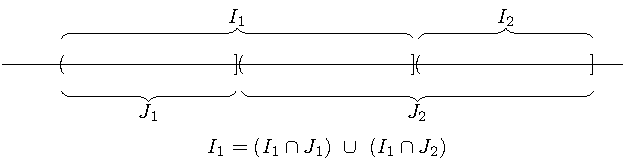
\includegraphics[scale=0.8]{figures/premeasure-on-algebra-of-h-ints/main.pdf}
                \caption{Illustration of interval intersections between $I_1$, $I_2$, and $J_1$, $J_2$.}
                \label{fig:interval_union}
            \end{figure}
            (\textit{See Figure 2.1 as a motivating example}). Apply the special case inside each $I_i$ and $J_j$:
                \begin{equation*}
                \begin{split}
                    \mu_0(I_i) = \sum_{j = 1}^n \mu_0 (I_i \cap J_j), \h9\h4 \mu_0(J_j) = \sum_{i = 1}^n \mu_0 (I_i \cap J_j).
                \end{split}
                \end{equation*}
            Summing each equation and rearranging gives $\sum_{i = 1}^n \mu_0(I_i) = \sum_{i,j}\mu_0 (I_i \cap J_j) = \sum_{j = 1}^n \mu_0(J_j)$. Thus $\mu_0$ is well-defined.

            We only need to show that $\mu_0$ satisfies countable additivity. Let $\{A_j\}_{j = 1}^\infty \subset \cA$ be a family of disjoint sets, where $\bigcup_{j = 1}^\infty A_j \in \cA$. Since everything in $\cA$ is a finite disjoint union of $h$-intervals, we can write:
                \begin{equation*}
                \begin{split}
                    \bigcup_{j = 1}^\infty A_j = \bigcup_{n = 1}^N I_n, \h9\h4 A_j = \bigcup_{i = 1}^{N_j}I_{i,j}.
                \end{split}
                \end{equation*}
            But observe that:
                \begin{equation*}
                \begin{split}
                    I_n 
                    & = I_n \cap  \left(\bigcup_{j = 1}^\infty A_j \right)\\
                    & = \bigcup_{j = 1}^\infty (I_n \cap A_j) \\
                    & = \bigcup_{j = 1}^\infty \left( I_n \cap \left( \bigcup_{i = 1}^{N_j}I_{i,j}\right) \right) \\
                    & = \bigcup_{j = 1}^\infty \bigcup_{i = 1}^{N_j} (I_n \cap I_{i,j}).
                \end{split}
                \end{equation*}
            It is enough to assume that if an $h$-interval $I$ is a countable disjoint union of $h$-intervals $\{I_j\}_{j = 1}^\infty$, then $\mu_0(I) = \sum_{j = 1}^\infty \mu_0(I_j)$. Let $I = (a,b]$ and $I_j = (a_j,b_j]$. One direction of the equality can be seen as folllows:
                \begin{equation*}
                \begin{split}
                    \mu_0(I) 
                    & = \mu_0\left(\bigcup_{j = 1}^n I_j\right) + \mu_0\left(I \setminus \bigcup_{j = 1}^n I_j\right) \\
                    & \geq \mu_0 \left( \bigcup_{j = 1}^n I_j \right) \\
                    & = \sum_{j = 1}^n \mu_0(I_j).
                \end{split}
                \end{equation*}
            Taking $n \rightarrow \infty$ gives $\mu_0(I) \geq \sum_{j = 1}^\infty \mu_0(I_j)$. Conversely, let $\epsilon > 0$. By the right-continuity of $F$, choose $\delta > 0$ such that $F(a + \delta) - F(a) < \epsilon$. Similarly, choose $\delta_j > 0$ such that $F(b_j + \delta_j) - F(b_j) < \frac{\epsilon}{2^j}$. Then the compact set $[a+\delta,b]$ is covered by the open intervals $\{(a_j,b_j + \delta_j\}_{j = 1}^\infty $, so there exists a finite subcover $\{ (a_j,b_j]\}_{j = 1}^N$. Without loss of generality, let $a_1 < a_2 < ... < a_N$. By construction $b_j + \delta_j \in (a_{j + 1}, b_{j+1} + \delta_{j+1})$. We then get:
                \begin{equation*}
                \begin{split}
                    \mu_0(I)
                    & = F(b) - F(a) \\
                    & \leq F(b) - F(a+\delta) + \epsilon \\
                    & = F(b_N + \delta_N) - F(a_N) + \sum_{j = 1}^{N-1} \bigl(F(a_{j+1}) - F(a_j)\bigr) + \epsilon \\
                    & \leq F(b_N + \delta_N) - F(a_N) + \sum_{j = 1}^{N-1} \bigl(F(b_j + \delta_j) - F(a_j)\bigr) + \epsilon \\
                    & = \sum_{j = 1}^{N} \bigl(F(b_j + \delta_j) - F(a_j)\bigr) + \epsilon \\
                    & < \sum_{j = 1}^{N} \bigl(F(b_j) + \frac{\epsilon}{2^j} - F(a_j)\bigr) + \epsilon \\
                    & \leq \sum_{j = 1}^N \bigl(F(b_j) - F(a_j)\bigr) + 2 \epsilon \\
                    & = \sum_{j = 1}^N \mu_0(I_j) + 2 \epsilon \\
                \end{split}
                \end{equation*}
            Taking $\epsilon \rightarrow 0$ finally shows that $\mu_0$ is countable additive over disjoint unions of $h$-intervals. Thus, $\mu_0$ is a well-defined premeasure defined on $\cA$, the algebra of countable disjoint unions of $h$-intervals.
        \end{proof}

    Having finally constructed the premeasure $(\bfR, \cA, \mu_0)$, we can now apply \nameref{thm:premeasure}.

    \begin{theorem}
        Let $F$ be a distribution function. There is a unique Borel measure $\mu_F$ on $\bfR$ such that $\mu_F((a,b]) = F(b) - F(a)$. If $G$ is another such function, then $\mu_F = \mu_G$ if and only if $F-G$ is constant. Conversely, if $\mu$ is a Borel measure on $\bfR$ that is finite on all bounded Borel sets, define:
            \begin{equation*}
            \begin{split}
                F(x) =
                \begin{cases}
                    \mu ( (0,x]), & x > 0, \\
                    0, & x = 0, \\
                    \mu ( -(x,0]), & x < 0, \\
                \end{cases}
            \end{split}
            \end{equation*}
        Then $F$ is a distribution, and $\mu = \mu_F$.
    \end{theorem}
        \begin{proof}
            Proposition~\ref{prop:premeasures-well-defined} showed that each $F$ induces a premeasure on $\cA$, the collection of countable disjoint unions of $h$-intervals. It is clear that $F$ and $G$ induce the same premeasure if $F-G$ is constant, and that these premeasures are $\sigma$-finite. The assertion that there is a \textui{unique} Borel measure comes from \nameref{thm:premeasure}. Given the outer measure $\mu^\ast$, induced by the premeasure on countable disjoint unions of $h$-intervals, define $\mu_F := \restr{\mu^\ast}{\fM(\cA)} = \restr{\mu^\ast}{\cB_\bfR}$. The converse direction follows from the monotonicity of $\mu$.
        \end{proof}

    There are many levels to this application of Theorem~\ref{thm:caratheodory}, Theorem~\ref{thm:premeasure}, and Proposition~\ref{prop:premeasures-well-defined}. Different restrictions of the outer-measure space $(X,\cP(X),\mu^\ast)$ give different $\sigma$-algebra to work in. We have the chain of $\sigma$-algebras:
        \begin{equation*}
        \begin{split}
            \cA \subset \cB_\bfR \subsetneq \cM^\ast \subset \cP(X),
        \end{split}
        \end{equation*}
    Where $\mu_F := \restr{\mu^\ast}{\fM(\cA)} = \restr{\mu^\ast}{\cB_\bfR}$ is the measure on $\cB_\bfR$, and $\restr{\mu^\ast}{\cM^\ast}$ is the \textui{complete} measure on $\cM^\ast$, the set of all $\mu^\ast$-measurable sets. One can rigorously show that the domain of $\restr{\mu^\ast}{\cM^\ast}$ is strictly larger than the domain of $\restr{\mu^\ast}{\cB_\bfR}$.

    \begin{definition}
        Let $\mu_0$ be a premeasure on $\cA$ (the algebra of countable disjoint unions of $h$-intervals) and $F$ a distribution function on $\mu_0$. The restriction of the $(X,\cA,\mu_0)$ induced outer measure onto all measurable sets is called the \textui{Lebesgue-Stieltjes measure associated to F}.
    \end{definition}\phantom{a}\nl
    
    \noindent For the remainder of this section, let $\mu$ denote the Lebesgue-Stieltjes measure on $\bfR$ associated to the distribution function $F$, $\cM_\mu$ the domain of $\mu$, and $\cA$ the algebra of countable disjoint unions of $h$-intervals. We can rewrite our standard definition of the outer measure as follows:
        \begin{equation*}
        \begin{split}
            \mu(E) 
            & = \inf\left\{ \sum_{j = 1}^\infty \mu_0(A_j) \mid \{A_j\}_{j = 1}^\infty \subset \cA, \bigcup_{j = 1}^\infty A_j \supset E\right\} \\
            & = \inf \left\{ \sum_{j = 1}^\infty \mu \bigl((a_j,b_j]\bigr) \mid  \{(a_j,b_j]\}_{j = 1}^\infty \subset \cA, \bigcup_{j = 1}^\infty (a_j,b_j] \supset E\right\}.
        \end{split}
        \end{equation*}
    Note that $\restr{\mu}{\cA} = \mu_0$, hence the second equality.

    \begin{theorem}\label{thm:measurable-sets-prop}
        If $E \in \cM_\mu$, then:
        \begin{enumerate}[label = (\arabic*),itemsep=1pt,topsep=3pt]
            \item $\mu(E) = \inf\{\mu(U) \mid U \supset E \text{ and }U \text{ is open }\} $.
            \item $\mu(E) = \sup\{\mu(K) \mid K \subset E \text{ and }K \text{ is compact }\}$.
        \end{enumerate}
    \end{theorem}
        \begin{proof}
            (1) Note that $\mu(E) \leq \inf \{\mu(U) \mid U \supset E \text{ and }U \text{ is open }\}$ follows by monotonicity since $E \subset U$. For the other direction, let $\epsilon > 0$. Choose $h$-intervals $\{I_j\}_{j = 1}^\infty := \{(a_j,b_j]\}_{j = 1}^\infty \subset \cA$ such that $\bigcup_{j = 1}^\infty I_j \supset E$ and:
                \begin{equation*}
                \begin{split}
                    \mu(E) + \epsilon \geq \sum_{j = 1}^\infty \mu(I_j).
                \end{split}
                \end{equation*}
            By the right continuity of $F$ (our underlying distribution function), for each $j$ choose $\delta_j > 0$ such that $F(b_j + \delta_j) - F(b_j) < \frac{\epsilon}{2^j}$. Observe that:
                \begin{equation*}
                \begin{split}
                    \mu(E) + \epsilon 
                    & \geq \sum_{j = 1}^\infty \mu(I_j) \\
                    & = \sum_{j = 1}^\infty \mu \Bigl((a_j,b_j + \delta_j) \setminus (b_j, b_j + \delta_j)\Bigr) \\
                    & = \sum_{j=1}^\infty \Bigl(\mu\bigl((a_j, b_j + \delta_j)\bigr) - \mu\bigl((b_j, b_j + \delta_j)\bigr)\Bigr) \\
                    & \geq \sum_{j=1}^\infty \Bigl(\mu\bigl((a_j, b_j + \delta_j)\bigr) - \mu\bigl((b_j, b_j + \delta_j]\bigr)\Bigr) \h9\h9\text{\tiny Threw in endpoint, hence the inequality} \\
                    & \geq \sum_{j=1}^\infty \Bigl(\mu\bigl((a_j, b_j + \delta_j)\bigr) - \bigl(F(b_j + \delta_j) - F(b_j)\bigr)\Bigr) \\
                    & \geq \sum_{j=1}^\infty \Bigl(\mu\bigl((a_j, b_j + \delta_j)\bigr) - \frac{\epsilon}{2^j}\Bigr) \\
                    & = \sum_{j=1}^\infty \Bigl(\mu\bigl((a_j, b_j + \delta_j)\bigr)\Bigr) - \epsilon \\
                    & \geq \mu \left( \bigcup_{j = 1}^\infty (a_j,b_j + \delta_j) \right) - \epsilon
                \end{split}
                \end{equation*}
            Take $U_\epsilon := \bigcup_{j = 1}^\infty (a_j,b_j + \delta_j)$. Then $\mu(E) \geq \mu(U_\epsilon) + \epsilon$. Taking $\epsilon \rightarrow \infty$ gives the desired result.

            (2) We proceed by cases on $E$. Case 1: $E$ is bounded.  Apply part (1) to the set $\overline{E} \setminus E$. Let $\epsilon > 0$. Find an open set $U \supset \overline{E} \setminus E$ such that $\mu(U) - \mu(\overline{E} \setminus E) \leq \epsilon$. Define $K = \overline{E} \setminus U$. Note that $K$ is bounded since $\overline{E} \setminus U = \overline{E} \cap U^c$ is a closed subset of $\overline{E}$, which is a compact set. We can write:
                \begin{equation*}
                \begin{split}
                    K 
                    & = \overline{E} \setminus U \\
                    & = \bigl(E \cup (\overline{E} \setminus E)\bigr) \setminus U \\
                    & = E \setminus U \\
                    & \subset E.
                \end{split}
                \end{equation*}
            Note that $E \setminus K \subset U \setminus (\overline{E} \setminus E)$ {\color{red}* (the dotted line apparently)}. So $\mu(E \setminus K) \leq \mu(U \setminus (\overline{E} \setminus E))$, which is equivalent to $\mu(E) - \mu(K) \leq \mu(E) - \mu(\overline{E} \setminus E) \leq \epsilon$. Rearranging and taking $\epsilon \rightarrow 0$ gives $\mu(E) \leq \mu(K)$, which implies $\mu(E) \leq \sup \{\mu(K) \mid K \subset E \text{ and } K \text{ is compact }\}$. The reverse direction is obvious by monotonicty.

            Case 2: $E$ is unbounded. Again, one direction is obvious by monotonicity. Let $E_j = E \cap (j,j+1]$. Then $\mu(E) = \sum_{j = 1}^\infty \mu(E_j)$. For all $j$, let $K_j \subset E_j$ be compact, and:
                \begin{equation*}
                \begin{split}
                    \mu(E) - \mu(K_j) < \frac{\epsilon}{2^{|j|}}.
                \end{split}
                \end{equation*}
            Then:
                \begin{equation*}
                \begin{split}
                    \mu(E_j) 
                    & = \sum_{j \in \bfZ}\mu(E_j) \\
                    & \leq \sum_{j = -\infty}^\infty \left( \mu(K_j) + \frac{\epsilon}{2^{|j|}} \right) \\
                    & = 3\epsilon + \sum_{j = -\infty}^\infty \mu(K_j) \\
                    & = 3\epsilon + \lim_{n \rightarrow \infty} \mu\left(\bigcup_{i = -n}^n K_i\right) \\
                \end{split}
                \end{equation*}
            Note that finite unions of compact sets is compact. Taking $\epsilon \rightarrow 0$ gives the desired result.
        \end{proof}

    \begin{theorem}
        Let $E \subset \bfR$ be of finite measure. The following are equivalent:
            \begin{enumerate}[label = (\arabic*),itemsep=1pt,topsep=3pt]
                \item $E \in \cM_\mu$;
                \item $E = V \setminus N_1$, where $V$ is a $G_\delta$ set and $\mu(N_1) = 0$.
                \item $E = H \cup N_2$, where $H$ is an $F_\sigma$ set and $\mu(N_2) = 0$.
            \end{enumerate}
    \end{theorem}
        \begin{proof}
            (1)$\Rightarrow$(2) Let $E \in \cM_\mu$. By Theorem~\ref{thm:measurable-sets-prop}, there exists open sets $\{U_n\}_{n \in \bfN}$ such that:
                \begin{equation*}
                \begin{split}
                    \mu(U_n)  < \mu(E) + \frac{1}{2^n}. 
                \end{split}
                \end{equation*}
            Since $\mu(E) < \infty$, we can write this as $\mu(U_n)  - \mu(E) < \frac{1}{2^n}$. Consider the $G_\delta$ set $\bigcap_{n = 1}^\infty U_n$. Since $E \subset U_n$ for all $n \in \bfN$, surely $E \subset \bigcap_{n = 1}^\infty U_n$. By the monotonicity of $\mu$, we have $\mu(E) \leq \mu \left( \bigcap_{i = 1}^n U_n \right)$. Hence:
                \begin{equation*}
                \begin{split}
                    \mu(E) \leq \mu \left( \bigcap_{i = 1}^\infty U_n \right) \leq \mu(U_n) \leq \mu(E) + \frac{1}{2^n}.
                \end{split}
                \end{equation*}
            Taking $n \rightarrow \infty$ gives $\mu \left( \bigcap_{n = 1}^\infty U_n \right) = \mu(E)$, which is equivalent to $\mu \left( \bigcap_{n = 1}^\infty U_n \setminus E \right) = 0$. Take $N_1 := \bigcap_{n = 1}^\infty U_n \setminus E$ and $V = \bigcap_{n = 1}^\infty U_n$. Then $E = V \cap N_1$, where $V$ is a $G_\delta$ set and $\mu(N_1) = 0$.

            (1)$\Rightarrow$(3). Let $E \in \cM_\mu$. By Theorem~\ref{thm:measurable-sets-prop}, there exists compact sets $\{K_n\}_{n \in \bfN}$ such that:
                \begin{equation*}
                \begin{split}
                    \mu(E) - \frac{1}{2^n} < \mu(K_n).
                \end{split}
                \end{equation*}
            Define $H = \bigcup_{n \in \bfN}K_n$. Then $H$ is a $F_\sigma$ set. Since $K_n \subset E$ for all $n \in \bfN$, we have $H \subset E$. By monotonicity, we have $\mu(H) \leq \mu(E)$. But we also have:
                \begin{equation*}
                \begin{split}
                    \mu(E) - \frac{1}{2^n} < \mu(K_n) \leq \mu(H).
                \end{split}
                \end{equation*}
            Taking $n\rightarrow \infty$ gives $\mu(E) \leq \mu(H)$. Together, $\mu(E) = \mu(H)$; i.e., $\mu(E \setminus H) = 0$. Define $N_2 = E \setminus H$. Then $E = H \cup N_2$, where $H$ is an $F_\sigma$ set and $N_2$ is a null-set.

            (2)$\Rightarrow$(1) Suppose $E = V \setminus N_1$, where $V$ is a $G_\delta$ set and $N_1$ is a null-set. Since $V$ is a $G_\delta$ set, $V \in \cM_\mu$. Since $N_1$ is a null-set, it is measurable. Since $\cM_\mu$ is a 

            (3)$\Rightarrow$(1) This follows similarly as above.
        \end{proof}
    
    Since the countable union of $G_\delta$ sets may not be a $G_\delta$ set, it is not straight forward to use the fact $\mu$ is $\sigma$-finite to extend the result for sets of finite measures to the general case. In fact, proving the general case is more like re-doing the proof completely than simply extending the result for sets of finite measures.

    \begin{proposition}\label{prop:approximate-leb-stielt-meas-sets-with-finite-union-of-open-ints}
        If $E \in \cM_\mu$ and $\mu(E) < \infty$, then for every $\epsilon > 0$ there is a set $A$ that is a finite union of open intervals such that $\mu(E \triangle A) < \epsilon$.
    \end{proposition}
        \begin{proof}
            Since $E \in \cM_u$, $\mu(E) = \inf\{\mu(U) \mid U \supset E \text{ and } U \text{ is open }\}$. Let $\epsilon > 0$. Find an open set $U$ such that $U \supset E$ and:
                \begin{equation*}
                \begin{split}
                    \mu(U) < \mu(E) + \frac{\epsilon}{2}.
                \end{split}
                \end{equation*}
            Since $U$ is open, there exists disjoint open intervals $\{U_j\}_{j = 1}^\infty$ such that $\bigcup_{j = 1}^\infty U_j = U$. It follows that:
                \begin{equation*}
                \begin{split}
                    \mu(U) 
                    & = \mu \left( \bigcup_{j = 1}^\infty U_j \right) \\
                    & = \sum_{j = 1}^\infty \mu(U_j).
                \end{split}
                \end{equation*}
            Note that this series converges since $\mu(U) < \mu(E) + \frac{\epsilon}{2}$. Pick $N$ large so that:
                \begin{equation*}
                \begin{split}
                    \sum_{j = 1}^{N-1}\mu(U_j) < \frac{\epsilon}{2}.
                \end{split}
                \end{equation*}
            Define $A = \bigcup_{j = 1}^{N-1}$. Then $A \subset U$. Observe that:
                \begin{equation*}
                \begin{split}
                    \mu(E \triangle A)
                    & = \mu\bigl((E \setminus A) \cup (A \setminus E)\bigr) \\
                    & \leq \mu \bigl(\bigr)
                \end{split}
                \end{equation*}
            {\color{red} should finish} 
        \end{proof}

    We will now start discussing the most important measure on $\bfR$.

    \begin{definition}
        The Lebesgue-Stieltjes measure on $\bfR$ associated to the distribution function $F(x) = x$ is called the \textui{Lebesgue measure on $\bfR$}, and is denoted by $m$. The domain of $m$ is the collection of $\mu^\ast$-measurable sets, which we will denote as $\cL$.
    \end{definition}

    Sometimes we may also refer to the domain of $\restr{\mu^\ast}{\cB_\bfR}$ as the Lebesgue measure. This will get confusing at times.

    \begin{theorem}
        Let $E \in \cL$. For all $s,r \in \bfR$, we have $E+s \in \cL$ and $rE \in \cL$. Moreover, $m(E +s) = m(E)$ and $m(rE) = |r|m(E)$.
    \end{theorem}
        \begin{proof}
            Every open set in $\bfR$ can be expressed as the \textui{countable} union of disjoint open intervals. {\color{red} ...}
        \end{proof}

\iffalse
\section*{\centering Exercises}
    \addcontentsline{toc}{section}{\protect\numberline{}Exercises}
\begin{exercise}
Let $\cA \subset \cP(X)$ be an algebra, $\cA_\sigma$ the collection of countable unions of sets in $\cA$, and $\cA_{\sigma\delta}$ the collection of countable intersections of sets in $\cA_\sigma$. Let $\mu_0$ be a premeasure on $\cA$ and $\mu^\ast$ the induced outer measure.
    \begin{enumerate}[label = (\alph*),itemsep=1pt,topsep=3pt]
        \item For any $E \subset X$ and $\epsilon > 0$ there exists $A \in \cA_\sigma$ with $E \subset A$ and $\mu^\ast(A) \leq \mu^\ast(E) + \epsilon$.
        \item If $\mu^\ast(E) < \infty$, then $E$ is $\mu^\ast$-measurable if and only if there exists $B \in \cA_{\sigma\delta}$ with $E \subset B$ and $\mu^\ast(B \setminus E) = 0$.
        \item If $\mu_0$ is $\sigma$-finite, the restriction $\mu^\ast(E) < \infty$ in (b) is superfluous.
    \end{enumerate}
\end{exercise}
    \begin{proof}
        (a) Let $E \subset X$ and $\epsilon > 0$. By the defintion of $\mu^\ast(E)$, we can find $\{A_j\}_{j = 1}^\infty \subset \cA$ such that $\bigcup_{j = 1}^\infty A_j \supset E$ and: 
            \begin{equation*}
            \begin{split}
                \mu^\ast(E) + \epsilon 
                & \geq \sum_{j = 1}^\infty \mu_0(A_j) \h9\h9\h8\text{\tiny Property of infimums}\\ 
                & = \sum_{j = 1}^\infty \mu^\ast (A_j) \h9\h9\h9 \text{\tiny Because $\restr{\mu^\ast}{\cA} = \mu_0$}\\
                & \geq \mu^\ast \left( \bigcup_{j = 1}^\infty A_j \right). \h9\h9\h1\text{\tiny Outer measures are subadditive}
            \end{split}
            \end{equation*}

        (b) ($\Rightarrow$) Suppose $E$ is $\mu^\ast$-measurable. By part (a), for each $n \in \bfN$, there exists $\{A_n\}_{n \in \bfN} \subset \cA_\sigma$ such that $E \subset A_n$ and:
            \begin{equation*}
            \begin{split}
                \mu^\ast(A_n) \leq \mu^\ast(E) + \frac{1}{n}.
            \end{split}
            \end{equation*}
        Since $\mu^\ast(E) < \infty$, we can rearrange the above inequality as:
            \begin{equation*}
            \begin{split}
                \mu^\ast(A_n) - \mu^\ast(E) \leq \frac{1}{n}.
            \end{split}
            \end{equation*}
        Define $B := \bigcap_{n \in \bfN}A_n \in \cA_{\sigma\delta}$. Observe that:
            \begin{equation*}
            \begin{split}
                \mu^\ast(B \setminus E)
                & = \mu^\ast(B \cap E^c) \\
                & \leq \mu^\ast (A_n \cap E^c) \h9\h9\h9\h9
                \h9\h9\text{\tiny Monotonicity \& $B \subset A_n$ $\forall n$}\\
                & = \mu^\ast(A_n) - \mu^\ast(A_n \cap E) \h9\h9\text{\tiny Since $E$ is $\mu^\ast$-measurable} \\
                & = \mu^\ast(A_n) - \mu^\ast(E) \h9\h9\h9\h9\h8 \text{\tiny Since $E \subset A_n$}\\
                & \leq \frac{1}{n} 
            \end{split}
            \end{equation*}
        Hence $\mu^\ast(B \setminus E) = 0$. 

        ($\Leftarrow$) Suppose there exists $B \in \cA_{\sigma \delta}$ such that $E \subset B$ and $\mu^\ast(B \setminus E) = 0$. Apply part (a) to the set $B \setminus E$. For each $n \in \bfN$, there exists $\{A_n\}_{n \in \bfN} \subset \cA_\sigma$ such that $B \setminus E \subset A_n$ and :
            \begin{equation*}
            \begin{split}
                \mu^\ast(A_n) 
                & \leq \mu^\ast(B \setminus E) + \frac{1}{n} \\
                & = \frac{1}{n}.
            \end{split}
            \end{equation*}
        Note that $\bigcap_{n \in \bfN}A_n \in \cA_{\sigma\delta} \subset \cM^\ast$, hence it is measurable. Similarly, $B \in \cA_{\sigma\delta} \subset \cM^\ast$ is measurable. Since $B \setminus E \subset A_n$ for each $n \in \bfN$, we have $B \setminus E \subset \bigcap_{n \in \bfN}A_n$. By monotonicity, observe that:
            \begin{equation*}
            \begin{split}
                \mu^\ast \left( \bigcap_{n \in \bfN}A_n \right) \leq \mu^\ast(A_n) \leq \frac{1}{n}.
            \end{split}
            \end{equation*}
        Since this holds true for all $n \in \bfN$, we have that $\bigcap_{n \in \bfN}A_n$ is a null-set. Since $\cM^\ast$ is complete, every subset of a null-set is measurable, hence $B \setminus E \subset \bigcap_{n \in \bfN}A_n$ is measurable. We can now write:
            \begin{equation*}
            \begin{split}
                E = B \setminus (B \setminus E) = B \cap (B \setminus E)^c.
            \end{split}
            \end{equation*}
        Since $\cM^\ast$ is a $\sigma$-algebra, and since $E$ is the countable intersection of measurable sets (note that $(B\setminus E)^c$ is measurable since $B\setminus E$ is measurable), we have that $E$ is measurable.

        (c) We did not use the restriction $\mu^\ast (E) < \infty$ in the ($\Leftarrow$) direction, hence we only need to prove ($\Rightarrow$) for when $\mu_0$ is $\sigma$-finite. Let $X = \bigcup_{j = 1}^\infty X_j$. Then $\mu_0(X_i) < \infty$. Define $E_n = E \cap \left( \bigcup_{j = 1}^n X_j \right)$. Then $\bigcup_{n = 1}^\infty E_n = E$. \nl
        
        \noindent For every $n \in \bfN$, apply part (a) to $E_n$. \nl
        
        \noindent There exists $C_n \in \cA_\delta$ such that $E_n \subset C_n$ and $\mu^\ast(C_n) \leq \mu^\ast(E_n) + \frac{1}{n}$. Define $C = \bigcap_{n = 1}^\infty C_n$. Then $\mu^\ast(C) \leq \mu^\ast(C_n) \leq \mu^\ast(E_n) + \frac{1}{n}$. Rearranging gives $\mu^\ast(C) - \mu^\ast(E_n) \leq \frac{1}{n}$. But since $\mu^\ast(E_n) \leq \mu^\ast(E)$, we have $\mu^\ast(C) - \mu^\ast(E) \leq \mu^\ast(C) - \mu^\ast(E_n) \leq \frac{1}{n}$. Since this holds true for all $n \in \bfN$, we have $\mu^\ast(C \setminus E) = 0$.
    \end{proof}
%%%%%%%%%%%%%%%%%%%%%%%%%%%%%%%%%%%%%%%%%%%%%%%%%%
\begin{exercise}
    Let $\mu^\ast$ be an outer measure on $X$ induced by the finite premeasure $\mu_0$. If $E \subset X$, define the \textui{inner measure} of $E$ to be $\mu_\ast(E) = \mu_0(X) - \mu^\ast(E^c)$. Show $E$ is $\mu^\ast$-measurable if and only if $\mu^\ast(E) = \mu_\ast(E)$.
\end{exercise}
    \begin{proof}
        ($\Rightarrow$) Suppose $E$ is $\mu^\ast$-measurable. Then $E^c$ is also $\mu^\ast$-measurable since $\cM^\ast$ is a $\sigma$-algebra. We can write:
            \begin{equation*}
            \begin{split}
                \mu^\ast (X) = \mu^\ast(E) + \mu^\ast(E^c).
            \end{split}
            \end{equation*}
        Since $X\in \cA$ and $\mu_0 = \restr{\mu^\ast}{\cA}$, we have:
            \begin{equation*}
            \begin{split}
                \mu_0(X) = \mu^\ast(E) + \mu^\ast(E^c).
            \end{split}
            \end{equation*}
        Subtracting both sides by $\mu^\ast(E^C)$ gives $\mu_\ast(E) = \mu^\ast(E)$. 

        ($\Leftarrow$) Now suppose $\mu^\ast(E) = \mu_0(X) - \mu^\ast(E^c)$. Again, since $X\in \cA$ and $\mu_0 = \restr{\mu^\ast}{\cA}$, we have:
            \begin{equation*}
            \begin{split}
                \mu^\ast(E) + \mu^\ast(E^c) = \mu^\ast(X) = \mu_0(X) < \infty
            \end{split}
            \end{equation*}
        For each $n \in \bfN$, Apply Exercise 1, part (a) to $E$. Then there exists $A_n \in \cA_\sigma$ such that $E \subset A_n$ and $\mu^\ast(A_n) \leq \mu^\ast(E) + \frac{1}{n}$. Define $B := \bigcap_{n = 1}^\infty A_n$. Note that $B$ is measurable since $B \in \cA_{\sigma\delta} \subset \cM^\ast$. Moreover since $E \subset A_n$ for all $n \in \bfN$, we have $E \subset B$. Together:
            \begin{equation*}
            \begin{split}
                \mu^\ast(E) \leq \mu^\ast(B) \leq \mu^\ast(A_n) \leq \mu^\ast(E) + \frac{1}{n}.
            \end{split}
            \end{equation*}
        Since this holds true for all $n \in \bfN$, it must be that $\mu^\ast(E) = \mu^\ast(B)$. Quickly note:
            \begin{equation*}
            \begin{split}
                \mu^\ast(B) + \mu^\ast(B^c) 
                & = \mu^\ast(X) \\
                & = \mu^\ast(E) + \mu^\ast(E^c).
            \end{split}
            \end{equation*}
        Since $\mu^\ast(B) = \mu^\ast(E) < \infty$, we have $\mu^\ast(E^c) = \mu^\ast(B^c)$. Now by the measurability of $B$:
            \begin{equation*}
            \begin{split}
                \mu^\ast (E) + \mu^\ast(E^c) 
                & = \mu^\ast(E) + \mu^\ast(E^c \cap B) + \mu^\ast(E^c \cap B^c) \\
                & = \mu^\ast(E) + \mu^\ast(E^c \cap B) + \mu^\ast(B^c) \\
                & = \mu^\ast(E) + \mu^\ast(E^c \cap B) + \mu^\ast(E^c) \\
            \end{split}
            \end{equation*}
        Hence $\mu^\ast(E^c \cap B) = \mu^\ast(B \setminus E) = 0$. By Exercise 1, part (b), $E$ is $\mu^\ast$-measurable.
    \end{proof}

    \begin{exercise}
        If $E \in \cM_\mu$ and $\mu(E) < \infty$, then for every $\epsilon > 0$ there is a set $A$ that is a finite union of open intervals such that $\mu(E \triangle A) < \epsilon$.
    \end{exercise}
        \begin{proof}
            Since $E \in \cM_u$, $\mu(E) = \inf\{\mu(U) \mid U \supset E \text{ and } U \text{ is open }\}$. Let $\epsilon > 0$. Find an open set $U$ such that $U \supset E$ and:
                \begin{equation*}
                \begin{split}
                    \mu(U) < \mu(E) + \frac{\epsilon}{2}.
                \end{split}
                \end{equation*}
            Since $U$ is open, there exists disjoint open intervals $\{U_j\}_{j = 1}^\infty$ such that $\bigcup_{j = 1}^\infty U_j = U$. It follows that:
                \begin{equation*}
                \begin{split}
                    \mu(U) 
                    & = \mu \left( \bigcup_{j = 1}^\infty U_j \right) \\
                    & = \sum_{j = 1}^\infty \mu(U_j).
                \end{split}
                \end{equation*}
            Note that this series converges since $\mu(U) < \mu(E) + \frac{\epsilon}{2}$. Pick $N$ large so that:
                \begin{equation*}
                \begin{split}
                    \sum_{j = 1}^{N-1}\mu(U_j) < \frac{\epsilon}{2}.
                \end{split}
                \end{equation*}
            Define $A = \bigcup_{j = 1}^{N-1}$. Then $A \subset U$. Observe that:
                \begin{equation*}
                \begin{split}
                    \mu(E \triangle A)
                    & = \mu\bigl((E \setminus A) \cup (A \setminus E)\bigr) \\
                    & \leq \mu \bigl(\bigr)
                \end{split}
                \end{equation*}
        \end{proof}
\fi
    \chapter{Integration}

Having studied measure spaces, we turn out attention to maps between them.

\section{Measurable Functions}

\begin{definition}
    Let $X$ be a set and $\cM$ a $\sigma$-algebra on $X$. We call the pair $(X,\cM)$ a \textui{measurable space}.
\end{definition}

Note that a \textit{measure space} has a measure associated to it.

\begin{definition}
    Let $(X,\cM)$ and $(Y,\cN)$ be measurable spaces. A function $f:X \rightarrow Y$ is said to be \textui{$(\cM,\cN)$-measurable} if for every $E \in \cN$, we have $f^{-1}(E) \in \cM$.
\end{definition}

\begin{proposition}\label{prop:measurable-functs}
    \phantom{a}
    \begin{enumerate}[label = (\arabic*),itemsep=1pt,topsep=3pt]
        \item If $f:X \rightarrow Y$ is $(\cM,\cN)$-measurable and $g:Y \rightarrow Z$ is $(\cN,\cO)$-measurable, then $g \circ f :X \rightarrow Z$ is $(\cM,\cO)$-measurable.
        
        \item Let $\cE$ be a set and suppose $(X,\cM)$ and $(Y,\fM(\cE))$ are measurable spaces. A function $f:X \rightarrow Y$ is $(\cM,\fM(\cE))$-measurable if and only if for every $E \in \cE$ we have $f^{-1}(E) \in \cM$
        
        \item Let $X,Y$ be metric spaces. If $f:X\rightarrow Y$ is continuous, then $f$ is $(\cB_X,\cB_Y)$-measurable.
        
        \item Let $(Y_1,\cN_1)$ and $(Y_2,\cN_2)$ be measurable spaces. The projection maps:
            \begin{equation*}
            \begin{split}
                Y_1 \times Y_2 \xrightarrow{\pi_i}Y_i, \h6 i=1,2
            \end{split}
            \end{equation*}
        are $(\cN_1 \otimes \cN_2,\cN_i)$-measurable.

        \item The function $f:X \rightarrow Y_1 \times Y_2$ is $(\cM,\cN_1 \otimes \cN_2)$-measurable if and only if $\pi_1 \circ f$ is $(\cM,\cN_1)$-measurable and $\pi_2 \circ f$ is $(\cM,\cN_2)$-measurable.
    \end{enumerate}
\end{proposition}

We will be focusing on measurable functions whose codomain is a metric space, hence the following definition.

\begin{definition}
    \phantom{a}
    \begin{enumerate}[label = (\arabic*),itemsep=1pt,topsep=3pt]
        \item Let $(X,\cM)$ be a measurable space and $Y$ a metric space. A function $f:X \rightarrow Y$ is called \textui{$\cM$-measurable} if it is $(\cM,\cB_Y)$-measurable.
        \item A function $f:\bfR \rightarrow \bfR$ is called \textui{Lebesgue measurable} if it is $(\cL,\cB_\bfR)$-measurable.
    \end{enumerate}
\end{definition}

\begin{remark}
    Note that the composition of two Lebesgue measurable functions is \textit{not} Lebesgue measurable. If $f:\bfR \rightarrow \bfR$ and $g:\bfR \rightarrow \bfR$ are both Lebesgue measurable, then their composition $g \circ f$ is $(\cB_\bfR,\cB_\bfR)$-measurable by Proposition~\ref{prop:measurable-functs}.
\end{remark}

\begin{proposition}
    Let $(X,\cM)$ be a measurable space and $f:X \rightarrow \bfC$ a map. Then $f$ is $\cM$-measurable if and only if $\fR(f)$ and $\fI(f)$ are $\cM$-measurable.
\end{proposition}
    \begin{proof}
        Recall from Proposition~\ref{} that $\cB_\bfC = \cB_{\bfR^2} = \cB_\bfR \otimes \cB_\bfR$. Define $\Phi:\bfC \rightarrow \bfR^2$ by $a+bi \mapsto (a,b)$. Then $\Phi \circ f = (\fR(f),\fC(f))$. {\color{red} I don't understand this shit at all}
    \end{proof}

\begin{proposition}\label{prop:sums-prods-of-measurable-functions}
    If $f,g:X \rightarrow \bfR$ are both $\cM$-measurable, then $f+g$ and $fg$ are $\cM$-measurable.
\end{proposition}
    \begin{proof}
        Consider the composition of maps:
            \begin{equation*}
            \begin{split}
                X \xrightarrow{(f,g)} \bfR \times \bfR \xrightarrow{P} \bfR,
            \end{split}
            \end{equation*}
        where:
            \begin{equation*}
            \begin{split}
                (f,g)(x) = (f(x),g(x)), \h9 P(x,y) = x + y.
            \end{split}
            \end{equation*}
        It is well-known that $P$ is continuous, hence $P$ is $(\cB_{\bfR}\otimes\cB_{\bfR},\cB_\bfR)$-measurable. Moreover, $(f,g)$ is $(\cM,\cB_{\bfR}\otimes\cB_{\bfR})$-measurable because \textemdash by part (5) of Proposition~\ref{prop:measurable-functs} \textemdash we have $\pi_1 \circ (f,g) = f$ and $\pi_2 \circ (f,g) = g$. Then by part (1) of Proposition~\ref{prop:measurable-functs}, both $f$ and $g$ are $\cM$-measurable. The argument for $fg$ is identical.
    \end{proof}

A similar argument follows for when $f$ and $g$ are complex valued functions, however great care needs to be taken when considering functions whose codomain is the extended reals. It is tedious to avoid $\infty-\infty$.

\begin{proposition}
    Let $(X,\cM)$ be a measurable space. The following are equivalent:
        \begin{enumerate}[label = (\arabic*),itemsep=1pt,topsep=3pt]
            \item $f:X \rightarrow \bfR$ is $\cM$-measurable;
            \item For all $x \in \bfR$, $f^{-1}((a,\infty)) \in \cM$;
            \item For all $x \in \bfR$, $f^{-1}([a,\infty)) \in \cM$;
            \item For all $x \in \bfR$, $f^{-1}((-\infty,a)) \in \cM$;
            \item For all $x \in \bfR$, $f^{-1}((-\infty,a]) \in \cM$.
        \end{enumerate}
\end{proposition}
    \begin{proof}
        This follows from Proposition~\ref{prop:generators-of-borel} and part (2) of Proposition~\ref{prop:measurable-functs}.
    \end{proof}

{\color{red} Talk about borel sets of extended reals. Then explain that the above proposition but for extended real valued functions follows similarly, since you can show that borel sets of extended reals is generated by the closed endpoint rays.}

\newpage
\begin{proposition}\label{prop:limits-of-measurable-functions-are-measurable}
    Let $(X,\cM)$ be a measurable space and $(f_n)_{n = 1}^\infty$ be a sequence of functions in $\overline{\bfR}^X$ which are $\cM$-measurable for each $j \in \bfN$. The functions:
        \begin{equation*}
        \begin{split}
            \sup_n f_n, \h9 \inf_n f_n, \h9 \limsup_n f_n, \h9\liminf_n f_n
        \end{split}
        \end{equation*}
    are all $\cM$-measurable.
\end{proposition}
    \begin{proof}
        Define $h(x) := \sup\{f_n(x) \mid n \in \bfN\}$. We can see:
            \begin{equation*}
            \begin{split}
                x \in h^{-1}((a,\infty])
                & \iff h(x) > a \\
                & \iff \sup\{f_n(x) \mid n \in \bfN\} > a \\
                & \iff \exists j \in \bfN : f_j(x) > a \\
                & \iff \exists j \in \bfN : x \in f_j^{-1}((a,\infty]) \\
                & \iff x \in \bigcup_{j = 1}^\infty f_j^{-1}((a,\infty]).
            \end{split}
            \end{equation*}
        Hence $h^{-1}((a,\infty]) = \bigcup_{j = 1}^\infty f_j^{-1}((a,\infty])$. Note that $f_j^{-1}((a,\infty]) \in \cM$ for each $j \in \bfN$, and since $\cM$ is a $\sigma$-algebra this means $\bigcup_{j = 1}^\infty f_j^{-1}((a,\infty]) = h^{-1}((a,\infty])\in \cM$. Since $\{(a,\infty] \mid a \in \bfR\}$ generates $\cB_{\overline{\bfR}}$, by Proposition~\ref{prop:measurable-functs} we have that $\sup_n f_n$ is measurable.
    \end{proof}
\newpage
{\color{red} talk about why if its complex valued then its also measurable.}

\begin{proposition}
    If $f,g:X \rightarrow \overline{\bfR}$ are $\cM$-measurable, then $\max\{f,g\}$ and $\min\{f,g\}$ are $\cM$-measurable.
\end{proposition}
    {\color{red} \begin{proof}
        max and min can be expressed differnetly or smth like that
    \end{proof}}

\begin{definition}
    If $f:X \rightarrow \overline{\bfR}$, we define the \textui{positive} and \textui{negative parts} to be:
        \begin{equation*}
        \begin{split}
            f^+ = \max\{f,0\} \h1,\h9 f^- = \max \{-f,0\}.
        \end{split}
        \end{equation*}
\end{definition}

Note that $f = f^+ - f^-$, hence if  $f^+$ and $f^-$ are measurable, then $f$ is measurable.

\section{Lebesgue Integration}

We aim to generalize the Riemann integral. For the remainder of this section, fix a measure space $(X,\cM,\mu)$.

\begin{definition}
    The \textui{characteristic function} of a subset $E \subset X$ is defined as:
        \begin{equation*}
        \begin{split}
            \chi_E(x) = \begin{cases}
            1, & x\in E \\
            0, & x \not\in E.
            \end{cases} 
        \end{split}
        \end{equation*}
\end{definition}

\begin{proposition}
    Let $E \subset X$. Then $\chi_E$ is $\cM$-measurable if and only if $E \in \cM$.
\end{proposition}
    \begin{proof}
        ($\Rightarrow$) Note that $\{1\} \in \cB_\bfR$. Observe that:
            \begin{equation*}
            \begin{split}
                E
                & = \{x \mid \chi_E(x) = 1\} \\
                & = \{x \mid \chi_E(x) \in \{1\}\} \\
                & = \chi_E^{-1}(\{1\}).
            \end{split}
            \end{equation*}
        Since $\chi_E$ is $\cM$-measurable, $E \in \cM$.

        $(\Leftarrow)$ Since $E \in \cM$, by Proposition~\ref{prop:propoerties-of-sigma-algebras} $E \cup E^c = X \in \cM$. Let $A \in \cB_{\bfR}$ be arbitrary. Observe that:
            \begin{equation*}
            \begin{split}
                \chi_{E}^{-1}(A) 
                & = \chi_E^{-1}\bigl(A \cap \{0\}\bigr) \cup \chi_E^{-1}\bigl(A \cap \bfR\setminus\{0\}\bigr) \\
                & = \{x \mid \chi_E(x) = 0\} \cup \{x \mid \chi_E(x) \neq 0\} \\
                & = E^c \cup E \\
                & = X.
            \end{split}
            \end{equation*}
        Hence $\chi_E^{-1}(A) \in \cM$, giving that $\chi_E$ is $\cM$-measurable.
    \end{proof}

\begin{definition}
    \phantom{a}
    \begin{enumerate}[label = (\arabic*),itemsep=1pt,topsep=3pt]
        \item A \textui{simple-function} $\varphi$ is a finite linear combination of $\cM$-measurable characteristic functions.
        \item The \textui{standard representation} of a simple function $\varphi$ is:
            \begin{equation*}
            \begin{split}
                \varphi = \sum_{j = 1}^n z_j \chi_{E_j}, \text{ where } E_j = \varphi^{-1}(\{z_j\}) \text{ and }\Image \varphi = \{z_1,...,z_n\}.
            \end{split}
            \end{equation*}
    \end{enumerate}
\end{definition}

Note that the standard representation exhibits $\varphi$ as a linear combination of \textui{distinct coefficients}, as well as the $E_j$ forming a partition of $X$. It is clear that the set of all simple functions from $X$ to $\bfC$ is a $\bfC$-algebra.

\begin{theorem}\label{thm:increasing-sequence-of-simple-functions}
    Let $f:X \rightarrow [0,\infty]$ be $\cM$-measurable. There exists a sequence of simple functions $(\varphi_n)_n$ such that $0 \leq \varphi_1 \leq \varphi_2 \leq... \leq f$ and $\varphi_n \rightarrow f$. 
    \iffalse If $f$ is bounded, then this convergence is uniform.
    \fi
\end{theorem}
    \begin{proof}
        Define partitions of $[0,\infty]$ as follows: 
            \begin{equation*}
            \begin{split}
                I_n &:= (0,2^n],\\
                J_n &:= (2^n,\infty].\\
            \end{split}
            \end{equation*}
        Define partitions of $I_n$ as follows:
            \begin{equation*}
            \begin{split}
                I_n^k &:= \Bigl( \frac{k}{2^n},\frac{k+1}{2^n}\Bigr] \text{ for $k = 0,1,...,2^{2n}-1$}.
            \end{split}
            \end{equation*}
        Note that $f^{-1}(I_{n,k}), f^{-1}(J_n) \in \cM$ as $f$ is measurable. Moreover, $f^{-1}(I_{n,k})$ and $f^{-1}(J_n)$ partition $X$ as inverse images are well behaved with unions. Define:
            \begin{equation*}
            \begin{split}
                \varphi_n := \sum_{k = 0}^{2^{2n}-1} \left( \frac{k}{2^n} \chi_{f^{-1}(I_{n,k})} + 2^n \chi_{f^{-1}(J_n)} \right).
            \end{split}
            \end{equation*}
        This is a simple function. For any $x \in f^{-1}(I_{n,k})$, we have $\varphi_n(x) = \frac{k}{2^n} < f(x) \leq \frac{k+1}{2^n}$. Hence $0 < f(x) - \varphi_n(x) \leq \frac{k+1}{2^n}$. Sending $n \rightarrow \infty$ gives $\varphi_n \nearrow f$.
    \end{proof}

\begin{definition}
    The space of all measurable functions from $X$ to $[0,\infty]$ is denoted $L^+ := \{f:X \rightarrow [0,\infty] \mid f \text{ is }\cM\text{-measurable }\}$. The subset of $L^+$ which contains only simple functions is denoted $S^+ := \{\varphi:X \rightarrow [0,\infty] \mid \varphi \in L^+, \h1 \varphi\text{ is a simple function }\}$.
\end{definition}

Given $E \in \cM$, the area under $\chi_E$ should intuitively be $\mu(E)$. Hence the area under any simple function $\varphi := \sum_{i =1}^n a_i \chi_{E_i}$ in standard representation should be $\sum_{i = 1}^n a_i \mu(E_i)$. By Theorem~\ref{thm:increasing-sequence-of-simple-functions} it makes sense to define the area under a function $f$ as the limit of the areas of simple functions approaching $f$. We make these concepts rigorous in the following definition:

\begin{definition}
    \phantom{a}
    \begin{enumerate}[label = (\arabic*),itemsep=1pt,topsep=3pt]
        \item For any $\varphi \in S^+$ in standard representation, the \textui{integral of $\varphi$} is:
            \begin{equation*}
            \begin{split}
                \int \varphi d\mu := \sum_{j = 1}^n a_j \mu(E_j).
            \end{split}
            \end{equation*}
        \item For any $f \in L^+$, the \textui{integral of $f$} is:
            \begin{equation*}
            \begin{split}
                \int f d\mu := \sup \Bigl\{ {\ts \int} \varphi d\mu \mid 0 \leq \varphi \leq f, \h1 \varphi \in S^+ \Bigr\}.
            \end{split}
            \end{equation*}
        \item If $A \in \cM$, the \textui{integral of $f$ over $A$} is:
            \begin{equation*}
            \begin{split}
                \int_A f d\mu := \int f \chi_A d \mu.
            \end{split}
            \end{equation*}
    \end{enumerate} 
\end{definition}

\iffalse
\begin{remark}
    If $\cM$ is a $\sigma$-algebra and $E,F \in \cM$, it should be noted that $\chi_E \cdot \chi_F = \chi_{E \cap F}$. Hence if $\varphi$ is a simple function in standard representation and $A \in \cM$, we have:
    \begin{equation*}
    \begin{split}
        \varphi \cdot \chi_A
        & = \left(\sum_{i = 1}^n a_i \chi_{E_i}\right)\cdot \chi_A \\
        & = \sum_{i = 1}^n a_i \chi_{E_i \cap A}.
    \end{split}
    \end{equation*}
\end{remark}
\fi

\begin{remark}
We will often abuse notation in the following way: if $(X,\cM,\mu)$ is a measure space and $f \in L^+$, then:
    \begin{equation*}
    \begin{split}
        \int f, \h4 \int f d\mu , \h4 \int_X f d\mu , \h4 \int_X f(x) d\mu(x)
    \end{split}
    \end{equation*}
are all equivalent ways of saying the "integral of $f$".
\end{remark}

\begin{lemma}
    Let $\varphi$ be a simple function such that $\varphi = \sum_{i = 1}^m a_i \chi_{E_i} = \sum_{j = 1}^n b_j \chi_{F_j}$. If both of the families $\{E_i\}_{i = 1}^m$ and $\{F_j\}_{j = 1}^n$ are pairwise disjoint (respectively), then $\sum_{i = 1}^m a_i \mu(E_i) = \sum_{j = 1}^n b_j \mu(F_j)$.
\end{lemma}
    \begin{proof}
        For simplicity, define:
            \begin{equation*}
            \begin{split}
                E_0 &:= X \setminus (E_1 \cup ... \cup E_m), \\
                F_0 &:= X \setminus (F_1 \cup ... \cup F_n), \\
                a_0 &:= 0, \\
                b_0 &:= 0.
            \end{split}
            \end{equation*}
        Then:
            \begin{equation*}
            \begin{split}
                \varphi
                & = \sum_{i = 1}^m a_i \chi_{E_i} = \sum_{j = 1}^n b_j \chi_{F_j} \\
                & =  \sum_{i = 0}^m a_i \chi_{E_i} = \sum_{j = 0}^n b_j \chi_{F_j}.
            \end{split}
            \end{equation*}
        Moreover, the families $\{E_i\}_{i = 0}^m$ and $\{F_j\}_{j = 0}^n$ are now partitions of $X$. Let $x \in X$ be arbitrary. Then there exists $i,j$ such that $x \in E_i \cap F_j$. In particular:
            \begin{equation*}
            \begin{split}
                \chi_{E_k}(x) = \begin{cases} 1 & k = i \\ 0 & k \neq i \end{cases}, \h9\h9 \chi_{F_\ell}(x) = \begin{cases} 1 & \ell = j \\ 0 & \ell \neq j \end{cases}.
            \end{split}
            \end{equation*}
        Hence:
            \begin{equation*}
            \begin{split}
                \varphi(x) = \sum_{i = 0}^m a_i \chi_{E_i}(x) = a_i, \h9\h9 \varphi(x) = \sum_{j = 0}^n b_j \chi_{F_j}(x) = b_j.
            \end{split}
            \end{equation*}
        Since both series equal $\varphi(x)$, we must have $a_i = b_j$ on $E_i \cap F_j$. Lastly, note that for each $i$ and $j$ we can write:
            \begin{equation*}
            \begin{split}
                E_i & = \bigcup_{j = 0}^n (E_i \cap F_j), \\
                F_j & = \bigcup_{i = 0}^m (E_i \cap F_j).
            \end{split}
            \end{equation*}
        Having established all of the above facts, we can now see:
            \begin{equation*}
            \begin{split}
                \sum_{i = 1}^m a_i \mu(E_i) 
                & = \sum_{i = 0}^m a_i \mu(E_i) \\
                & = \sum_{i = 0}^m a_i \mu \left( \bigcup_{j = 0}^n E_i \cap F_j \right) \\
                & = \sum_{i = 0}^m \sum_{j = 0}^n a_i \mu(E_i \cap F_j) \\
                & = \sum_{j = 0}^n \sum_{i = 0}^m a_i \mu(E_i \cap F_j) \h9\h9\text{\tiny Rearranging sum.}\\
                & = \sum_{j = 0}^n \sum_{i = 0}^m b_j \mu(E_i \cap F_j) \\
                & = \sum_{j = 0}^n b_j \mu\left( \bigcup_{i = 0}^m E_i \cap F_j\right) \\
                & = \sum_{j =0}^n b_j \mu(F_j) \\
                & = \sum_{j = 1}^n b_j \mu(F_j). \qedhere
            \end{split}
            \end{equation*}
    \end{proof}

\begin{proposition}
    Let $\varphi, \psi \in S^+$.
    \begin{enumerate}[label = (\arabic*),itemsep=1pt,topsep=3pt]
        \item If $c \geq 0$, then $\int c \varphi = c \int \varphi$.
        \item If $\varphi \geq \psi$, then $\int \varphi \geq \int \psi$.
        \item $\int (\varphi + \psi) = \int \varphi + \int \psi$.
        \item For any fixed $A \in \cM$, the map $A \mapsto \int_A \varphi$ defines a measure on $(X,\cM)$.
    \end{enumerate}
\end{proposition}
    \begin{proof}
        (a) Let $\varphi = \sum_{i = 1}^n a_i \chi_{E_i}$ be in standard representation. We have:
            \begin{equation*}
            \begin{split}
                \int c \varphi 
                & = \int c \sum_{i = 1}^n a_i \chi_{E_i} \\
                & = \int \sum_{i = 1}^n c a_i \chi_{E_i} \\
                & = \sum_{i = 1}^n c a_i \mu(E_i) \\
                & = c \sum_{i = 1}^n a_i \mu(E_i) \\
                & = c \int \varphi.
            \end{split}
            \end{equation*}

        (b) Let $\varphi = \sum_{i = 1}^m a_i \chi_{E_i}$ and $\psi = \sum_{j = 1}^n b_j \chi_{F_j}$ be in standard representations. Note that we can again write $E_i = \bigcup_{j = 0}^n (E_i \cap F_j)$ and $F_j = \bigcup_{i = 0}^m (E_i \cap F_j)$ for all $i,j$. Hence on $E_i \cap F_j$, if $E_i \cap F_j = \emptyset$, then $\mu(E_i \cap F_j) = 0$. It must be the case that on $E_i \cap F_j$, since $\varphi \leq \psi$ we have $a_i \leq b_j$. This gives:
            \begin{equation*}
            \begin{split}
                \int \varphi 
                & = \sum_{i=1}^n a_i \mu(E_i) \\
                & = \sum_{i = 1}^n \sum_{j = 1}^m a_i \mu(E_i \cap F_j) \\
                & \leq \sum_{i = 1}^n \sum_{j = 1}^m b_j \mu(E_i \cap F_j) \\
                & = \sum_{j = 1}^m b_j \mu(F_j) \\
                & = \int \psi.
            \end{split}
            \end{equation*}

        (c) {\color{red} need to eventually finish}
    \end{proof}

\begin{proposition}
    Let $f \in L^+$.
    \begin{enumerate}[label = (\arabic*),itemsep=1pt,topsep=3pt]
        \item If $c \geq 0$, then $\int cf = c \int f$.
        \item If $f \leq g$, then $\int f \leq \int g$.
    \end{enumerate}
\end{proposition}
    \begin{proof}
        (a) If $c = 0$, then there is nothing to show. For $c > 0$:
            \begin{equation*}
            \begin{split}
                \int f  
                & = \sup\Bigl\{ {\ts \int} \varphi d\mu \mid 0 \leq \varphi \leq f, \h1 \varphi \in S^+ \Bigr\} \\
                & = \sup \Bigl\{ {\frac{1}{c}\cdot c\ts \int} \varphi d\mu \mid 0 \leq \varphi \leq f, \h1 \varphi \in S^+ \Bigr\} \\
                & = \frac{1}{c}\sup \Bigl\{ {\ts c\int} \varphi d\mu \mid 0 \leq \varphi \leq f, \h1 \varphi \in S^+ \Bigr\} \\
                & = \frac{1}{c}\sup \Bigl\{ {\ts \int} c\varphi d\mu \mid 0 \leq c\varphi \leq cf, \h1 \varphi \in S^+ \Bigr\} \\
                & = \frac{1}{c}\int cf.
            \end{split}
            \end{equation*}
        Multiplying both sides by $c$ gives the desired result.

        (b) Note that $\Bigl\{ {\ts \int} \varphi d\mu \mid 0 \leq \varphi \leq f, \h1 \varphi \in S^+ \Bigr\} \subset \Bigl\{ {\ts \int} \varphi d\mu \mid 0 \leq \varphi \leq g, \h1 \varphi \in S^+ \Bigr\}$. Therefore:
            \begin{equation*}
            \begin{split}
                \sup\Bigl\{ {\ts \int} \varphi d\mu \mid 0 \leq \varphi \leq f, \h1 \varphi \in S^+ \Bigr\} \leq \sup\Bigl\{ {\ts \int} \varphi d\mu \mid 0 \leq \varphi \leq g, \h1 \varphi \in S^+ \Bigr\}
            \end{split}
            \end{equation*}
        Hence $\int f \leq \int g$.
    \end{proof}

\begin{proposition}\label{prop:int-equals-zero-iff-funct-equals-zero}
    Let $f \in L^+$. Then $\int f = 0$ if and only if $f = 0$ a.e.
\end{proposition}
    \begin{proof}
        ($\Rightarrow$) Suppose $\int f = 0$. Define $E_n := \{ x \mid f(x) \geq \frac{1}{n}\}$. Then $E_n \subseteq E_{n+1}$ for all $n$, and $\bigcup_{i = 1}^\infty E_i = \{x \mid f(x) > 0\}$. If $\mu \left( \bigcup_{i = 1}^\infty E_i \right) = 0$, then we are done. If not, applying continuity from below gives $\mu \left( \bigcup_{i = 1}^\infty E_i \right) = \lim_{n \rightarrow \infty}\mu(E_n) > 0$. There must exist some $j \in \bfN$ such that $\mu(E_j) > 0$. Hence:
            \begin{equation*}
            \begin{split}
                \int f 
                & \geq \int_{E_j} f \\
                & = \int f \chi_{E_j} \\
                & \geq \int \frac{1}{j} \chi_{E_j} \\
                & = \frac{1}{j} \mu(E_j) \\
                & > 0.
            \end{split}
            \end{equation*}
        This is a contradiction, hence $\mu \left( \bigcup_{i = 1}^\infty E_i \right) = 0$; i.e., $f = 0$ a.e.

        ($\Leftarrow$) Define $E:= \{x \mid f(x) = 0\}$ Suppose $\mu(E^c) = 0$. Let $\varphi \in S^+$ such that $\varphi \leq f$. Write $\varphi = \sum_{i = 1}^n a_i \chi_{E_i}$ in standard representation. If $a_i = 0$ then there is nothing to show. If $a_i > 0$, consider $x \in E_i \cap E$. This means $\varphi(x) = a_i > 0$ \textit{and} $f(x) = 0$. This is a contradiction, hence $E_i \cap E = \emptyset$; i.e., $E_i \subset E^c$. Hence $\int \varphi = \sum_{i =1 }^n a_i \mu(E_i) = 0$. Taking the supremum over all $\varphi \in S^+$, $\varphi \leq f$ gives $\int f = 0$.
    \end{proof}

\begin{theorem}[Monotone Convergence Theorem]\label{thm:mct}
    Let $(f_n)_n$ be an increasing sequence in $L^+$, and suppose $\lim_{n \rightarrow \infty}f_n = f$. Then $\int f = \lim_{n \rightarrow \infty} \int f_n$.
\end{theorem}
    \begin{proof}
        We will prove this by showing inequality in both directions. Since $(f_n)_n$ is increasing, surely $f_n \leq f$ for all $n \in \bfN$. Hence if $\varphi \leq f_n$, it must be the case that $\varphi \leq f$. We have the following set inclusion:
            \begin{equation*}
            \begin{split}
                \left\{ \ts \int \varphi \mid \varphi \leq f_n, \varphi \in S^+\right\} \subset \left\{ \ts \int \varphi \mid \varphi \leq f, \varphi \in S^+\right\}
            \end{split}
            \end{equation*}
        Hence $\int f_n \leq \int f$. Taking the limit as $n \rightarrow \infty$ on both sides yields $\lim_{n \rightarrow \infty} \int f_n \leq \int f$.

        For the converse direction, fix $\alpha \in (0,1)$ and $\varphi \in S^+$ such that $\varphi \leq f$. Define:
            \begin{equation*}
            \begin{split}
                E_n := \{x \mid f_n(x) \geq \alpha \varphi(x)\}.
            \end{split}
            \end{equation*}
        Observe that:
            \begin{equation*}
            \begin{split}
                E_n 
                & = \{x \mid f_n(x) \geq \alpha \varphi(x)\} \\
                & = \{x \mid (f_n - \alpha \varphi)(x) \geq 0 \} \\
                & = \{x \mid (f_n - \alpha \varphi)(x) \in [0,\infty]\} \\
                & = (f_n-\alpha \varphi)^{-1} \left( [0,\infty] \right)
            \end{split}
            \end{equation*}
        Since $f_n$ and $\alpha \varphi$ are measurable, $E_n$ is a measurable set. It is clear that $E_n \subset E_{n+1}$ for all $n \in \bfN$. Claim: $\bigcup_{n = 1}^\infty E_n = X$. Let $x \in X$. If $\varphi(x) = 0$, then since $f_n \in L^+$ we must have that $f_n(x) \geq \alpha \varphi(x)$; i.e., $x \in E_n \subset \bigcup_{n =1 }^\infty E_n$. If $\varphi(x) > 0$, then surely $\alpha \varphi(x) \leq \varphi(x) \leq f$. Since $f_n \nearrow f$, we have that $\lim_{n \rightarrow \infty}f_n(x) = \sup\{f_n(x) \mid n \in \bfN\} = f$. Find $j \in \bfN$ such that $\alpha \varphi(x) < f_j(x)$. Hence $x \in E_j \subset \bigcup_{n = 1}^\infty E_n$. The reverse inclusion is trivial, which establishes the claim. With this fact, note that for all $x \in X$ we have $\alpha\varphi\chi_{E_n} \leq f_n$. Hence:
            \begin{equation*}
            \begin{split}
                \alpha \int_{E_n} \varphi & = \int \alpha \varphi \chi_{E_n} \leq \int f_n.
            \end{split}
            \end{equation*}
        Taking the limit as $n \rightarrow \infty$ on both sides gives $\lim_{n \rightarrow \infty} \alpha \int_{E_n}\varphi \leq \lim_{n \rightarrow \infty}\int f_n$. Define $\rho(E) = \alpha \int_E \varphi$. This defines a measure on $(X,\cM)$. Hence by continuity from below:
            \begin{equation*}
            \begin{split}
                \rho(X) 
                & = \rho \left( \bigcup_{n = 1}^\infty E_n \right) = \lim_{n \rightarrow \infty} \rho(E_n).
            \end{split}
            \end{equation*}
        Together with the above inequality, we have $\alpha \int \varphi = \lim_{n \rightarrow \infty} \alpha \int_{E_n}\varphi \leq \lim_{n \rightarrow \infty }\int f_n$. Sending $\alpha \rightarrow 1$ gives $\int \varphi \leq \lim_{n \rightarrow \infty} \int f_n$. Taking the supremum over all $\varphi \in S^+$ yields $\int f \leq \lim_{n \rightarrow \infty}\int f_n$. 
    \end{proof}

\begin{example}
    {\color{red} do the examples of how it fails to hold for nonincreasing functions}
\end{example}

\begin{corollary}
    Let $f,g \in L^+$. We have $\int (f + g) = \int f + \int g$.
\end{corollary}
    \begin{proof}
        By Proposition~\ref{thm:increasing-sequence-of-simple-functions} we can find increasing sequences of simple functions $(\varphi_n)_n$ and $(\psi_n)_n$ such that $\varphi_n \nearrow f$ and $\psi_n \nearrow g$. Since each sequence is increasing and convergent, we have $\varphi_n + \psi_n \nearrow f+g$. By the \nameref{thm:mct}:
            \begin{equation*}
            \begin{split}
                \int (f+g) 
                & = \lim_{n \rightarrow \infty}\int (\varphi_n + \psi_n) \\
                & = \lim_{n \rightarrow \infty}\int \varphi_n  + \lim_{n \rightarrow \infty}\int \psi_n \\ 
                & = \int f + \int g. \qedhere
            \end{split}
            \end{equation*}
    \end{proof}

\begin{definition}
    Let $(f_n)_n$ be a function in $L^+$. We say $(f_n)_n$ \textui{converges almost everywhere} if the set:
        \begin{equation*}
        \{x \mid f_n(x) \not\rightarrow f(x)\}
        \end{equation*}
    has measure zero, and denote this as $f_n \rightarrow f$ a.e.
\end{definition}

We can use the \nameref{thm:mct} to prove a more general result on increasing sequence of functions which converge almost everywhere.

\begin{theorem}
    Let $(f_n)_n$ be a sequence in $L^+$ and suppose $f_n \nearrow f$ a.e. for some $f \in L^+$. Then $\int f = \lim_{n \rightarrow \infty} \int f_n$.
\end{theorem}
    \begin{proof}
        Define $E:= \{x \mid f_n(x) \nearrow f(x)\}$. Then by assumption $E^c$ is of measure zero, so $f_n \chi_E \nearrow f \chi_E$ holds everywhere. By the Monotonce Convergence Theorem, we have: $$\int f \chi_E = \lim_{n \rightarrow \infty} \int f_n \chi_E.$$ Note that $f = f \chi_E$ a.e., hence $f - f \chi_E = 0$ a.e. By Proposition~\ref{prop:limits-of-measurable-functions-are-measurable} we have that $\int (f - f_{\chi_E}) = 0$, hence $\int f = \int f \chi_E$. Similarly, $f_n = f_n \chi_E$ a.e., hence by the same argument we have $\int f_n = \int f_n \chi_E$. Together,  $\int f = \lim_{n \rightarrow \infty} \int f_n$. 
    \end{proof}

\begin{theorem}[Fatou's Lemma]\label{thm:fatous}
    Let $(f_n)_n$ be a sequence in $L^+$. Then $\int \liminf_{n \rightarrow \infty} f_n \leq \liminf_{n \rightarrow \infty} \int f_n$.
\end{theorem}
    \begin{proof}
        For each $k \in \bfN$, define $g_n := \inf_{k \geq n}f_k $. Then $g_n$ is measurable by Proposition~\ref{prop:limits-of-measurable-functions-are-measurable}, and in particular $g_n \nearrow \liminf_{n \rightarrow \infty} f_n$. Note that $g_n \leq f_k$ for all $k \geq n$, hence $\int g_n \leq \int f_k$ for all $k \geq n$. Since $\int g_n$ is a lowerbound for the set $\left\{\int f_k \mid k \geq n\right\}$, it must be the case that $\int g_n \leq \inf_{k \geq n} \int f_k$. By the \nameref{thm:mct}:
            \begin{equation*}
            \begin{split}
                \int \liminf_{n \rightarrow \infty}f_n 
                & \leq \lim_{n \rightarrow \infty}\int g_n \\
                & \leq \lim_{n \rightarrow \infty} \left( \inf_{k \geq n}\int f_k \right) \\
                & = \liminf_{n \rightarrow \infty} \int f_n. \qedhere
            \end{split}
            \end{equation*}
    \end{proof}

\begin{corollary}
    Let $(f_n)_n$ be a sequence in $L^+$. Suppose $f_n \rightarrow f$ a.e. Then $\int f \leq \liminf_{n \rightarrow \infty}\int f_n$.
\end{corollary}
    \begin{proof}
        Define $E:= \{x \mid f_n(x) \rightarrow f(x)\}$. Then $f_n \chi_E \rightarrow f \chi_E$ everywhere. By \nameref{thm:fatous}, $\int \liminf_{n \rightarrow \infty}f_n\chi_E \leq \liminf_{n \rightarrow \infty} \int f_n \chi_E$. Hence $\int f \chi_E \leq \liminf_{n \rightarrow \infty} \int f_n \chi_E$. Since $f = f \chi_E$ a.e. and $f_n = f_n \chi_E$ a.e., by Proposition~\ref{prop:int-equals-zero-iff-funct-equals-zero} we have $\int f  \leq \liminf_{n \rightarrow \infty} \int f_n $.
    \end{proof}

\begin{definition}
    Let $f:X \rightarrow \overline{\bfR}$ be measurable.
        \begin{enumerate}[label = (\arabic*),itemsep=1pt,topsep=3pt]
            \item We say $f$ is \textui{integrable} if $\int |f| < \infty$.
            \item If $E \in \cM$, $f$ is \textui{integrable on $E$} if $\int_E |f| < \infty$.
        \end{enumerate} 
\end{definition}

\begin{proposition}
    $f:X \rightarrow \bfC$ is integrable if and only if $\fR(f)$ and $\fI(f)$ are integrable.
\end{proposition}
\begin{proposition}
    Let $f:X \rightarrow \bfC$ be integrable.
    \begin{enumerate}[label = (\arabic*),itemsep=1pt,topsep=3pt]
        \item For all $\alpha \in \bfC$, $\int \alpha f = \alpha \int f$.
        \item $\left| \int f \right| \leq \int |f|$.
    \end{enumerate}
\end{proposition}
    \begin{proof}
        (1) Write:
            \begin{equation*}
            \begin{split}
                \alpha &= a+ib,\h9 a,b \in \bfR;\\
                f &= u+iv,\h9 u,v:X \rightarrow \bfR.
            \end{split}
            \end{equation*}
        Then:
            \begin{equation*}
            \begin{split}
                \int \alpha f 
                & = \int (a+ib)(u+iv) \\
                & = \int (au + ibu + iav -bv) \\
                & = \int (au + ibu + v(ia-b)) \\
                & = \int ((a+ib)u + vi(a+ib)) \\
                & = (a+ib)\int u + (a+ib)i\int v \\
                & = (a+ib) \left( \int u + i \int v \right) \\
                & = (a+ib) \left( \int u + i  v \right) \\
                & = \alpha \int f.
            \end{split}
            \end{equation*}

        (2) If $\int f = 0$, we are done. Otherwise, let $\alpha := \frac{\left| \int f \right|}{\int f} \in \bfC$ Then:
            \begin{equation*}
            \begin{split}
                \left| \int f \h1\right|
                & = \alpha \int f \\
                & = \int \alpha f \\
                & = \int \fR(\alpha f) + i \int \fI(\alpha f) \\
                & \leq \int |\alpha f| \\
                & = \int |f|.
            \end{split}
            \end{equation*}
    \end{proof}

\begin{proposition}\label{prop:properties-of-integrability}
    Let $f:X \rightarrow \bfC$ be integrable.
    \phantom{a}
    \begin{enumerate}[label = (\arabic*),itemsep=1pt,topsep=3pt]
        \item $\{x \mid f(x) = \pm \infty\}$ is a null set.
        \item There exists $g:X \rightarrow \bfC$ such that $f = g$ a.e.
    \end{enumerate}
\end{proposition}
    \begin{proof}
        {\color{red} sadge}
    \end{proof}

\begin{theorem}\label{thm:equality-almost-everywhere-equiv-relation}
    Equality almost everywhere defines an equivalence relation on the set $\{f:X \rightarrow \bfC \mid f \text{ is integrable }\}$.
\end{theorem}
    \begin{proof}
        Given $f,g \in \{f:X \rightarrow \bfC \mid f \text{ is integrable }\}$, write $f \sim g$ if $f = g$ a.e. Clearly $\sim$ is symmetric and reflexive, so we only need to show that it is transitive. Suppose $f = g$ a.e. and $g = h$ a.e. Let $E_1 = \{x \mid f(x) = g(x)\}$ and $E_2 = \{x \mid g(x) = h(x)\}$. By hypothesis $\mu(E_1^c) = \mu(E_2^c) = 0$. Now note that $f = g \chi_{E_1}$ and $g = h \chi_{E_2}$ everywhere. Multiplying both sides of the second equation by $\chi_{E_1}$ gives $g \chi_{E_1} = h \chi_{E_1} \chi_{E_2} = h \chi_{E_1 \cap E_2}$. Together, we have $f = h \chi_{E_1 \cap E_2}$ everywhere. But note that $\mu((E_1 \cap E_2)^c) = \mu(E_1^c \cup E_2^c) \leq \mu(E_1^c) + \mu(E_2^c) = 0$. Hence $f = h$ a.e., completing the proof.
    \end{proof}

\begin{definition}
    \phantom{a}
    \begin{enumerate}[label = (\arabic*),itemsep=1pt,topsep=3pt]
        \item The \textui{Lebesgue space} $L^1(X,\mu)$ is the set of equivalence classes of integrable functions $f:X \rightarrow \bfC$ modulo equality almost everywhere; i.e., using the terminology in Theorem~\ref{thm:equality-almost-everywhere-equiv-relation}:
            \begin{equation*}
            \begin{split}
                L^1(X,\mu) := \{f:X \rightarrow \bfC \mid f \text{ is integrable }\}/\sim.
            \end{split}
            \end{equation*}

        \item Given $f \in L^1(X,\mu)$, the \textui{$L^1$-norm} of $f$ is:
            \begin{equation*}
            \begin{split}
                \lnorm f \rnorm_{L^1}:= \int |f|.
            \end{split}
            \end{equation*}
    \end{enumerate}
\end{definition}

\begin{theorem}\label{thm:l1-normed-vector-space}
    $\bigl(L^1(X,\mu), \lnorm \cdot \rnorm_{L^1}\bigr)$ is a normed vector space over $\bfC$.
\end{theorem}
    \begin{proof}
        {\color{red} hard, might just show that addition and scalar multipliation are well-defined, and say that it follows from the fact that the pre-quotient space is a complex vector space}.
    \end{proof}

    \begin{remark}
        If context is clear, we write $L^1$ instead of $L^1(X,\mu)$. Moreover, it is normal to abuse notation and speak of a "function" in $L^1$ rather than an equivalence class (which is technically more correct).
    \end{remark}

\begin{theorem}[Dominated Convergence Theorem]\label{thm:dct}
    Let $(f_n)_n$ be a sequence in $L^1$ and suppose $f_n \rightarrow f$ a.e. for some $f:X \rightarrow \bfC$. Moreover, suppose there exists a nonnegative $g \in L^1$ such that  $|f_n| \leq g$ a.e. for all $n$. Then (after possibly changing $f$ on a null set), $f \in L^1$ and $\int f = \lim_{n \rightarrow \infty} \int f_n$.
\end{theorem}
    \begin{proof}
        Define $E_0 := \{x \mid f_n(x) \rightarrow f(x)\}$ and for $n \geq 1$ define $E_n := \{x \mid |f_n(x)| \leq g(x)\}$. Note that for each $i \in \bfN$, the measure of $E_i^c$ is zero by assumption. Now let $E := \bigcap_{n = 0}^\infty E_n$. We can see:
            \begin{equation*}
            \begin{split}
                \mu(E^c)
                & = \mu \left( \left( \bigcap_{n = 0}^\infty E_n \right)^c \right) \\
                & = \mu \left( \bigcup_{n = 0}^\infty E_n^c \right) \\
                & \leq \sum_{n = 0}^\infty \mu(E_n^c) \\
                & = 0.
            \end{split}
            \end{equation*}
        Hence $f_n \chi_E \rightarrow f \chi_E$ everywhere, and in fact $f \chi_E$ is measurable by Proposition~\ref{prop:limits-of-measurable-functions-are-measurable}. Moreover, for each $n \in \bfN$ we have $|f_n \chi_E | \leq g \chi_E \leq g$. Together:
            \begin{equation*}
            \begin{split}
                \int |f_n \chi_E| \leq \int g < \infty.
            \end{split}
            \end{equation*}
        Hence:
            \begin{equation*}
            \begin{split}
                \int |f \chi_E| \leq \sup_{n \in \bfN}\int |f_n \chi_E| \leq \int g < \infty.
            \end{split}
            \end{equation*}
        Thus $f \chi_E \in L^1$. Now write $f_n \chi_E = u_n +i v_n$ and $f \chi_E = u + iv$, where $u_n \rightarrow u$ and $v_n \rightarrow v$. Surely $g \pm u_n \geq 0$ and $g \pm v_n \geq 0$, hence by \nameref{thm:fatous}:
            \begin{equation*}
            \begin{split}
                \int \liminf_{n \rightarrow \infty}(g + u_n) \leq \liminf_{n \rightarrow \infty}\int g + u_n. 
            \end{split}
            \end{equation*}
        Since $u_n \rightarrow u$ we have $\liminf_{n \rightarrow \infty} u_n = \lim_{n \rightarrow \infty}u_n = u$, giving:
            \begin{equation*}
            \begin{split}
                \int g + \int u \leq \int g + \liminf_{n \rightarrow \infty}\int u_n.
            \end{split}
            \end{equation*}
        Subtracting $\int g$ from both sides gives $\int u \leq \liminf_{n \rightarrow \infty \int u_n}$. Now applying \nameref{thm:fatous} to $g - u_n$ gives:
            \begin{equation*}
            \begin{split}
                \int \liminf_{n \rightarrow \infty}(g - u_n) \leq \liminf_{n \rightarrow \infty} \int (g - u_n).
            \end{split}
            \end{equation*}
        Hence:
            \begin{equation*}
            \begin{split}
                \int g - \int u 
                & \leq \int g + \liminf \left( \int -u_n \right) \\
                & = \int g - \limsup_{n \rightarrow \infty}\int u_n.
            \end{split}
            \end{equation*}
        Subtracting $\int g$ from both sides and rearranging gives $\int u \geq \limsup_{n \rightarrow \infty}\int u_n$. Together:
            \begin{equation*}
            \begin{split}
                \limsup_{n \rightarrow \infty} \int u_n \leq \int u \leq \liminf_{n \rightarrow \infty} \int u_n.
            \end{split}
            \end{equation*}
        But since $\liminf_{n \rightarrow \infty} \int u_n \leq \int u \leq \limsup_{n \rightarrow \infty}$ trivially, we have:
            \begin{equation*}
            \begin{split}
                \limsup_{n \rightarrow \infty} \int u_n = \int u = \liminf_{n \rightarrow \infty} \int u_n.
            \end{split}
            \end{equation*}
        Thus $\lim_{n \rightarrow \infty} \int u_n = \int u$. An identical argument gives $\lim_{n \rightarrow \infty}\int v_n = v$. Together:
            \begin{equation*}
            \begin{split}
                \int f \chi_E 
                & = \int (u+iv) \\
                & = \int u + i\int v \\
                & = \lim_{n \rightarrow \infty} \int u_n + i \lim_{n \rightarrow \infty} \int v_n \\
                & = \lim_{n \rightarrow \infty} \left( \int u_n + i \int v_n \right) \\
                & = \lim_{n \rightarrow \infty} \int (u_n + i v_n) \\
                & = \lim_{n \rightarrow \infty} \int f_n \chi_E.
            \end{split}
            \end{equation*}
        Note that $f \chi_E$ is precisely $f$ changed on a null set.
    \end{proof}

\begin{theorem}\label{thm:interchange-inf-series-and-int}
    Let $(f_n)_n$ be a sequence in $L^1$ with $\sum_{n = 1}^\infty \int |f_n| < \infty$. There exists $f \in L^1$ such that $\sum_{n = 1}^N f_n \rightarrow f$ a.e. as $N \rightarrow \infty$ (i.e., $\sum_{n = 1}^\infty f_n = f$ a.e.) and $\int f = \int \sum_{n = 1}^\infty f_n = \sum_{n= 1}^\infty \int f_n$.
\end{theorem}
    \begin{proof}
        Define $g_n := \sum_{j = 1}^n |f_j|$ and $ g:= \sum_{j = 1}^\infty |f_j|$. Note that $g_n$ is measurable by Proposition~\ref{prop:sums-prods-of-measurable-functions}, and $g$ is measurable by hypothesis. Moreover, we have $0 \leq g_n$ and $g_n \nearrow g$. By the \nameref{thm:mct}:
            \begin{equation*}
            \begin{split}
                \int g 
                & = \lim_{n \rightarrow \infty}\int f_n \\
                & = \lim_{n \rightarrow \infty}\int \sum_{j = 1}^n \int |f_j| \\
                & = \sum_{j = 1}^\infty \int |f_j| \\
                & < \infty.
            \end{split}
            \end{equation*}
        Hence $g$ is integrable. Define $E := \{c \mid g(x) < \infty\}$. By Proposition~\ref{prop:properties-of-integrability}, the set $E^c =\{x \mid g(x) = \infty\}$ is a null set. In particular, $g \chi_E \leq g$, hence $g \chi_E \in L^1$. Now define:
            \begin{equation*}
            \begin{split}
                f(x) 
                := \begin{cases}
                    \sum_{n = 1}^\infty f_n(x), & x \in E \\
                    0, & x \not\in E.
                \end{cases}
            \end{split}
            \end{equation*}
        We have that $\sum_{n = 1}^\infty f_n = f$ a.e. Likewise:
            \begin{equation*}
            \begin{split}
                \left|\sum_{j = 1}^n f_j\right| 
                & \leq \sum_{j = 1}^n |f_j| \\
                & \leq \sum_{j = 1}^\infty |f_j| \\
                & = g.
            \end{split}
            \end{equation*}
        Hence $\left| \sum_{j = 1}^n f_j \right| \leq g \chi_E$ a.e., and $\sum_{j = 1}^n f_j \rightarrow f$ a.e. By the \nameref{thm:dct}, $f \in L^1$ and $\int f = \lim_{n \rightarrow \infty} \int \sum_{j = 1}^n f_n$. Finally:
            \begin{equation*}
            \begin{split}
                \int \sum_{n = 1}^\infty f_n 
                & = \int f \\
                & = \lim_{n \rightarrow \infty} \int \sum_{j = 1}^n f_n \\
                & = \lim_{n \rightarrow \infty} \sum_{j = 1}^n \int f_n \\
                & = \sum_{n = 1}^\infty \int f_n. \qedhere
            \end{split}
            \end{equation*}
    \end{proof}

The ability to interchange integrals and infinite series is useful in application. More importantly however, we showed in Theorem~\ref{thm:interchange-inf-series-and-int} that \textit{every absolutely convergent series is convergent}. That is, given a sequence of functions $(f_n)_n \subset L^1$, if $\sum_{n = 1}^\infty \lnorm f_n \rnorm_{L^1}$ converges, then $\sum_{n = 1}^\infty f_n$ converges. The next result is crucially dependent on this fact.

\begin{theorem}
    $(L^1,\lnorm \cdot \rnorm_{L^1})$ is a Banach space.
\end{theorem}
    \begin{proof}
        We proved in Theorem~\ref{thm:l1-normed-vector-space} that $(L^1,\lnorm \cdot \rnorm_{L^1})$ is a normed space, so it only remains to show that this space is complete. Let $(f_n)_n$ be $\lnorm \cdot \rnorm$-Cauchy. Find $n_1 \in \bfN$ such that $p,q \geq n_1$ implies $\lnorm f_p - f_q \rnorm_{L^1} < \frac{1}{2}$. Find $n_2 \in \bfN$ such that $n_2 > n_1$ and $p,q \geq n_2$ implies $\lnorm f_p - f_q \rnorm_{L^1} < \frac{1}{2^2}$. Inductively, find $n_k \in \bfN$ such that $n_k > n_{k-1}$ and $p,q \geq n_k$ implies $\lnorm f_p - f_q \rnorm_{L^1} < \frac{1}{2^k}$. Consider the sequence $(f_{n_{k+1}}-f_{n_k})_k$. Then:
            \begin{equation*}
            \begin{split}
                \sum_{k = 1}^\infty \lnorm f_{n_{k+1}} - f_{n_k} \rnorm \leq \sum_{k = 1}^\infty \frac{1}{2^k} = 1.
            \end{split}
            \end{equation*}
        Since $\sum_{k = 1}^\infty \lnorm f_{n_{k+1}} - f_{n_k} \rnorm$ converges, by Theorem~\ref{thm:interchange-inf-series-and-int} there exists $f \in L^1$ such that $\sum_{k = 1}^\infty (f_{n_{k+1}} - f_{n_k} ) = f$. Examining the partial sums of $\sum_{k = 1}^\infty (f_{n_{k+1}} - f_{n_k} )$, we can see that:
            \begin{equation*}
            \begin{split}
                \sum_{k = 1}^m (f_{n_{k+1}} - f_{n_k}) = f_{n_m} - f_{n_1}.
            \end{split}
            \end{equation*}
        Hence $\lim_{m \rightarrow \infty} (f_{n_m} - f_{n_1}) = f$. Finally:
            \begin{equation*}
            \begin{split}
                \lim_{m \rightarrow \infty} f_{n_m} 
                & = \lim_{m \rightarrow \infty} (f_{n_m} - f_{n_1} + f_{n_1}) \\
                & = \lim_{m \rightarrow \infty} (f_{n_m} - f_{n_1}) + \lim_{m \rightarrow \infty}f_{n_1} \\
                & = f + f_{n_1} \in L^1.
            \end{split}
            \end{equation*}
        Since $(f_n)_n$ is a $\lnorm \cdot \rnorm_{L^1}$-Cauchy sequence which admits a convergent subsequence, $(f_n)_n$ converges. Thus $(L^1, \lnorm \cdot \rnorm_{L^1})$ is a Banach space.
    \end{proof}

\begin{theorem}\label{thm:simple-dense-in-l1}
    The set $\{\varphi \in L^1 \mid \varphi \text{ is simple }\}$ is dense in $L^1$.
\end{theorem}
    \begin{proof}
        Let $f \in L^1$ and let $\epsilon > 0$. We proceed by cases on $f$. 
        
        Case 1: $f \geq 0$. By Theorem~\ref{thm:increasing-sequence-of-simple-functions}, there exists a sequence $(\varphi_n)_n$ of simple functions such that $\varphi_n \nearrow f$. By the \nameref{thm:mct}, $\int f = \lim_{n \rightarrow \infty}\int \varphi_n$. Find $N \in \bfN$ sufficiently large so that $ \left| \int f - \int \varphi \right| < \epsilon$. Since $f - \varphi \geq 0$, we have $\left| \int f - \int \varphi \right| = \left| \int (f - \varphi) \right| = \int (f-\varphi) = \int \left| f - \varphi \right|$. Hence $\int |f - \varphi| < \epsilon$; i.e., $\lnorm f- \varphi \rnorm_{L^1} < \epsilon$.

        Case 2: $f \in \bfC$. Write:
            \begin{equation*}
            \begin{split}
                f 
                & = u+iv \\
                & = (u^+ - u^-) + i(v^+ - v^-).
            \end{split}
            \end{equation*} 
        From Case 1, choose simple functions $\varphi^+, \varphi^-, \psi^+,\psi^-$ such that:
            \begin{equation*}
            \begin{split}
                \lnorm \varphi^+ - u^+ \rnorm_{L^1} &< \frac{\epsilon}{4}, \\
                \lnorm \varphi^- - u^- \rnorm_{L^1} &< \frac{\epsilon}{4}, \\
                \lnorm \psi^+ - v^+ \rnorm_{L^1} &< \frac{\epsilon}{4}, \\
                \lnorm \psi^- - v^- \rnorm_{L^1} &< \frac{\epsilon}{4}. \\
            \end{split}
            \end{equation*}
        Define $\xi := (\varphi^+ - \varphi^-) + i(\psi^+ - \psi^-)$. Then:
            \begin{equation*}
            \begin{split}
                \lnorm f - \xi \rnorm_{L^1}
                & = \lnorm \bigl((u^+ - u^-) + i(v^+ - v^-)\bigr) - \bigl((\varphi^+ - \varphi^-) + i(\psi^+ - \psi^-)\bigr) \rnorm \\
                & \leq \lnorm u^+ - \varphi^+ \rnorm_{L^1} + \lnorm u^- -  \varphi^-  \rnorm_{L^1} + \lnorm i(v^+ - \psi^+ )  \rnorm_{L^1} + \lnorm i (v^- - \psi^- ) \rnorm_{L^1} \\
                & < \frac{\epsilon}{4} + \frac{\epsilon}{4} + \frac{\epsilon}{4} + \frac{\epsilon}{4} \\
                & = \epsilon.
            \end{split}
            \end{equation*}
        Thus $\{\varphi \in L^1 \mid \varphi \text{ is simple }\}$ is dense in $L^1$.
    \end{proof}

\section{Lebesgue Integration on $\bfR$}
    Let $(X,\cM,\mu) = (\bfR,\cL,m)$. {\color{red} recall this stuff: talk about the riemann integral with pictures and stuff}

    \begin{definition}
        Let $[a,b] \subseteq \bfR$.
        \begin{enumerate}[label = (\arabic*),itemsep=1pt,topsep=3pt]
            \item A \textui{partition} $P$ of the interval $[a,b]$ is a finite set of points $\{x_0,...,x_n\} \subseteq [a,b]$ such that:
                \begin{equation*}
                \begin{split}
                    a = x_0 < x_1 < ... , x_{n-1} < x_n = b.
                \end{split}
                \end{equation*}
            \item A refinement of a partition $P$ is a partition $Q$ such that $P \subset Q$. In this case, we say that $Q$ is \textui{finer} than $P$. Given two partitions $P_1,P_2 \subseteq [a,b]$, we call the union $P_1 \cup P_2$ their \textui{common refinement}.
            \item The \textui{change in $x_i$} is denoted $\Delta x_i := x_{i} - x_{i-1}$.
            \item The \textui{mesh} of a partition $P$ is denoted $\lnorm P \rnorm := \max_{i = 1}^n \Delta x_i$.
        \end{enumerate}
    \end{definition}

    \begin{definition}
        Let $f:[a,b] \rightarrow \bfR$ be a bounded function and $P=\{x_0,...,x_n\}$ a partition of $[a,b]$. We define:
            \begin{enumerate}[label = (\arabic*),itemsep=1pt,topsep=3pt]
                \item $M_j(f) = \sup_{x \in [x_{j-1},x_j]}f(x)$; and
                \item $m_j(f) = \inf_{x \in [x_{j-1},x_j]}f(x)$.
            \end{enumerate}
        We call the numbers:
            \begin{equation*}
            \begin{split}
                S_P(f) = \sum_{j = 1}^n M_j(f)\Delta x_j, \h9\h9 s_P(f) = \sum_{j = 1}^n m_j(f)\Delta x_j, 
            \end{split}
            \end{equation*}
        the \textui{upper Darboux sum} and, respectively, the \textui{lower Darboux sum} of $f$ over the partition $P$.
    \end{definition}

    \begin{definition}
        Let $f:[a,b] \rightarrow \bfR$ be a bounded function.
            \begin{enumerate}[label = (\arabic*),itemsep=1pt,topsep=3pt]
                \item The \textui{upper Darboux integral} of $f$ over $[a,b]$ is:
                    \begin{equation*}
                    \begin{split}
                        \overline{I_{a}^{b}}(f) :=\inf_{P \in B_{[a,b]}}U(P,f).
                    \end{split}
                    \end{equation*}
                \item The \textui{lower Darboux integral} of $f$ over $[a,b]$ is:
                \begin{equation*}
                \begin{split}
                    \underline{I_{a}^{b}}(f) :=\sup_{P \in B_{[a,b]}}L(P,f).
                    \end{split}
                    \end{equation*}

                \item We say that $f$ is \textui{Riemann integrable} on $[a,b]$ provided that:
                    \begin{equation*}
                    \begin{split}
                        \overline{I_{a}^{b}}(f) = \underline{I_{a}^{b}}(f) .
                    \end{split}
                    \end{equation*}
                In this case, the common value of the upper and lower Darboux integrals is called the \textui{Riemann integral} of $f$ over $[a,b]$ and is denoted:
                    \begin{equation*}
                    \begin{split}
                        \int_a^b f(x) dx.
                    \end{split}
                    \end{equation*}
            \end{enumerate}
    \end{definition}

\begin{theorem}
    Let $f$ be a bounded real function on $[a,b]$. If $f$ is Riemann integrable, then $f$ is Lebesgue measurable and $\int_a^b f(x)dx = \int_{[a,b]}f dm$.
\end{theorem}
    \begin{proof}
        For any partition $P = \{x_0,x_1,...,x_n\}$, define:
            \begin{equation*}
            \begin{split}
                G_P & := \sum_{i = 1}^n M_i(f) \chi_{(x_{i-1},x_i]}, \\
                g_P & := \sum_{i = 1}^n m_i(f) \chi_{(x_{i-1},x_i]}.
            \end{split}
            \end{equation*}
        Note that $g_P \leq f \leq G_P$ holds for any partition $P$. Choose a sequence of partitions $P_1 \subset P_2 \subset P_3 \subset...$ such that:
            \begin{equation*}
            \begin{split}
                \int_{[a,b]} G_{P_k}dm &= S_{P_k}(f) \searrow \int_a^b f(x)dx \\
                \int_{[a,b]} g_{P_k}dm &= s_{P_k}(f) \nearrow \int_a^b f(x)dx.
            \end{split}
            \end{equation*}
        Let $G := \lim_{k \rightarrow \infty}G_{P_k}$ and $g := \lim_{k \rightarrow \infty}g_{P_k}$. Note that $g$ and $G$ are measurable since they are limits of measurable functions. Moreover, by construction $g \leq f \leq G$, hence $G - g \in L^+$. Applying the \nameref{thm:dct} gives:
            \begin{equation*}
            \begin{split}
                \int_{[a,b]} Gdm = \lim_{k \rightarrow \infty} \int_{[a,b]} G_{P_k}dm = \int_a^b f(x)dx \\
                \int_{[a,b]} gdm = \lim_{k \rightarrow \infty} \int_{[a,b]} g_{P_k}dm = \int_a^b f(x)dx.
            \end{split}
            \end{equation*}
        Observe that:x
            \begin{equation*}
            \begin{split}
                \int_{[a,b]} (G - g)dm 
                & = \int_{[a,b]} Gdm - \int_{[a,b]} gdm \\
                & = \int_a^b f(x)dx - \int_a^b f(x)dx \\
                & = 0.
            \end{split}
            \end{equation*}
        By Proposition~\ref{prop:int-equals-zero-iff-funct-equals-zero}, $G - g = 0$ a.e., hence $G = g$ a.e. Since $f$ is squeezed between $g$ and $G$, it must be the case that $f = G$ a.e. (or similarly, $f = g$ a.e.).

        Claim: Since $G$ is measurable and since $m$ is complete, $f$ is Lebesgue measurable. Define $E:= \{x \mid G(x) = g(x)\}$. Then $E = (G-g)^{-1}(\{0\})$, hence $E \in \cL$. Define $N := E^c$, then by hypothesis $m(N) = 0$. To show $f$ is measurable, we will make use of (2) in Proposition~\ref{prop:measurable-functs}. Let $U \in \tau_\bfR$. We have:
            \begin{equation*}
            \begin{split}
                f^{-1}(U) 
                & = (f^{-1}(U) \cap E) \cup (f^{-1}(U) \cap N) \\
                & = (G^{-1}(U) \cap E) \cup (f^{-1}(U) \cap N) \h9\h9\text{\tiny Since $f = G$ on $E$.}
            \end{split}
            \end{equation*}
        Note that $G^{-1}(U) \in \cL$, hence $G^{-1}(U) \cap E \in \cL$. Moreover, $f^{-1}(U) \cap N \subset N$, and since $m$ is complete it must be the case that $f^{-1}(U) \cap N \in \cL$. Thus $f^{-1}(U) \in \cL$, which means $f$ is measurable. This implies that $G - f \in L^+$, and since $G = f$ a.e., applying Proposition~\ref{prop:int-equals-zero-iff-funct-equals-zero} again gives:
            \begin{equation*}
            \begin{split}
                \int_{[a,b]}fdm 
                & = \int {[a,b]}Gdm  \\
                & = \int_a^b f(x)dx.
            \end{split}
            \end{equation*}
        {\color{red} double check this later}
    \end{proof}

    \begin{center}
        \begin{tikzpicture}
            \draw[thick] (0.3,0) -- (2.3,0);
            \node at (2.39, 0) {$/\,$};
            \node at (2.56, 0) {$/\,$};
            \draw[thick] (2.6,0) -- (4.6,0);
        \end{tikzpicture}
    \end{center}
\begin{definition}
    Let $f:X \rightarrow \bfR$. The \textit{support of $f$} is $\supp(f) = \{x \mid f(x) \neq 0\}$.
\end{definition}

\begin{definition}
    \phantom{a}
    \begin{enumerate}[label = (\arabic*),itemsep=1pt,topsep=3pt]
        \item $C^0(\bfR) = \{f:\bfR \rightarrow \bfC \mid f \text{ is continuous }\}$.
        \item $C^n(\bfR) = \{f:\bfR \rightarrow \bfC \mid f \text{ is $n$-times continuously differentiable }\}$.
        \item $C^\infty(\bfR) = \{f:\bfR \rightarrow \bfC \mid f \text{ is smooth }\}$.
        \item $C_c^0(\bfR) = \{f \in C^0(\bfR) \mid \supp(f) \text{ is compact }\}$.
    \end{enumerate}
\end{definition}

\begin{lemma}\label{lemma:cont-funct-with-compact-supp-approximates-indicator-funct-on-open-int}
    Let $I = (a,b)$ be an interval where $-\infty < a < b < \infty$. For all $\epsilon > 0$, there exists $f \in C^0(\bfR)$ such that $\supp(f) \subset I$ and $\lnorm \chi_I - f \rnorm_{L^1} < \epsilon$.
\end{lemma}
    \begin{proof}
        For each $n \in \bfN$, define $\delta_n := \frac{b-a}{2n}$ and:
            \begin{equation*}
            \begin{split}
                f_n(x) := 
                \begin{cases}
                    0, & x \leq a, x \geq b \\
                    1, & a+\delta_n \leq x, x \geq b - \delta_n \\
                    \ds\frac{x-a}{\delta_n}, & a \leq x \leq a+\delta_n \\
                    \ds\frac{b-x}{\delta_n}, & b - \delta_n \leq x \leq b.
                \end{cases}
            \end{split}
            \end{equation*}
        Note that $\chi_I \geq f_n$ for all $n \in \bfN$, hence:
            \begin{equation*}
            \begin{split}
                \lnorm \chi_I - f_n \rnorm_{L^1} 
                & = \int |\chi_I - f_n| \\
                & = \frac{1}{2}\delta_n\cdot1 + \frac{1}{2} \delta_n\cdot1 \\
                & = \delta_n.
            \end{split}
            \end{equation*}
        Take $n$ to be large enough such that $\delta_n < \epsilon$.
    \end{proof}

\begin{theorem}
    $C_c^0(\bfR)$ is dense in $L^1(\bfR,m)$.
\end{theorem}
    \begin{proof}
        Let $g \in L^1(\bfR,m)$ and $\epsilon > 0$. By Theorem~\ref{thm:simple-dense-in-l1}, find a simple function $\varphi \in L^1(\bfR,m)$ such that $\lnorm g - \varphi \rnorm_{L^1} < \frac{\epsilon}{3}$. Let $\varphi = \sum_{i = 1}^n a_i \chi_{E_i}$ be in standard form (that is, $a_i = 0$ for each $i$ and $E_i \cap E_j = \emptyset$ for each $i \neq j$). By Proposition~\ref{prop:approximate-leb-stielt-meas-sets-with-finite-union-of-open-ints}, for each $i \in \bfN$ find an open set $U_i$ which is the finite union of bounded open intervals such that:
            \begin{equation*}
            \begin{split}
                m(E_i \triangle U_i) < \frac{\epsilon}{3n |a_i|}.
            \end{split}
            \end{equation*}
        Let $\Psi = \sum_{i = 1}^n a_i \chi_{U_i}$. Then:
            \begin{equation*}
            \begin{split}
                \lnorm \varphi - \Psi \rnorm_{L^1} 
                & = \lnorm \sum_{i = 1}^n a_i \chi_{E_i} - \sum_{i = 1}^n a_i \chi_{U_i} \rnorm_{L^1} \\
                & = \lnorm \sum_{i = 1}^n a_i(\chi_{E_i} - \chi_{U_i}) \rnorm_{L^1} \\
                & \leq  \sum_{i = 1}^n \lnorm |a_i|\chi_{E_i} - \chi_{U_i} \rnorm_{L^1} \\
                & \leq  \sum_{i = 1}^n \lnorm |a_i|\chi_{E_i \triangle U_i} \rnorm_{L^1} \\
                & = \sum_{i = 1}^n |a_i| m(E_i \triangle U_i) \\
                & < \sum_{i = 1}^n \frac{\epsilon}{3n} \\
                & = \frac{\epsilon}{3}.
            \end{split}
            \end{equation*}
        Now for each $i \in \bfN$, denote $U_i = \bigcup_{j = 1}^{N_i}I_{i,j}$, where each $I_{i,j}$ is a bounded open interval. By Lemma~\ref{lemma:cont-funct-with-compact-supp-approximates-indicator-funct-on-open-int}, for every $i$ and $j$ choose $f_{i,j} \in C^0(\bfR)$ such that $\supp(f_{i,j}) \subset I_{i,j}$ and:
            \begin{equation*}
            \begin{split}
                \lnorm \chi_{I_{i,j}}  - f_{i,j}\rnorm_{L^1} < \frac{\epsilon}{3N_i |a_i| n}.
            \end{split}
            \end{equation*}
        Define $f:= \sum_{i = 1}^n \sum_{j = 1}^{N_i}|a_i| f_{i,j}$. Note that $f$ is continuous since it is a finite linear combination of continuous functions. Moreover, $f$ is supported on the bounded set $\bigcup_{i,j}I_{i,j}$.
    \end{proof}
    \begin{figure}[t]
        \centering
        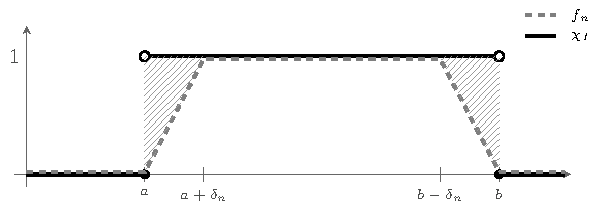
\includegraphics[scale=0.8]{figures/compact-supp-approx/main.pdf}
        \caption{Illustration of $f_n$ and $\chi_E$. Note that the hatched area represents $\lnorm \chi_I - f_n \rnorm_{L^1}$.}
        \label{fig:supp-int}
    \end{figure}

\section{Modes of Convergence}

\begin{definition}
    Let $(f_n)_n$ be a sequence of functions in $L^+$ and let $f \in L^+$.
    \begin{enumerate}[label = (\arabic*),itemsep=1pt,topsep=3pt]
        \item $f_n \rightarrow f$ \h2\textui{uniformly}\h2 if \h1 $\sup_{x \in X}|f(x) - f_n(x)| \rightarrow 0$.
        \item $f_n \rightarrow f$ \h2\textui{in $L^1$}\h2 if \h1 $\lnorm f - f_n(x)\rnorm_{L^1} \rightarrow 0$.
        \item $f_n \rightarrow f$ \h2\textui{in measure}\h2 if  for all $\epsilon > 0$, $\mu(\{x \mid |f_n(x) - f(x)| \geq \epsilon\}) \rightarrow 0$.
        \item $f_n$ is \textui{Cauchy in measure} if for all $\epsilon > 0$, $\mu(\{x \mid |f_n(x) - f_m(x)| \geq \epsilon\}) \rightarrow 0$.
    \end{enumerate}
\end{definition}

\begin{example}
    {\color{red} examples and pictures go here}
\end{example}

\begin{proposition}
    If $f_n \rightarrow f$ in $L^1$, then $f_n \rightarrow f$ in measure.
\end{proposition}
    \begin{proof}
        Let $\epsilon > 0$. For all $n \in \bfN$, define $E_n := \{x \mid |f_n(x) - f(x)| \geq \epsilon\}$. We have:
            \begin{equation*}
            \begin{split}
                \lnorm f - f_n \rnorm_{L^1} 
                & = \int |f - f_n| \\
                & \geq \int_{E_n} |f - f_n| \\
                & \geq \int_{E_n} \epsilon \\
                & = \epsilon \cdot \mu(E_n).
            \end{split}
            \end{equation*}
        Hence $\mu(E_n) \leq \frac{1}{\epsilon}\lnorm f - f_n \rnorm_{L^1}$. Since $\lnorm f - f_n \rnorm_{L^1} \rightarrow 0$ as $n \rightarrow \infty$, we have $\mu(E_n) \rightarrow 0$.
    \end{proof}

\begin{theorem}[Egorov's Theorem]
    Let $\mu(X) < \infty$. For each $n \in \bfN_0$, suppose $f_n$ is a measurable complex-valued function such that $f_n \rightarrow f_0$ pointwise almost everywhere. Then for all $\epsilon > 0$, there exists a measurable set $E \in \cM$ such that $\mu(E) < \epsilon$ and $f_n \rightarrow f$ uniformly on $E^c$.
\end{theorem}
    \begin{proof}
        Let $\epsilon > 0$. Define $A := \{x \mid f_n(x) \rightarrow f_0(x)\}$. By hypothesis $\mu(A^c) = 0$. For all $n,k \in \bfN$, define:
            \begin{equation*}
            \begin{split}
                E_n(k) = \bigcup_{m \geq n}\left\{x \in A \;\middle|\; |f_m(x) - f(x)| \geq \frac{1}{k}\right\}.
            \end{split}
            \end{equation*}
        For a fixed $k$, we have $E_{n}(k) \supset E_{n+1}(k)$ for all $n$, and $\bigcap_{n = 1}^\infty E_n(k) = \emptyset$. Since $\mu(X) < \infty$, we have $\mu(E_1) < \infty$, hence by continuity from above $\lim_{n \rightarrow \infty}\mu(E_n(k)) = 0$. Now for each $k$, choose $n_k$ such that:
            \begin{equation*}
            \begin{split}
                \mu(E_{n_k}(k)) < \frac{\epsilon}{2^k}.
            \end{split}
            \end{equation*}
        Define $E := A^c \cup \bigcup_{k = 1}^\infty E_{n_k}(k)$. We can see:
            \begin{equation*}
            \begin{split}
                \mu(E) 
                & = \mu\left(A^c \cup \bigcup_{k = 1}^\infty E_{n_k}(k)\right) \\
                & \leq \mu(A^c) + \mu \left( \bigcup_{k = 1}^\infty E_{n_k}(k) \right) \\
                & \leq 0 + \sum_{k = 1}^\infty \mu(E_{n_k}(k)) \\
                & < \sum_{k = 1}^\infty \frac{\epsilon}{2^k} \\
                & = \epsilon.
            \end{split}
            \end{equation*}
        Moreover, for all $x \in E^c$
    \end{proof}

\section{Integration in $\bfR^n$}

For the remainder of the section, fix $(X,\cM,\mu)$ and $(Y,\cN,\nu)$. We want to construct a measure on the measurable space $(X \times Y, \cM \otimes \cN)$.

\begin{definition}
    A \textui{rectangle} is a set $A \times B$, where $A \in \cM$ and $B \in \cN$.
\end{definition}

\begin{proposition}
    Let $\cA$ be the algebra containing all finite disjoint unions of rectangles. The function $\pi:\cA \rightarrow [0,\infty]$ given by $\pi(A \times B) := \mu(A)\nu(B)$ is a premeasure.
\end{proposition}
    \begin{proof}
        Let $A \times B$ be a rectangle that is a (finite or countable) disjoint union of rectangles $A_n \times B_n$. Note that:
            \begin{equation*}
            \begin{split}
                \chi_A(x)\chi_B(y)
                & = \chi_{A \times B}(x,y) \\
                & = \sum_{n}\chi_{A_n \times B_n}(x,y) \\
                & = \sum_{n}\chi_{A_n}(x)\chi_{B_n}(y). 
            \end{split}
            \end{equation*}
        Fix $y \in Y$ and integrate with respect to $x$. Then:
            \begin{equation*}
            \begin{split}
            \int_X \chi_A(x)\chi_B(y) d\mu(x) 
            & = \chi_B(y) \int_X \chi_A(x) d \mu(x) \\
            & = \int_X \sum_{n} \chi_{A_n}(x)\chi_{B_n}(y)d\mu(x) \\
            & = \sum_{n} \int_X \chi_{A_n}(x)\chi_{B_n}(y)d\mu(x) \\
            & = \sum_{n}\mu(A_n)\chi_{B_n}(y).
            \end{split}
            \end{equation*}
        Now integrate with respect to $y$. We similarly get:
            \begin{equation*}
            \begin{split}
                \int_Y \chi_A(x)\chi_B(y) d\nu(y) 
                & = \sum_{n} \chi_{A_n}
            \end{split}
            \end{equation*}
    \end{proof}












    \chapter{Differentiation}

\section{Signed Measures}
\begin{definition}
    Let $(X,\cM)$ be a measurable space. The map $\nu:\cM \rightarrow [-\infty,\infty]$ is a \textui{signed measure} if:
        \begin{enumerate}[label = (\arabic*),itemsep=1pt,topsep=3pt]
            \item $\nu(\emptyset) = 0$,
            \item $\{-\infty,\infty\} \not\subset \Image \nu$,
            \item If $\{E_i\}_{i = 1}^\infty \subset \cM$ is pairwise disjoint, and $\sum_{n = 1}^\infty \nu(E_n)$ is absolutely convergent whenever $\nu \left( \bigcup_{i = 1}^\infty E_i \right)$ is finite, then $\nu \left( \bigcup_{i = 1}^\infty E_i \right) = \sum_{i = 1}^\infty \nu(E_i)$
        \end{enumerate}
\end{definition}

Unless context is clear, we will refer to standard measures as \textit{positive measures}.

\begin{example}
\phantom{a}
\begin{enumerate}[label = (\arabic*),itemsep=1pt,topsep=3pt]
    \item If $\mu_1$ and $\mu_2$ are measures on $(X,\cM)$ and atleast one is finite, then $\nu:= \mu_1 - \mu_2$ is a signed measure.
    \item Let $f:X \rightarrow [-\infty,\infty]$ be measurable, $\mu$ a measure, and either $\int f^+ d\mu$ or $\int f^{-}d\mu$ be finite. Then $\nu(E) := \int_E f d\mu$ is a signed measure.
\end{enumerate}
\end{example}

\begin{definition}
    Let $\nu$ be a signed measure on $(X,\cM)$ and $E \in \cM$.
    \begin{enumerate}[label = (\arabic*),itemsep=1pt,topsep=3pt]
        \item $E$ is \textui{positive} if $\nu(F) \geq 0$ for all $F \in \cM$ with $F \subset E$.
        \item$E$ is \textui{negative} if $\nu(F) \leq 0$ for all $F \in \cM$ with $F \subset E$.
        \item $E$ is \textui{null} if $\nu(F) = 0$ for all $F \in \cM$ with $F \subset E$.
    \end{enumerate}
\end{definition}

\begin{proposition}\label{prop:properties-of-signed-measures}
    \phantom{a}
    \begin{enumerate}[label = (\arabic*),itemsep=1pt,topsep=3pt]
        \item If $\{E_n\}_{n=1}^\infty \subset \cM$ such that $E_1 \subset E_2 \subset E_3 \subset ...$, then $\nu \left( \bigcup_{n = 1}^\infty E_n \right) = \lim_{n \rightarrow \infty}\nu(E_n)$.
        \item If $\{E_n\}_{n=1}^\infty \subset \cM$ such that $E_1 \supset E_2 \supset E_3 \supset ...$, then $\nu \left( \bigcap_{n = 1}^\infty E_n \right) = \lim_{n \rightarrow \infty}\nu(E_n)$.
        \item Any measurable subset of a positive (resp. negative, null) set is positive (resp. negative, null).
        \item The countable union of positive (resp. negative, null) sets is positive (resp. negative, null).
        \item If $E \in \cM$ is positive (resp. negative, null) and $F \subset E$, then $\nu(F) \leq \nu(E)$ (resp. $\nu(F) \geq \nu(E)$, $\nu(F) = 0$).
    \end{enumerate}
\end{proposition}

\begin{theorem}[Hahn Decomposition Theorem]\label{thm:hdt}
    Let $\nu$ be a signed measure on $(X,\cM)$. There exists a positive set $P$ and a negative set $N$ such that:
    \begin{enumerate}[label = (\arabic*),itemsep=1pt,topsep=3pt]
        \item $P \cup N = X$;
        \item $P \cap N = \emptyset$;
        \item If $P'$ and $N'$ are another such pair satisfying (1) and (2), then $P \triangle P'$ and $N \triangle N'$ are null. 
    \end{enumerate}
\end{theorem}
    \begin{proof}
        Without loss of generality, suppose that $\nu$ does not take the value $+\infty$. Define:
            \begin{equation*}
            \begin{split}
                m:= \sup \{\nu(E) \mid E \in \cM, \text{ $E$ is positive}\}.
            \end{split}
            \end{equation*}
        Find a sequence of positive sets $\{E_n\}_{n = 1}^\infty$ such that $\nu(E_n) \rightarrow m$. Define $P := \bigcup_{n = 1}^\infty E_n$. Then $P$ is positive by (4) of Proposition~\ref{prop:properties-of-signed-measures}. Part (5) of Proposition~\ref{prop:properties-of-signed-measures} also gives $\nu(E_n) \leq \nu(P) \leq m$, hence by the squeeze theorem $\nu(P) = m$. Since $\nu$ does not take on the value $+\infty$, it must be the case that $m <+\infty$. Claim: The set $N:=X \setminus P$ is negative. 
        
        First, note that $N$ cannot contain a positive set of positive measure. Indeed, if $P' \subset N$ where $P'$ is positive and $\nu(P') > 0$, then $P \cup P'$ is positive and $\nu(P \cup P') = \nu(P) + \nu(P') > m$, which is a contradiction. 
        
        Second, if there exists a set $A \in \cM$ such that $A \subset N$ and $\nu(A) > 0$, then there exists another subset $B \subset N$ such that $\nu(B) > \nu(A)$. Indeed, we have just shown that $A$ cannot be positive, hence there exists a subset $C \subset A$ such that $\nu(C) < 0$. Therefore, $\nu(A \setminus C) = \nu(A) - \nu(C) > \nu(A)$.

        Now suppose towards contradiction $N$ is not negative. Then by definition there exists a set $A_1 \in \cM$ such that $A_1 \subset N$ and $\nu(A_1) > 0$. Find the smallest such $n_1 \in \bfN$ so that $\nu(A_1) > \frac{1}{n_1}$. By {\color{red}...DNF}

        Now suppose $P'$ and $N'$ are another such decomposition of $X$. Note that $P\setminus P' \subset P$, hence $\nu(P \setminus P') \geq 0$. But also $P \setminus P' = P \cap P^c = P \cap N \subset N$, hence $\nu(P \setminus P') \leq 0$. It must be the case that $\nu(P \setminus P') = 0$. This same argument gives $\nu(P' \setminus P) = \nu(N \setminus N') = \nu(N' \setminus N) = 0$. All together:
            \begin{equation*}
            \begin{split}
                0 & = \nu(P \setminus P') + \nu(P' \setminus P) = \nu(P \setminus P' \cup P' \setminus P) = \nu(P \triangle P'),\\
                0 & = \nu(N \setminus N') + \nu(N' \setminus N) = \nu(N \setminus N' \cup N' \setminus N) = \nu(N \triangle N').
            \end{split}
            \end{equation*}
        Thus the decomposition of $X$ is unique up to symmetric difference.
    \end{proof}

\begin{definition}
    Let $(X,\cM)$ be a measurable space. Two signed measures $\mu$ and $\nu$ are \textui{mutually singular} if there exists measurable sets $E,F \in \cM$ such that $E \cup F = X$, $E \cap F = \emptyset$, $E$ is null for $\mu$, and $F$ is null for $\nu$. We express this relationship symbolically as $\mu \bot \nu$.
\end{definition}

Informally, mutual singularity means that $\mu$ and $\nu$ "live on disjoint sets."

\begin{theorem}[Jordan Decomposition Theorem]\label{thm:jdt}
    If $\nu$ is a signed measure on $(X,\cM)$, there exist unique positive measures $\nu^+,\nu^-$ such that $\nu = \nu^+ - \nu^-$ and $\nu^+ \bot \nu^-$.
\end{theorem}
    \begin{proof}
        By the Hahn Decomposition Theorem, we can write $X = P \cup N$, where $P$ is positive, $N$ is negative, and $P \cap N = \emptyset$. Define $\nu^+(E) = \nu(E \cap P)$ and $\nu^-(E) = -\nu(E \cap N)$. Then $\nu^+$ and $\nu^-$ are positive measures and clearly $\nu^+ \bot \nu^-$.

        Suppose $\nu = \mu^+ - \mu^-$ is another such decomposition such that $\mu^+$ and $\mu^-$ are positive and $\mu^+ \bot \mu^-$. Let $E,F \in \cM$ such that $E \cup F = X$, $E \cap F = \emptyset$, and $E$ is $\mu^-$-null and $F$ is $\mu^+$-null. Let $E'$ be any subset of $E$. Then $\nu(E') = \mu^+(E') - \mu^-(E') \geq \mu^+(E') \geq 0$. Hence $E$ is positive. A similar argument can be used to show that $F$ is negative. Thus $E \cup F$ is another Hahn decomposition of $X$. This means $P \triangle E$ is $\nu$-null and $N \triangle F$ is $\nu$-null. For any $A \in \cM$ we have:
            \begin{equation*}
            \begin{split}
                \mu^+(A)
                & = \mu^+(A \cap E) + \mu^+(A \cap P) \\
                & = 
            \end{split}
            \end{equation*}
        {\color{red} ... DNF}
    \end{proof}

\begin{definition}
Let $(X,\cM)$ be a measurable space and $\nu$ a signed measure.
\begin{enumerate}[label = (\arabic*),itemsep=1pt,topsep=3pt]
    \item The \textui{total variation} of $\nu$ is $|\nu| := \nu^+ + \nu^-$.
    \item $\nu$ is \textui{finite} (resp. $\sigma$-finite) if $|\nu|$ is finite (resp. $\sigma$-finite).
    \item Let $\mu$ be a positive measure. We say $\nu$ is \textui{absolutely continuous with respect to $\mu$}, and write $\nu \ll \mu$, if for all $E \in \cM$, $\mu(E) = 0$ implies $\nu(E) = 0$.
\end{enumerate}
\end{definition}

\begin{example}
    {\color{red} some examples go here...}
\end{example}

\begin{lemma}
    Let $(X,\cM)$ be a measurable space. Let $\nu$ be a signed measure and $\mu$ a positive measure. The following are equivalent:
    \begin{enumerate}[label = (\arabic*),itemsep=1pt,topsep=3pt]
        \item $\nu \ll \mu$;
        \item $\nu^+ \ll \mu$ and $\nu^- \ll \mu$.
        \item $|\nu| \ll \mu$;
    \end{enumerate}
\end{lemma}
    \begin{proof}
        ({\small 1$\Rightarrow$2}) Let $E \in \cM$. Suppose $\mu(E) = 0$. Then $\nu(E) = 0$. By the \nameref{thm:hdt}, there exists $P,N \in \cM$ such that $P \cup N = X$, $P \cap N = \emptyset$, $P$ is positive, and $N$ is negative. By the monotonicity of $\mu$, we have $\mu(E \cap P) \leq \mu(E) = 0$, hence $\mu(E \cap P) = 0$. Similarly, $\mu(E \cap N) \leq \mu(E) = 0$, hence $\mu(E \cap N) = 0$. The \nameref{thm:jdt} says $\nu$ can be written as $\nu^+ - \nu^-$, where $\nu^+(E) = \nu(E \cap P)$ and $\nu^-(E) = \nu(E \cap N)$. Since $\mu(E \cap P) = 0$, we have $\nu(E \cap P) = \nu^+(E) = 0$. Since $\mu(E \cap N) = 0$, we have $\nu(E \cap N) = \nu^-(E) = 0$.

        ({\small 2$\Rightarrow$3}) If $E \in \cM$ such that $\mu(E) = 0$, then $|\nu|(E) = \nu^+(E) + \nu^-(E) = 0$.

        ({\small 3$\Rightarrow$1}) If $E \in \cM$ such that $\mu(E) = 0$, then $|\nu|(E) = \nu^+(E) + \nu^-(E) = 0$. Since $\nu^+$ and $\nu^-$ are positive measures by the \nameref{thm:jdt}, it must be the case that $\nu^+(E) = 0$ and $\nu^-(E) = 0$. Hence $\nu^+(E) - \nu^-(E) = \nu(E) = 0$. 
    \end{proof}

\begin{proposition}
Let $(X,\cM)$ be a measurable space. Let $\nu$ be a finite signed measure and $\mu$ a positive measure. Then $\nu \ll \mu$ if and only if for all $\epsilon > 0$, there exists $\delta > 0$ such that for all $E \in \cM$, $\mu(E) < \delta$ implies $|\nu|(E) < \epsilon$.
\end{proposition}
    \begin{proof}
        ($\Leftarrow$) Let $\mu(E) = 0$. Let $\epsilon = \frac{1}{n}$. By hypothesis, there exists $\delta > 0$ such that $\mu(E) < \delta$ implies $|\nu|(E) < \frac{1}{n}$. Since $\nu(E) = 0 < \delta$, surely $|\nu|(E) < \frac{1}{n}$. Taking $n \rightarrow \infty$ gives $|\nu|(E) = 0$. Hence $|\nu| \ll \mu$, which is equivalent to $\nu \ll \mu$.

        ($\Rightarrow$) We prove the contrapositive for this direction. Suppose the $\epsilon$-$\delta$ condition is not satisfied. Then there exists $\epsilon > 0$ such that for all $n \in \bfN$, there exists $E_n \in \cM$ such that $\mu(E_n) < \frac{1}{2^n}$ and $|\nu|(E) \geq \epsilon$. Define $F_k := \bigcup_{n = k}^\infty E_n$ and $F := \bigcap_{k = 1}^\infty F_k$. Then $\mu(F_k) < \sum_{n = k}^\infty \frac{1}{2^n} = \frac{1}{2^{k-1}}$, hence $\mu(F) = 0$. Since $\nu$ is finite, by continuity from below $|\nu|(F) = \lim_{n \rightarrow \infty}|\nu|(F_k) \geq \epsilon$. Thus it is false that $\nu \ll \mu$.
    \end{proof}

\begin{theorem}[Lebesgue-Radon-Nikodym Theorem]\label{thm:lrnt}
Let $(X,\cM)$ be a measurable space. Let $\mu$ be a $\sigma$-finite positive measure and $\nu$ a $\sigma$-finite signed measure. Then there exist unique $\sigma$-finite signed measures $\nu_s$ and $\nu_{ac}$ such that:
    \begin{enumerate}[label = (\arabic*),itemsep=1pt,topsep=3pt]
        \item $\nu = \nu_\text{s} + \nu_\text{ac}$;
        \item $\nu_\text{s} \bot \mu$;
        \item $\nu_\text{ac} \ll \mu$.
    \end{enumerate}
Moreover, there exists an extended $\mu$-integrable function $f:X \rightarrow \bfR$ (i.e., either $\int f^+ d\mu < \infty$ or $\int f^- d\mu < \infty$) such that:
\begin{enumerate}[label = (\arabic*),itemsep=1pt,topsep=3pt]
    \addtocounter{enumi}{3}
    \item $d\nu_\text{ac} = f d\mu$,
\end{enumerate}
and if $g$ is another such function satisfying (4), then $f = g$ a.e.
\end{theorem}
    \begin{proof}
        We first assume that $\nu$ and $\mu$ are both positive, finite, and $\nu \ll \mu$. Claim: there exists $f:X \rightarrow [0,\infty)$, $f \geq 0$ such that $d \nu =f d\mu$. Define:
            \begin{equation*}
            \begin{split}
                \cF := \{f:X \rightarrow [0,\infty) \text{ measurable} \mid \text{ for all }E \in \cM, {\ts \int_E} f d\mu \leq \nu(E)\}.
            \end{split}
            \end{equation*}
        {\color{red} oop}
    \end{proof}

\begin{definition}
    Using the terminology of Theorem~\ref{thm:lrnt}:
    \begin{enumerate}[label = (\arabic*),itemsep=1pt,topsep=3pt]
        \item the decomposition $\nu = \nu_{\text{s}} + \nu_{\text{ac}}$ is called a \textui{Lebesgue decomposition};
        \item In the case that $\nu = \nu_{\text{ac}}$, we say $f$ is the \textui{Radon-Nikodym derivative of $\nu$ with respect to $\mu$}, and write $f = \frac{d\nu}{d\mu}$.
    \end{enumerate}
\end{definition}

\iffalse
\begin{figure}[h]
\centering
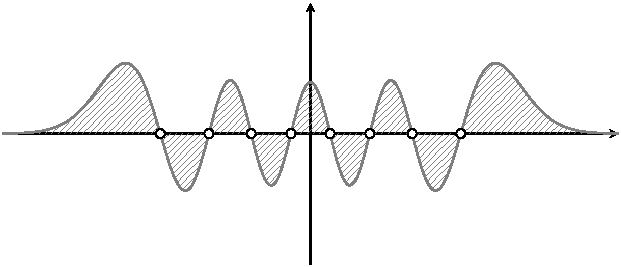
\includegraphics[scale=0.8]{figures/hahn-decomp-theorem/main}
\caption{On $(\bfR,\mathcal{L})$ let $m$ be Lebesgue measure and define the signed measure $\nu(E)=\int_E f\,dm$. The shading indicates the positive ($f\ge 0$) and negative ($f\le 0$) contributions of $f$. By part (3) of the Hahn Decomposition Theorem, the decomposition $\bfR=P\cup N$ is unique up to null sets. Indeed, taking $P=\{x \mid f(x) \geq 0\}$, $P' = \{x \mid f(x) > 0\}$, $N = \{x \mid f(x) < 0\}$, and $N' = \{x \mid f(x) \leq 0\}$, we have that the sets $P \triangle P'$ and $N \triangle N'$ are null.}
\label{fig:hahn-decomp-theorem}
\end{figure}
\fi













\end{document}
